\chapter{Jugando contra adversarios justos en juegos estocásticos}
\label{cap:fairAdversaries}


\section{Introduction} \label{sec:intro}
	Game theory \cite{MorgensternNeuman42}  admits an elegant and profound mathematical theory. 
	In the last decades, it has received widespread attention from computer scientists because it has important applications to software synthesis and verification. 
	The analogy is appealing, the operation of a system under an uncooperative environment (faulty hardware, malicious agents, unreliable communication channels, etc.) can be modeled as a game 
	between two players (the system and the environment), in which the system tries to fulfill certain goals, whereas the environment tries to prevent this from happening. 
	This view is particularly useful for \emph{controller synthesis}, i.e., to automatically generate decision-making policies from high-level specifications. 
	Thus, synthesizing a controller consists of computing optimal strategies for a given game.
		
	In this paper we  focus on zero-sum, perfect-information, two-player, turn-based stochastic games with (non-negative) rewards \cite{FilarV96}. 
	Intuitively, these games are played in a graph by two players who move a token in turns. Some vertices are probabilistic, in the sense that, if a token is in a probabilistic vertex, then 
	the next vertex is randomly selected. Furthermore, the players select their moves using strategies. Associated with each vertex there is a reward (which, in this paper, is taken to be non-negative).
	The goal of Player $1$ is to maximize the expected amount of collected rewards during the game, whereas Player $2$ aims at minimizing this value. 
	This is what~\cite{SvorenovaKwiatkowska16} calls \emph{total reward objective}.
	These kinds of games have been shown useful to reason about several classes of systems such as autonomous vehicles, 
	fault-tolerant systems, communication protocols, energy production plants, etc.  %(See~\cite{SvorenovaKwiatkowska16} for concrete case studies.)
        Particularly, in this paper we consider those games in which one of the players employs fair strategies. 

	Fairness restrictions, understood as fair resolutions of non-determinism of actions, play an important role in software verification and controller synthesis. 
	Especially, fairness assumptions over environments make possible the verification of liveness properties on open systems. 
	Several authors have indicated the need for fairness assumptions over the environment 
	in the controller synthesis approach, e.g., \cite{DBLP:conf/fossacs/AsarinCV10,DBLP:conf/icse/DIppolitoBPU11}.
        As a simple example consider an autonomous vehicle that needs to traverse a field where moving objects may interfere in its path.  Though the precise behavior of the objects may be unknown, it is reasonable to assume that they will not continuously obstruct the vehicle attempts to avoid them.  In this sense, while stochastic behavior may be a consequence of the vehicle faults, we can only assume a fair behavior of the surrounding moving objects.
        %% As a simple example consider a communication protocol that transmits bits between two or  more processes via an unreliable channel. 
	%% Clearly, no protocol can guarantee the transmission of information if the environment (i.e., the channel) always loses messages.  Similarly, and to provide more examples, we can assume that a processing module will never receive an infinite number of jobs within a time unit, or that a repairable piece of hardware will not be breaking continuously preventing the development of a particular task, etc.
        In this work, we consider stochastic games in which one of the players (the one playing the environment) is assumed to play only with strong fair strategies.
%% \remarkPC{Los ejemplos que damos aca podrian solucionarse si las fallas tienen probabilidades, habría que buscar un ejemplo que muestre la necesidad de fairness aun con randomized environments.}	
%        In all of these cases, it is sensible to assume that the environments show a \emph{strong fair} behaviour.
 %       In this work, we consider stochastic games in which one of the players (the one playing the environment) is assumed to play only with strong fair strategies.
%	\textcolor{red}{This is true even for randomized controllers. For example, consider a randomized arbiter (as the one described in \cite{DBLP:conf/ifm/Baier10}), the arbiter 
%	grants the access to a mutually exclusive resource to two processes running in an asynchronous manner. When both processes want to access to the resource,  the arbiter tosses an unbiased coin to select one of the competing processes. 
%	The protocol cannot guarantee that both  processes will eventually have access to the resource, unless  fairness assumptions are made over the scheduling policy.
%	In these kinds of scenarios it is sensible to assume that the environments show a \emph{strong fair} behaviour.
%        In this work, we consider stochastic games in which one of the players (the one playing the environment) is assumed to play only with strong fair strategies.
%	}
%	As a simple example consider a communication protocol that transmits bits between two or  more processes via an unreliable channel. 
%	Clearly, no protocol can guarantee the transmission of information if the environment (i.e., the channel) always loses messages.  
%        In this sense, it is reasonable to expect that not every message that is sent will be eventually lost.
%        Similarly, and to provide more examples, we can assume that a processing module will never receive an infinite number of jobs within a time unit, or that a repairable piece of hardware will not be breaking continuously preventing the development of a particular task, etc.
%        In all of these cases, it is sensible to assume that the environments show a \emph{strong fair} behaviour.
 %       In this work, we consider stochastic games in which one of the players (the one playing the environment) is assumed to play only with strong fair strategies.

        In order to guarantee that the expected value of accumulated rewards is well defined in (perhaps infinite) plays, some kind of stopping criteria is needed.  A common way to do this is to force the strategies to decide to stop with some positive probability in every decision.  This corresponds to the so-called discounted stochastic games~\cite{Shapley1095,FilarV96}, and has the implications that the collected rewards become less important  as the game progresses (the ``importance reduction'' is given by the discount factor).  Alternatively, one may be interested in knowing the expected \emph{total} reward, that is, the expected accumulated reward \emph{without} any loss of it as time progresses.  For this value to be well defined, the game itself needs to be stopping. That is, no matter the strategies played by the players, the probability of reaching a terminal state needs to be $1$~\cite{Condon90,FilarV96}.
	%% In this work we consider stochastic games in which we have fairness assumptions over one of the players (the environment). Usually, some stopping criteria is used for 
	%% guaranteeing that the expected value of total reward is well-defined in (perhaps infinite) plays. This can be done in different ways, either using discounted rewards functions \cite{Shapley1095,FilarV96} or 
	%% assuming that a \emph{terminal} state will be reached with probability $1$ \cite{Condon90,FilarV96}.
        We focus on this last type of game.  However, we study here games that may not be stopping in general (i.e., for every strategy), but instead, require that they become stopping only when the minimizer plays in a fair way.  
	%% We study here games that may be not stopping in general, but they become stopping when the minimizer plays in a fair way.
        We use a  notion of (almost-sure) strong fairness, mostly following the ideas introduced in~\cite{DBLP:journals/dc/BaierK98} for Markov decision processes. We show that these kinds of games are determined, i.e., each state of the game has a value defined.  Furthermore, we show that memoryless and deterministic optimal  strategies exist for both players. Moreover, the value of the game can be calculated via the greatest fixed point of the corresponding functionals. 
It is important to remark that most of the properties discussed in this paper hold when the fairness assumptions are  made over the minimizer. Similar properties may not hold if the role of players is changed. 
However, these conditions encompass a large class of scenarios, where the system intends to maximize the total collected reward and the environment has the opposite objective.

%\paragraph{Contributions.} 
In summary,  the contributions of this paper are the following: (1) we introduce  the notion of stopping under fairness stochastic game, a generalization of stopping game that takes into account fair environments; (2) we prove that it can be decided in polynomial time whether a game is stopping under fairness; (3) we show that  these kinds of games are determined and both players possess optimal stationary strategies,  which can be computed using Bellman equations; and (4) we implemented these ideas in a prototype tool embedded in the {\PrismGames} toolset~\cite{DBLP:conf/cav/KwiatkowskaN0S20}, which we used to evaluate the viability of our approach through practical case studies.
%\paragraph{Structure.}


%%%%%%%%%%%%%%%%%%%%%%%%%%%%%%%%%%%%%%%%%%%%%%%%%%%%%%%%%%%%%%%%%%%%%%%%%
%% PARA LA POSIBLE VERSION FINAL:
%% Considerar revertir este p\'arrafo al que est\'a comentado debajo
%% dado que lo mutil\'e un poco para reducir espacio.
%%%%%%%%%%%%%%%%%%%%%%%%%%%%%%%%%%%%%%%%%%%%%%%%%%%%%%%%%%%%%%%%%%%%%%%%%
The paper is structured as follows. Section \ref{sec:mot_example} introduces an illustrating example to motivate the use of having fairness restrictions over the minimizer.  Section \ref{sec:background} fixes terminology and introduces background concepts. 
In Section \ref{sec:fair-strats} we describe a polynomial procedure to check whether a game stops under fairness assumptions, 
we also prove that determinacy is preserved in these games as well as the existence of (memoryless and deterministic) optimal strategies. 
Experimental results are described in Section \ref{sec:experimental_eval}. 
Finally, Sections \ref{sec:related_work} and  \ref{sec:conclusions} discuss related work and draw some conclusions, respectively.  Full proofs are gathered in the Appendix.

%% The paper is structured as follows. Section \ref{sec:mot_example} introduces an illustrating example to motivate the usefulness of having fairness restrictions over the minimizer on stochastic games. Section \ref{sec:background} fixes terminology and introduces background concepts. 
%% In Section \ref{sec:fair-strats} we describe a polynomial procedure to check whether a game stops under fairness assumptions, 
%% we also prove that determinacy is preserved in these games as well as the existence of (memoryless and deterministic) optimal strategies. 
%% Experimental results are described in Section \ref{sec:experimental_eval}. 
%% Finally, in Sections \ref{sec:related_work} and  \ref{sec:conclusions} we discuss related work and draw some conclusions, respectively.  Due to space constraints,  full proofs are gathered in the Appendix.



\newcommand{\roborta}{Roborta\xspace}

\section{\roborta vs.\ the Fair Light (A Motivating Example)} \label{sec:mot_example}

\begin{wrapfigure}[18]{l}{78mm}
\vspace{-11.6mm}
{\fontsize{6.6}{6.6}\selectfont\ttfamily
\begin{tabbing}
x\=xxxxxxxxxx\=xxxxxx\=xxx\=xxxx\=xxx\=xxxx\= \kill    
module \roborta\_vs\_the\_light\\[1ex]
\>col : [0..WIDTH] init 0; \\
\>row : [0..LENGTH] init 0; \\
\>light : [0..3] init 0; \>\>\>\> // current light color \\%[1ex]
\>                   \>\>\>\>// 0: red (light's turn) \\%[1ex]
\>                   \>\>\>\>// 1: yellow (\roborta moves sideways) \\%[1ex]
\>                   \>\>\>\>// 2: green (\roborta moves foreward) \\%[1ex]
\>                   \>\>\>\>// 3: off (light fails, any move) \\[1ex]
%\> // board allowed movements: 0:left, 1:both, 2:right \\[1ex]
\> // light moves \\[1ex]
\>[l\_y] (light=0) \> \>-> \>(1-Q) : (light'=1) + Q : (light'=3);\\[1ex]
\>[l\_g] (light=0) \> \>-> \>(1-Q) : (light'=2) + Q : (light'=3);\\[1ex]
%% \>[l\_y] (light=0) \> \>-> \>(1-Q) : (light'=1) + \\
%% \> 					 \> \> \> Q : (light'=3);\\[1ex]
%% \>[l\_g] (light=0) \> \>-> \>(1-Q) : (light'=2) + \\
%% \> 					 \> \> \> Q : (light'=3);\\[1ex]
\> // \roborta moves \\[1ex]
\>[r\_l]  ((light=1) | (light=3)) \& (MOVES[col,row] <= 1)  \\
\>                    \>\>-> \>(1-P) : (light'=0) \& (col'=(col-1)\%WIDTH) + \\       
\>                     \>\>\>  P : (light'=0) ; \\[1ex]

\>[r\_r] ((light=1) | (light=3)) \& (MOVES[col,row] >= 1)\\
\>                    \>\>-> \> (1-P) : (light'=0) \& (col'=(col+1)\%WIDTH) + \\
\>                     \>\>\> P : (light'= 0); \\[1ex]
\>[r\_f] ((light=2) | (light=3)) \& (row < LENGTH) \\
\>                    \>\>-> \> (1-P) : (light'=0) \& (row'=row+1)  + \\
\>                     \>\>\> P : (light'= 0);\\[1ex]
endmodule\\[-5ex]
\end{tabbing}}
\caption{Model for the  Game} \label{fig:robot_game_model}
\end{wrapfigure}
		Consider the following scenario. \roborta the robot is navigating a grid of $4 \times 4$ cells. There is a light signal  
determining the possible movements of the robot: if the light is yellow, she must move  sideways (at a border cell, \roborta is allowed to wrap around to the other side); if the light is green she ought to move forward; if the light is red, she cannot perform any movement; if the light is off, the robot is free to move either sideways or forward.  The light signal and \roborta change their states in turns.  A (non-negative) reward is associated with each location of the grid.  Also, the sideway movements can be restricted to only one direction in some locations.
Moreover, we consider possible failures on the behavior of the robot and the light. If \roborta fails, she loses her turn to move, and if the light fails, it turns itself off.  The failures occur with a given probability. The goal of \roborta is to collect as many rewards as possible.  In opposition, the light aims at minimizing this value.
The specification of this game is captured in Fig.~\ref{fig:robot_game_model} (using {\Prism}-like notation \cite{DBLP:conf/cav/KwiatkowskaNP11}). 
%% %
%% \begin{wrapfigure}[11]{r}{52mm}
%% \vspace{-5mm}
%% {\fontsize{6.6}{6.6}\selectfont\ttfamily
%% \centering
%% 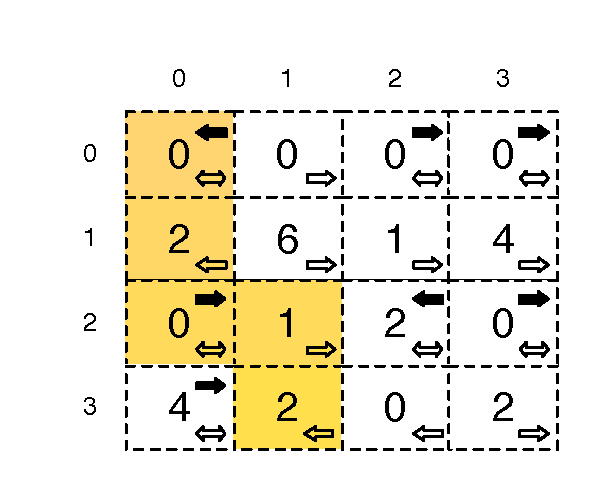
\includegraphics[scale=0.45]{Figs/robotMovesRewards.eps}\hspace{1em}\mbox{}}
%% \caption{A robot on a $4 \times 4$ grid} \label{fig:robot_game_grid}
%% \end{wrapfigure}
%% 
%% \noindent
In this model, \texttt{WIDTH} and \texttt{LENGTH} are constants defining the dimension of the grid.  \texttt{MOVES} is a two-dimensional array modeling the possible sideways movements in the grid (\texttt{0} allows the robot to move only to the left, \texttt{1}, to either side, and \texttt{2}, only to the right).  \texttt{P} and \texttt{Q}  define the failure probabilities of \roborta and the light respectively.
%The rewards assigned to each location of the grid are stored in a matrix named \texttt{REWARDS}.
Fig.~\ref{fig:robot_game_grid} shows the assignment of rewards to each location of the $4 \times 4$ grid as well as the sideway movement restrictions (shown on the bottom-right of each location with white arrows).
The game starts at the location $(0, 0)$ and it stops when \roborta escapes through the end of the grid.


\begin{wrapfigure}[11]{r}{48mm}
\vspace{-9mm}
{\fontsize{6.6}{6.6}\selectfont\ttfamily
\centering
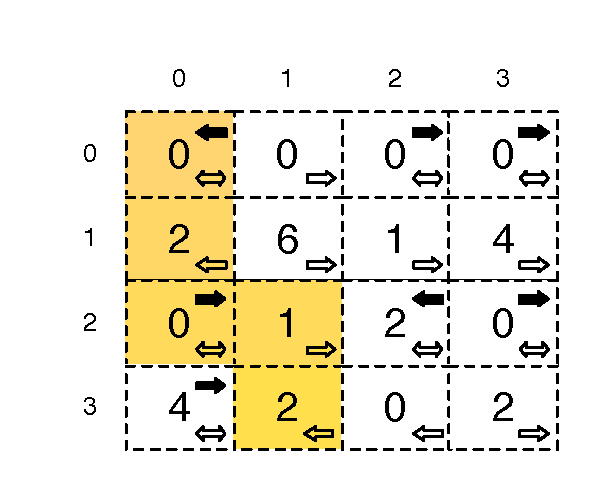
\includegraphics[scale=0.45]{Figs/robotMovesRewards.eps}\hspace{1em}\mbox{}}
\caption{A robot on a $4 \times 4$ grid} \label{fig:robot_game_grid}
\end{wrapfigure}
	%A possible scenario in this game is as follows. The robot is in cell $(0,2)$ and the light is yellow, thus the robot can only move to locations $(0, 1)$ or $(0, 3)$. 
	A possible scenario in this game is as follows. \roborta starts in cell $(0,0)$ and, in an attempt to minimize the rewards accumulated by the robot, the environment switches the yellow light on.
	For the sake of simplicity, we assume no failures on the light, i.e., $\texttt{Q}=0$. 
	Notice that, if the environment plays always in this way (signaling a yellow light), then \roborta will never achieve the goal and 
the game never stops.  This scenario occurs when the light plays in an unfair way, i.e., an action (the one that turns the green light on) is enabled infinitely often, but it is not executed infinitely often.
	Assuming fairness over the environment, we can ensure that a green light will be eventually switched on, allowing the robot to move forward.

	The best strategy for \roborta when the light is yellow is shown in black arrows on the top-right of the locations without movement restrictions.
	%As a result, the best strategy to achieve the goal for the robot can be observed in the highlighted portion of the grid in yellow in
	As a result, when both players play their optimal strategies, the path taken by \roborta to achieve the goal can be observed in the yellow-highlighted portion of the grid  in
Fig.~\ref{fig:robot_game_grid}.  In Section \ref{sec:experimental_eval}, we evaluate this problem experimentally with different 
configurations of this game.

\iffalse
\begin{figure}[t]
\begin{minipage}[b]{0.45\linewidth}
\fontsize{6.6}{6.6}\selectfont\ttfamily
\begin{tabbing}
x\=xxxxxxxxxx\=xxxxxx\=xxx\=xxxx\=xxx\=xxxx\= \kill    
module RobotGame\\[1ex]
\>col : [0..WIDTH] init 0; \\
\>row : [0..LENGTH] init 0; \\
\>light : [0..3] init 0; \>\>\>\> // current light color \\%[1ex]
\>                   \>\>\>\>// 0: red (light's turn) \\%[1ex]
\>                   \>\>\>\>// 1: yellow (robot moves sideways) \\%[1ex]
\>                   \>\>\>\>// 2: green (robot moves forward) \\%[1ex]
\>                   \>\>\>\>// 3: off (light fails, any move) \\[1ex]
%\> // board allowed movements: 0:left, 1:both, 2:right \\[1ex]
\> // light moves \\[1ex]
\>[l\_y] (light=0) \> \>-> \>(1-Q) : (light'=1);\\
\> 					 \> \>-> \> Q : (light'=3);\\[1ex]
\>[l\_g] (light=0) \> \>-> \>(1-Q) : (light'=2);\\
\> 					 \> \>-> \> Q : (light'=3);\\[1ex]
\> // robot moves \\[1ex]
\>[r\_l]  ((light=1) | (light=3)) \& (MOVES[col,row] <= 1)  \\
\>                    \>\>-> \>(1-P): (light'=0) \& (col'=(col-1)\%WIDTH) + \\       
\>                     \>\>\>  P: (light'=0) ; \\[1ex]

\>[r\_r] ((light=1) | (light=3)) \& (MOVES[col,row] >= 1)\\
\>                    \>\>-> \> (1-P : (light'=0) \& (col'=(col+1)\%WIDTH) + \\
\>                     \>\>\> P: (light'= 0); \\[1ex]
\>[r\_f] ((light=2) | (light=3)) \& (row < LENGTH) \\
\>                    \>\>-> \> (1-P): (light'=0) \& (row'=row+1)  + \\
\>                     \>\>\> P: (light'= 0);\\[1ex]
endmodule\\[-5ex]
\end{tabbing}
\caption{Model for the Robot Game} \label{fig:robot_game_model}
\end{minipage}
\hspace{0.5cm}
\begin{minipage}[b]{0.45\linewidth}
\fontsize{6.6}{6.6}\selectfont\ttfamily
\centering
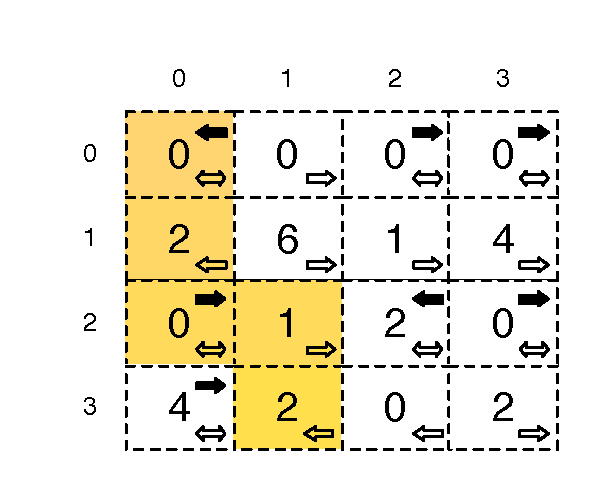
\includegraphics[scale=0.45]{Figs/robotMovesRewards.eps}\hspace{4em}\mbox{}

\vspace{7em}
\caption{A robot on a $4 \times 4$ grid} \label{fig:robot_game_grid}
\end{minipage}
\end{figure}
\fi


\section{Stopping Games and Fair Strategies}\label{sec:fair-strats}

We begin this section by introducing the notions of \emph{(almost sure) fair strategy} and \emph{stopping games under fairness}. 
%%
%% It is worth noting that most of the definitions below  can be applied to both players. However, from now on, we assume that Player $2$ represents the environment,  which tries to minimize the amount of rewards obtained by the system, thus  fairness restrictions will be applied to this player. 
%%
From now on, we assume that Player $2$ represents the environment,  which tries to minimize the amount of rewards obtained by the system, thus  fairness restrictions will be applied to this player. 

%intuitively, one player represents the environment and the other represents the system. In our setting, the environment  wants to minimize the amount of rewards obtained by the system (clock ticks, bits successfully transmitted, etc), and the system wants to maximize these rewards. 
%In the following, we assume that Player $2$ is the environment, thus from now on fairness restrictions are applied to this player. 
\begin{definition}
   Given a stochastic game $\StochG = (V, (V_1, V_2, V_\Probabilistic), \delta)$.
The set of fair plays for Player $2$ (denoted $\FP^2$) is defined as follows:
\[
	\FP^2 = \{ \omega \in \GamePaths_{\StochG} \mid \forall v' \in V_2: v' \in \inf(\omega)  \Rightarrow \post(v') \subseteq \inf(\omega) \}
\]
%%    Given a stochastic game $\StochG = (V, (V_1, V_2, V_\Probabilistic), \delta)$ and  $i \in \{1,2\}$.
%% The set of fair plays for Player $i$ from vertex $v$ (denoted $\FP^i_v$) is defined as follows:
%% \[
%% 	\FP^i_v = \{ \omega \in \GamePaths_{\StochG,v} \mid \forall v' \in V_i: v' \in \inf(\omega)  \Rightarrow \post(v') \subseteq \inf(\omega) \}
%% \]
\end{definition}
	Alternatively,  if we consider each vertex as a proposition,  $\FP^2$ can be written using {\LTL} notation as: 
	$\bigwedge_{v \in V_2} \bigwedge_{v' \in \post(v)}(\Box \Diamond v \Rightarrow \Box \Diamond v')$.  This property is 	 $\omega$-regular, thus it is measurable  in the $\sigma$-algebra generated by the cones of $\GamePaths_{\StochG}$ (see e.g., \cite[p.804]{BaierK08}). This is a state-based notion of fairness, but it can be straightforwardly extended to settings where transitions are considered. For the sake of simplicity we do not do so in this paper.
	
%	Note that the set of fair plays is $\omega$-regular, thus it is measurable  in the $\sigma$-algebra generated by the cones of $\GamePaths_{\StochG}$ \cite{Katoen08}. 
	
	%% The following definition introduces the notion of  (almost-sure) \emph{fair strategies} for Player $2$.
	Next, we introduce the notion of  (almost-sure) \emph{fair strategies} for Player $2$.
        %% (Almost-sure) fair strategies for Player $1$ are defined analogously. 
\begin{definition} Given a stochastic game $\StochG = (V, (V_1, V_2, V_\Probabilistic), \delta)$,
a strategy $\strat{2} \in \Strategies{2}$ is said to be \emph{almost-sure fair} (or simply \emph{fair}) iff it holds that:
%$\Prob{\strat{1}}{\strat{2}}_{\StochG,v}(\FP^2_v) = 1$,
$\Prob{\strat{1}}{\strat{2}}_{\StochG,v}(\FP^2) = 1$,
for every $\strat{1} \in \Strategies{1}$ and $v \in V$. 
\end{definition}
%
The set of all the  fair strategies for Player $2$ is denoted by $\FairStrats{2}$. We combine this notation  with the notation introduced in Section \ref{sec:background}, e.g., $\MemorylessFairStrats{2}$ refers to the set of all  memoryless and fair strategies for Player $2$. 
%
The previous definition is based on the notion of fair scheduler as introduced for Markov decision processes~\cite{DBLP:journals/dc/BaierK98,BaierK08}.

Note that for stopping games, every strategy is fair, because the probability of visiting a vertex infinitely often is $0$.
%
Also notice that there are games which are not stopping, but they become stopping if Player $2$ uses only fair strategies. This is the main idea behind the notion of \emph{stopping under fairness} as introduced in the following definition.
	
\begin{definition}\label{def:stopping-under-fairness}
  A stochastic game $\StochG = (V, (V_1, V_2, V_\Probabilistic), \delta)$ is said  to be \emph{stopping under fairness} iff for all strategies $\strat{1} \in \Strategies{1}, \strat{2} \in \FairStrats{2}$ and vertex $v \in V$, it holds that
  $\Prob{\strat{1}}{\strat{2}}_{\StochG,v}(\Diamond T)=1$,  where $T$ is the set of terminal vertices of $\StochG$. 
\end{definition}

%\remarkPRD{Considerar agregar un ejemplo con \textbf{Roborta}}

%\subsection{Checking the stopping criteria}
\paragraph{Checking stopping criteria.}

This section is devoted to the effective
characterization of games that are stopping under fairness.
%% The next part of this section is devoted to the effective
%% characterization of games that are stopping under fairness.
The
following lemma states that, for every game that is not stopping under
fairness, there is a \emph{memoryless deterministic} strategy for
Player 1 and a fair strategy for Player 2 that witnesses it.


\begin{lemma}\label{lemma:memoryless-strat}
  Let $\StochG = (V, (V_1, V_2, V_\Probabilistic), \delta)$ be a
  stochastic game, $v \in V$, and $T$ the set of terminal states of $\StochG$.
  %
  If $\Prob{\strat{1}}{\strat{2}}_{\mathcal{G}, v}(\Diamond T) < 1$
  for some
  $\strat{1} \in \Strategies{1}$ and $\strat{2} \in \FairStrats{2}$,
  then, for some memoryless and deterministic strategy
  $\strat{1}' \in \DetMemorylessStrats{1}$ and fair strategy
  $\strat{2}' \in \FairStrats{2}$,
  $\Prob{\strat{1}'}{\strat{2}'}_{\mathcal{G}, v}(\Diamond T) < 1$.
\end{lemma}


The proof of this lemma follows by noticing that, if
$\Prob{\strat{1}}{\strat{2}}_{\mathcal{G}, v}(\Diamond T) < 1$, there
must be a finite path that leads with some probability to an end
component not containing a terminal state and which is a trap for the
fair strategy $\strat{2}$.  This part of the game enables the
construction of a memoryless deterministic strategy for Player 1 by
ensuring that it follows the same finite path (but skipping loops) and
that it traps Player 2 in the same end component.

	
The next theorem states that checking stopping under fairness in a
stochastic game $\StochG$ can be reduced to check the stopping
criteria in a MDP, which is obtained from $\StochG$ by fixing a strategy in
Player 2 that selects among the output transitions according to a
uniform distribution.  Thus, this theorem enables a graph solution to
determine stopping under fairness.

%The next theorem is central to reduce the problem of checking whether a game is stopping to that of checking whether an MDP version of it is stopping.

\begin{theorem}\label{thm:uniform-prob}
  Let $\StochG = (V, (V_1, V_2, V_\Probabilistic), \delta)$ be a
  stochastic game and $T$ its set of terminal states.
  Consider the Player 2 (memoryless) strategy
  $\uniformstrat{2} : V_2 \rightarrow \Dist(V)$ defined by
  $\uniformstrat{2}(v)(v') = \frac{1}{\# \post(v)}$, for all $v \in
  V_2$ and $v' \in post(v)$.
  %
  Then, $\StochG$ is stopping under fairness iff
  $\Prob{\strat{1}}{\uniformstrat{2}}_{\StochG,v}(\Diamond T)=1$ for
  every $v\in V$ and $\strat{1} \in \Strategies{1}$.
%% Then, for all $v \in V$ it holds that:  $\Prob{\strat{1}}{\strat{2}}_{\StochG,v}(\Diamond T)=1$, for 
%% every  $\strat{1} \in \Strategies{1}$ and fair $\strat{2} \in \FairStrats{2}$, iff  
%% $\Prob{\strat{1}}{\uniformstrat{2}}_{\StochG,v}(\Diamond T)=1$ for every $\strat{1} \in \Strategies{1}$.
\end{theorem}

While the ``only if'' part of the theorem is direct, the ``if'' part
is proved by contraposition using Lemma~\ref{lemma:memoryless-strat}.

Theorem~\ref{thm:uniform-prob} introduces an algorithm to check if the
stochastic game $\StochG$ is stopping under fairness: transform
$\StochG$ into the MDP $\StochG^{\uniformstrat{2}}$ by fixing
$\uniformstrat{2}$ in $\StochG$ and check whether
$\MDPProb{\strat{1}}_{\StochG^{\uniformstrat{2}},v}(\Diamond T)=1$ for
all $v\in V$.
%
As a consequence, we have the following theorem.

\begin{theorem}\label{th:fair-is-poly}
  Checking whether the stochastic game $\StochG$ is stopping under
  fairness or not is in $O(\poly(\size(\StochG)))$.
\end{theorem}

%% In practice, one needs some procedure to check whether a stochastic
%% game is stopping under fairness. As already remarked above, a game
%% could be not stopping for all pairs of strategies, but it could be
%% stopping when fairness assumptions are made about Player $2$'s
%% behavior.
%% %
%% One could use Theorem~\ref{thm:uniform-prob} to transform game
%% $\StochG$ into the MDP $\StochG^{\uniformstrat{2}}$ by fixing
%% $\uniformstrat{2}$ in $\StochG$ and check whether
%% $\MDPProb{\strat{1}}_{\StochG^{\uniformstrat{2}},v}(\Diamond T)=1$ for
%% all $v\in V$.  Instead, we use Theorem~\ref{thm:uniform-prob} to

%\remarkPRD{este ultimo pedacito de la subsecci\'on es el primer candidato a volar si es necesario}

Alternatively, we can use Theorem~\ref{thm:uniform-prob} to provide a
direct algorithm on $\StochG$ and avoiding the construction of the
intermediate MDP.
%
The main idea is to use a modification of the standard $\pre$
operator, as shown in the following definition:
%
\begin{align*}
  %% \EFairpre(C) \ = \ {}&\{ v \in V \mid \delta(v,C) > 0\} \\
  %% \AFairpre(C) \ = \ {}&\{ v \in V_2\cup V_\Probabilistic \mid \delta(v,C)>0\} \\
  %%                      &\cup \ \{ v \in  V_1 \mid \forall v' \in V : \delta(v,v') > 0 \Rightarrow v' \in C \}
  \EFairpre(C) = {}&\{ v \in V \mid \delta(v,C) > 0\} \\
  \AFairpre(C) = {}&\{ v \in V_2{\cup} V_\Probabilistic \mid \delta(v,C)>0\} 
                       \cup \{ v \in  V_1 \mid \forall v' {\in} V : \delta(v,v') > 0 \Rightarrow v' {\in} C \}
\end{align*}
%% \remarkPC{Esta parte confunde a los reviewers, no entiende para que es necesaria dada que ya trnasformandolo a un MDP podemos usar teoria de MDPs}
As usual we consider the transitive closures of these operators denoted $\EFairpre^*$ and $\AFairpre^*$, respectively.
%% These operators allows us to check if a given game is stopping under fairness for the strategy $\uniformstrat{2}$, as defined in Theorem \ref{thm:uniform-prob}.
%
\begin{theorem}\label{thm:stopping-algorithm}
  Let $\StochG = (V, (V_1, V_2, V_\Probabilistic), \delta)$, be a
  stochastic game and let $T$ be the set of its terminal states. Then,
  %% $\Prob{\strat{1}}{\strat{2}}_{\StochG,v}(\Diamond T) = 1$ for every
  %% $\strat{1} \in \Strategies{1}$ and $\strat{2} \in \FairStrats{2}$
  %% iff $v \in V\setminus \EFairpre^*(V \setminus \AFairpre^*(T))$.
  \begin{enumerate}[(1)]
  \item%
    $\Prob{\strat{1}}{\strat{2}}_{\StochG,v}(\Diamond T) = 1$ for every
    $\strat{1} \in \Strategies{1}$ and $\strat{2} \in \FairStrats{2}$
    iff $v \in V\setminus \EFairpre^*(V \setminus \AFairpre^*(T))$, and
  \item%
    $\StochG$ is stopping under fairness iff
    $\EFairpre^*(V \setminus \AFairpre^*(T)) = \emptyset$.
  \end{enumerate}
\end{theorem}



%% It is direct to see that $\EFairpre$ and $\AFairpre$ can be computed using standard graph algorithms which are polynomial in time w.r.t.\ the size of the game, thus we obtain the following theorem.

%% \begin{theorem}\label{th:fair-is-poly}
%%   Checking whether the stochastic game $\StochG$ is stopping under
%%   fairness or not is in $O(\poly(\size(\StochG)))$.
%% \end{theorem}

%% \begin{theorem}\label{th:fair-is-poly}
%%   Given a stochastic game $\StochG = (V, (V_1, V_2, V_\Probabilistic), \delta)$, it can be checked in time $O(\poly(\size(\StochG)))$ whether $\StochG$ is almost-sure stopping under fairness or not.
%% \end{theorem}

%	One main property in game theory is determinacy. Intuitively, if a game is determined each vertex has a value for the players. Another intuitive reading of determinacy is that the prior knowledge of the opponent's strategy gives us no advantage. 
	
%\subsection{Determinacy of Stopping Games under Fairness}
\paragraph{Determinacy of Stopping Games under Fairness.}
%	As briefly mentioned in the introduction, the determinacy of a large class of games was established by  Martin in \cite{Martin98}, in particular, the determinacy of stochastic games with payoff functions that are Borel and bounded follows from Martin's results. The objective  function $\Rewards$ is unbounded, so Martin's theorems cannot be applied to these kinds of functions. In \cite{FilarV96}, the determinacy of stopping stochastic games with total rewards objective functions is proven for stopping games, but note that here we restrict the class of strategies that Player $2$ can use, and thus the value of the game  may change. In the following we prove that this restriction does not affect the determinacy of the  games.

%As briefly mentioned in the introduction, t
The determinacy of stochastic games with Borel and bounded payoff functions follows from Martin's results~\cite{Martin98}.  The  function $\Rewards$ is unbounded, so Martin's theorems do not apply to it. In \cite{FilarV96}, the determinacy of a general class of stopping stochastic games (called \emph{transient}) with total rewards is proven.  However, note that we restrict Player $2$ to only play with fair strategies and hence, the last result does not apply either.
%
In \cite{PatekBertsekas99} the authors classify Player $2$'s strategies into proper (those ensuring termination) and improper (those prolonging the game indefinitely). For proving determinacy, the authors assume that the value of the game for Player $2$'s  improper strategies is $\infty$.  It is worth noting that, for proving the results below, we do not make any assumption about unfair strategies.
%\remarkPC{Quizas estos comentarios puedan ir en related work, sino podríamos agregar algo the shortest stochastic games.}\remarkPRD{A mi me parece que est\'a bien que se diga aqu\'i aunque se repita en el related work}
%
In the following we prove that the restriction to fair plays does not affect the determinacy of the  games.

The notion of \emph{semi-Markov} strategies \cite{FilarV96} will be important for the theorems in this section. Intuitively, a semi-Markov strategy only takes into account the length of a play, the initial state, and the current state to select the next step in the play.  
%In some sense, it possesses a very limited memory, a counter.
        
\begin{definition}\label{def:semimarkov:strategy} Let $\StochG = (V, (V_1, V_2, V_\Probabilistic), \delta)$ be a stochastic game. A strategy $\strat{i} \in \Strategies{i}$ is called semi-Markov if: $\strat{i}(v \hat{\omega}v') = \strat{i}(v \hat{\omega}'v')$, for every $v \in V$ and $\hat{\omega}, \hat{\omega}' \in V^*$ such that $|\hat{\omega}|=|\hat{\omega}'|$. 
\end{definition}



Notice that, by fixing an initial state $v$, a semi-Markov strategy $\strat{i}$ can be thought of as a sequence of memoryless strategies $\strat{i}^{0,v}\strat{i}^{1,v}\strat{i}^{2,v}\ldots$ where $\strat{i}(v)=\strat{i}^{0,v}(v)$ and  $\strat{i}(v\hat{\omega}v')=\strat{i}^{|\hat{\omega}|+1,v}(v')$.


The set of all semi-Markov (resp. semi-Markov fair) strategies for player $i$ is denoted $\SemiMarkovStrats{i}$ (resp. $\SemiMarkovFairStrats{i}$). The importance of semi-Markov strategies lies in the fact that, when Player $2$ plays a semi-Markov strategy,   any Player $1$'s strategy can be mimicked by a semi-Markov strategy as stated in the following theorem.

\begin{theorem}\label{th:semmimarkov2}
  Let $\StochG$ be a stopping under fairness stochastic game,  and let
  $\strat{2} \in \SemiMarkovFairStrats{2}$ be a fair and semi-Markov
  strategy. Then, for any $\strat{1} \in \Strategies{1}$, there is a
  semi-Markov strategy $\starredstrat{1} \in \SemiMarkovStrats{1}$
  such that
  $\Expect{\strat{1}}{\strat{2}}_{\StochG, v}[\Rewards] =
  \Expect{\starredstrat{1}}{\strat{2}}_{\StochG, v}[\Rewards]$.
\end{theorem}
%
\begin{proof}[Sketch]
  The proof follows the arguments of Theorem 4.2.7 in \cite{FilarV96}
  adapted to our setting.
  %We sketch the proof, the details can be found in the Appendix.
	
  Consider the event $\Diamond^{k} v' = \{ \omega \in
  \GamePaths_\StochG \mid \omega_k = v'\}$, for $k\geq 0$. That is,
  the set of runs in which $v'$ is reached after exactly $k$ steps.
  %
  We define $\starredstrat{1}$ as follows.
  \[
  \starredstrat{1}(\hat{\omega}v')(v'') =  \Prob{\strat{1}}{\strat{2}}_{\StochG,v}(\Diamond^{k+1} v'' \mid \Diamond^k v') 
  \]
  %
  for every $\hat{\omega}$ such that $\Prob{\strat{1}}{\strat{2}}_{\StochG,v}(\hat{\omega}v') > 0$ and $|\hat{\omega}v'| = k$.  For those $\hat{\omega}$'s with $\Prob{\strat{1}}{\strat{2}}_{\StochG,v}(\hat{\omega}v') = 0$ we define $\starredstrat{1}(\hat{\omega}v')$ to be any arbitrary distribution.
  %
  Notice that $\starredstrat{1}$ is a semi-Markov strategy.
  %
  We prove that $\starredstrat{1}$ is the strategy that satisfies the
  conclusion of the theorem.
  %
  For this, we first show that $\Prob{\strat{1}}{\strat{2}}_{\StochG,v}(\Diamond^{k} v') = \Prob{\starredstrat{1}}{\strat{2}}_{\StochG,v}(\Diamond^{k} v')$ by induction on $k$, and use it to conclude the following. 
% \textcolor{red}{   \remarkPC{La parte roja  esta mal y no es necesaria}
%  Using this result, we prove that $\Prob{\strat{1}}{\strat{2}}_{\StochG,v}(\Diamond^{k+1} v' \mid \Diamond^k v'') = \Prob{\starredstrat{1}}{\strat{2}}_{\StochG,v}(\Diamond^{k+1} v' \mid \Diamond^k v'')$.
  %
%  Now, for every $v_0 \dots v_k$ with $v_0=v$,
  %
 % $\Prob{\strat{1}}{\strat{2}}_{\StochG,v}(v_0 \dots v_k)
 % = {\prod^{k-1}_{i=0} \Prob{\strat{1}}{\strat{2}}_{\StochG,v}(\Diamond^{i+1} v_{i+1} \mid \Diamond^i v_i)}
 % = \prod^{k-1}_{i=0} \Prob{\starredstrat{1}}{\strat{2}}_{\StochG,v}(\Diamond^{i+1} v_{i+1} \mid \Diamond^i v_i)
 % = \Prob{\starredstrat{1}}{\strat{2}}_{\StochG,v}(v_0 \dots v_k)$,  
 % and, for the case in which $v_0\neq v$,
 % $\Prob{\strat{1}}{\strat{2}}_{\StochG,v}(v_0 \dots v_k) = 0
 % = \Prob{\starredstrat{1}}{\strat{2}}_{\StochG,v}(v_0 \dots v_k)$.
  %
 % Therefore, for every $\hat{\omega}\in V^*$,
  %$\Prob{\strat{1}}{\strat{2}}_{\StochG,v}(\hat{\omega}) 
 % = \Prob{\starredstrat{1}}{\strat{2}}_{\StochG,v}(\hat{\omega})$ and
  %from this last equality,
 % $\Expect{\strat{1}}{\strat{2}}_{\StochG,v}[\Rewards] = \Expect{\starredstrat{1}}{\strat{2}}_{\StochG,v}[\Rewards]$ follows.
  %}
  \begin{align*}
  \Expect{\strat{1}}{\strat{2}}_{\StochG,v}[\Rewards]   &  = \sum^\infty_{N=0} \sum_{\hat{\omega} \in V^{N+1}} \Prob{\strat{1}}{\strat{2}}_{\StochG,v}(\hat{\omega})\reward(\hat{\omega}_N)
   = \sum^\infty_{N=0} \sum_{v' \in V} \Prob{\strat{1}}{\strat{2}}_{\StochG,v}(\Diamond^N v')\reward(v') \\
  & =  \sum^\infty_{N=0} \sum_{v' \in V} \Prob{\starredstrat{1}}{\strat{2}}_{\StochG,v}(\Diamond^N v')\reward(v') 
   = \Expect{\starredstrat{1}}{\strat{2}}_{\StochG,v}[\Rewards] \tag*{\qed}
  \end{align*}

%\qed
\end{proof}
%
%%First, we prove  that, if Player 1 plays in a memoryless way,  Player 2 can restrict herself to memoryless fair strategies, without affecting the result of the game.



In a stopping game, all non-terminal states are transient (a state is
transient if the expected time that both players spend in it is
finite).  In fact, \cite{FilarV96}~defines a stopping game with
terminal states in $T$ as a \emph{transient game}, i.e., a game in
which $\sum^\infty_{N=1} \sum_{\hat{\omega} \in (V \setminus T)^{N}}
\Prob{\strat{1}}{\strat{2}}_{\StochG,v}(\hat{\omega}) < \infty$ for
all strategies $\strat{1}\in\Strategies{1}$ and $\strat{2}\in\Strategies{2}$.
%
Obviously, this generality does not hold in our case since unfair
strategies make the game dwell infinitely on a set of non-terminal
states.
%
Therefore, we prove a weaker property in our setting. Roughly speaking,
the next lemma states that, in games that stop under fairness,
%% the expected time that both players spend in non-terminal states is
%% finite, given that the two players play memoryless strategies, and in
%% particular, that Player~2 plays only fair.
non-terminal states are transient, provided that the two players play
memoryless strategies, and in particular, that Player~2 plays only
fair.

\begin{lemma}\label{lemma:bound-prob-stationary-strats}
  Let $\StochG = (V, (V_1, V_2, V_\Probabilistic), \delta)$ be a
  stochastic game that is stopping under fairness with $T$ being the
  set of terminal states.
  %
  Let $\strat{1} \in \MemorylessStrats{1}$ be a memoryless strategy
  for Player~1 and $\strat{2} \in \MemorylessFairStrats{2}$ a
  memoryless fair strategy for Player~2.  Then
  %\[
  $\sum^\infty_{N=1} \sum_{\hat{\omega} \in (V \setminus T)^{N}} \Prob{\strat{1}}{\strat{2}}_{\StochG,v}(\hat{\omega}) < \infty$.
  %\]
\end{lemma}


This result can be extended to all the strategies of Player~1. The
main idea behind the proof is to fix a stationary fair strategy for
Player~2 (e.g., a uniform distributed strategy).  This yields an MDP
that stops for every strategy of Player~1, and furthermore, it can be
seen as a one-player \emph{transient game} (as defined in
\cite{FilarV96}).  Hence, the result follows from Lemma
\ref{lemma:bound-prob-stationary-strats} and Theorem 4.2.12 in
\cite{FilarV96}.

\begin{theorem}\label{th:games-are-bounded}
  Let $\StochG$ be a stochastic game that is stopping under fairness
  and let $T$ be the set of terminal states.  In addition, let
  $\strat{1} \in \Strategies{1}$ be a strategy for Player $1$ and
  $\strat{2} \in \MemorylessFairStrats{2}$ be a fair and memoryless
  strategy for Player $2$.  Then
  %\[
  $\sum^\infty_{N=0} \sum_{\hat{\omega} \in v(V \setminus T)^N} \Prob{\strat{1}}{\strat{2}}_{\StochG,v}(\hat{\omega}) < \infty$.
  %\]
\end{theorem}




%% %\remarkPRD{@Pablo: Revis\'a bien lo que escrib\'i en este p\'arrafo!!}
%% Using the previous theorem, some fairly simple calculations lead to
%% the fact that the value of the total accumulated reward payoff game is
%% well-defined for any strategy of the players.  This is stated in the
%% next theorem.

%% \begin{theorem}\label{th:memoryless-strat-p2-bounded-expectation}
%%   Let $\StochG= (V, (V_1, V_2, V_\Probabilistic), \delta)$ be a
%%   stochastic game that is stopping under fairness,
%%   $\strat{1} \in \Strategies{1}$ a strategy for Player~1, and
%%   $\strat{2} \in \FairStrats{2}$ a fair strategy for Player~2.
%%   Then, for all $v \in V$,
%%   $\Expect{\strat{1}}{\strat{2}}_{\StochG,v}[\Rewards] < \infty$.
%% \end{theorem}

%% As a consequence of this theorem, the value of the game is bounded
%% from above for any Player $1$'s strategy.
%% \remarkPC{Sacar el corolario 1 y usar el Teorema 6, los reviewers de TACAS se quejaron de que es directo y gasta espacio}
%% \begin{corollary}\label{coro:inf-for-strat2-is-bounded}
%%   Let $\StochG= (V, (V_1, V_2, V_\Probabilistic), \delta)$ be a
%%   stochastic game that is stopping under fairness and
%%   $\strat{1} \in \Strategies{1}$ a strategy for Player $1$.
%%   %
%%   Then, for every vertex $v \in V$,
%%   $\inf_{\strat{2} \in \FairStrats{2}} \Expect{\strat{1}}{\strat{2}}_{\StochG,v}[\Rewards] < \infty$.
%% \end{corollary}

%% \begin{proof}
%%   Consider any fair strategy $\strat{2}' \in \FairStrats{2}$.
%%   Then,
%%   $\inf_{\strat{2} \in \FairStrats{2}} \Expect{\strat{1}}{\strat{2}}_{\StochG,v}[\Rewards]
%%   \leq \Expect{\strat{1}}{\uniformstrat{2}}_{\StochG,v}[\Rewards] < \infty$,
%%   where the last inequality follows from
%%   Theorem~\ref{th:memoryless-strat-p2-bounded-expectation}.
%%   \qed
%%   %% Consider the strategy $\uniformstrat{2} \in \FairStrats{2}$ defined
%%   %% as in Theorem~\ref{thm:uniform-prob}.
%%   %% % defined as  $\uniformstrat{2}(\hat{\omega}v)(v') = \frac{1}{\# \post(v)}$ for every $v \in V_2$ and $v' \in \post(v)$.
%%   %% Then, we have that
%%   %% $\inf_{\strat{2} \in \FairStrats{2}} \Expect{\strat{1}}{\strat{2}}_{\StochG,v}[\Rewards]
%%   %% \leq \Expect{\strat{1}}{\uniformstrat{2}}_{\StochG,v}[\Rewards] < \infty$,
%%   %% where the last inequality follows by Theorem
%%   %% \ref{th:memoryless-strat-p2-bounded-expectation}.
%%   %% \qed
%% \end{proof}




Using the previous theorem, some fairly simple calculations lead to
the fact that the value of the total accumulated reward payoff game is
well-defined for any strategy of the players.
%
As a consequence, the value of the game is bounded
from above for any Player $1$'s strategy.
%
This is stated in the next theorem.

\begin{theorem}\label{th:memoryless-strat-p2-bounded-expectation}
  Let $\StochG= (V, (V_1, V_2, V_\Probabilistic), \delta, \reward)$ be a
  stochastic game  that is stopping under fairness,
  $\strat{1} \in \Strategies{1}$ a strategy for Player~1.
  Then, for all memoryless fair strategy
  $\strat{2} \in \MemorylessFairStrats{2}$ for Player~2
  and all $v \in V$,
  $\Expect{\strat{1}}{\strat{2}}_{\StochG,v}[\Rewards] < \infty$.
  %
  Moreover, for every vertex $v \in V$,
  $\inf_{\strat{2} \in \FairStrats{2}} \Expect{\strat{1}}{\strat{2}}_{\StochG,v}[\Rewards] < \infty$.
\end{theorem}



The following theorem is crucial and plays an important role in the rest of the
paper.  Intuitively, it states that, when Player~1 plays with a
memoryless strategy, Player~2 has an optimal deterministic
memoryless fair strategy.
%
This theorem is the guarantee of the eventual existence of a
minimizing memoryless deterministic fair strategy for Player~2 in general.
%
\begin{theorem}\label{th:infima-in-dmf}%
  Let $\StochG= (V, (V_1, V_2, V_\Probabilistic), \delta, \reward)$ be a
  stochastic game  that is stopping under fairness and let
  $\strat{1} \in \MemorylessStrats{1}$ be a memoryless strategy for
  Player~1.  There exists a deterministic memoryless fair strategy
  $\starredstrat{2}\in\DetMemorylessFairStrats{2}$ such that
  %% \[
  %%   \inf_{\strat{2} \in \FairStrats{2}} \Expect{\strat{1}}{\strat{2}}_{\StochG,v}[\Rewards]
  %%   =
  %%   \Expect{\strat{1}}{\starredstrat{2}}_{\StochG,v}[\Rewards].
  %% \]  
  $\inf_{\strat{2} \in \FairStrats{2}} \Expect{\strat{1}}{\strat{2}}_{\StochG,v}[\Rewards]
   =
   \Expect{\strat{1}}{\starredstrat{2}}_{\StochG,v}[\Rewards]$, for every $v \in V$.
\end{theorem}
%
\begin{proof}[Sketch]
  Though it differs in the details, the proof strategy is inspired by
  the proof of Lemma~10.102 in~\cite{BaierK08}.
  %
  We first construct a reduced MDP $\StochG^{\strat{1}}_{\min}$ which
  preserves exactly the optimizing part of the MDP
  $\StochG^{\strat{1}}$.
  %
  Thus $\delta^{\strat{1}}_{\min}(v,v')=\delta^{\strat{1}}(v,v')$ if
  $v\in V_1\cup V_\Probabilistic$, or $v\in V_2$ and
  $x_v=\reward(v)+x_{v'}$, where, for every $v\in V$,
  $x_v = \inf_{\strat{2} \in \FairStrats{2}} \Expect{\strat{1}}{\strat{2}}_{\StochG,v}[\Rewards]$
  (which exists due to Theorem~\ref{th:memoryless-strat-p2-bounded-expectation}).
  %
  Otherwise, $\delta^{\strat{1}}_{\min}(v,v')=0$.
  %
  $\StochG^{\strat{1}}_{\min}$ can be proved to be stopping under fairness.

  Then, the strategy $\starredstrat{2}$ for
  $\StochG^{\strat{1}}_{\min}$ is constructed as follows.  For every
  $v\in V$, let $\disttoT{v}$ be the length of the shortest path
  fragment to some terminal vertex in $T$ in the MDP
  $\StochG^{\strat{1}}_{\min}$.  Define $\starredstrat{2}(v)(v')=1$
  for some $v'$ such that $\delta^{\strat{1}}_{\min}(v,v')=1$ and
  $\disttoT{v}=\disttoT{v'}+1$.
  %
  By definition, $\starredstrat{2}$ is  memoryless.  We prove first that
  $\starredstrat{2}$ yields the optimal solution of
  $\StochG^{\strat{1}}$ by showing that the vector $(x_v)_{v\in V}$
  (i.e, the optimal values of $\StochG^{\strat{1}}$) is a solution to
  the set of equations for expected rewards of the Markov chain
  $\StochG^{\strat{1},\starredstrat{2}}$.  Being the solution unique,
  we have that
  $x_v=\ExpectMDP{}_{\StochG^{\strat{1},\starredstrat{2}},v}[\Rewards]$
  for all $v\in V$ and hence the optimality of $\starredstrat{2}$.
  %
  To conclude the proof we show by contradiction that
  $\starredstrat{2}$ is fair.
\qed
\end{proof}

%% As an immediate consequence of Theorem~\ref{th:infima-in-dmf}, we have
%% that, if Player 1 plays with a memoryless strategy, it suffices that
%% Player~2 considers only memoryless fair strategies to find its
%% optimal value:

%% \remarkPC{El corolario es tambien directo, quizas solo tengamos que usar el teorema en donde usemos el corolario}
%% \begin{corollary}\label{th:memoryless-infima}%%
%%   Let $\StochG= (V, (V_1, V_2, V_\Probabilistic), \delta)$ be a stochastic game that is stopping under fairness
%%   and let $\strat{1} \in \MemorylessStrats{1}$ be a memoryless
%%   strategy for Player~1. Then,
%%   $\inf_{\strat{2} \in \FairStrats{2}} \Expect{\strat{1}}{\strat{2}}_{\StochG,v}[\Rewards]
%%   =
%%   \inf_{\strat{2} \in \MemorylessFairStrats{2}} \Expect{\strat{1}}{\strat{2}}_{\StochG,v}[\Rewards]$, for every $v \in V$.
%% %%   \[
%% %%     \inf_{\strat{2} \in \FairStrats{2}} \Expect{\strat{1}}{\strat{2}}_{\StochG,v}[\Rewards]
%% %%     =
%% %%     \inf_{\strat{2} \in \MemorylessFairStrats{2}} \Expect{\strat{1}}{\strat{2}}_{\StochG,v}[\Rewards].
%% %% \]
%% \end{corollary}







%\begin{proof} 
%
%For notational convenience, set $\val(v) =  \inf_{\strat{2} \in \FairStrats{2}} \Expect{\strat{1}}{\strat{2}}_{\StochG,v}[\Rewards]$. Also, we name $E_0, \dots, E_m$ the maximal end components (or MECs) of the MDP 
%$\StochG^{\strat{1}}$. Note that, given a MEC $E_i$ such that $E_i \cap T = \emptyset$, there must be at least some node such that $\post(v') \not\subseteq E_i$;
%otherwise, there will be a fair strategy that is not stopping, from now on we use the following notation:
%$\frontier(E_i)=\{ v \in E_i \mid  \post(v) \not \subseteq E_i\}$. We prove that, for any MEC $E_i$, we have:
%$\argmin \{ \val(v) \mid v \in E_i\} \subseteq \frontier(E_i)$. Let $v \in E_i$ be an arbitrary 
%vertex such that $v \notin \frontier(E_i)$, and let $\strat{2} \in \FairStrats{2}$. First, since $\strat{2}$ is
%fair we have:
%\begin{align*}
%\Expect{\strat{1}}{\strat{2}}_{\StochG, v}[\Rewards]& = 
%			    \sum_{v' \in \frontier(E_i)} \sum_{\hat{\omega} \in  vV^*v'} \Prob{\strat{1}}{\strat{2}}_{\StochG,v}(\hat{\omega}) \Rewards(\hat{\omega}) +  \sum_{v'\hat{\omega}' \in V^*T} \Prob{\strat{1}}{\strat{2}}_{\StochG,v}(\hat{\omega}) \Prob{\strat{1}}{\strat{2}}_{\StochG,\hat{\omega}}(\hat{\omega}')\Rewards(\hat{\omega}')   & \\
%			   & \geq \sum_{v' \in \frontier(E_i)} \sum_{\hat{\omega} \in  vV^*v'} \Prob{\strat{1}}{\strat{2}}_{\StochG,v}(\hat{\omega}) \sum_{v'\hat{\omega}' \in V^*T}  \Prob{\strat{1}}{\strat{2}}_{\StochG,\hat{\omega}}(\hat{\omega}')\Rewards(\hat{\omega}') \\
%			   & \geq \sum_{v' \in \frontier(E_i)} \sum_{\hat{\omega} \in  vV^*v'} \Prob{\strat{1}}{\strat{2}}_{\StochG,v}(\hat{\omega}) \val(v') \\
%			   & \geq \val(v_0) \\
%\end{align*} 
%where $v_0 \in \frontier(E_i)$. The first line follows from the  definition of expected rewards and the fact that
%$\strat{2}$ is fair (and so runs that do not visit a frontier node have probablity $0$). The second line follows from the fact that 
%$\sum_{\hat{\omega} \in vV^*v'} \Prob{\strat{1}}{\strat{2}}_{\StochG,v}(\hat{\omega}) \Rewards(\hat{\omega})$ is a positive number. The third line is due to the fact that $\val(v')$ gives us the value of the game, and it cannot be improved by any strategy. Line fourth is because the term above (in the inequation) is a convex combination and thus it is greater than the minimum expression in the combination, this minimum is some $v_0$ of the frontier nodes, since the set of frontier nodes is finite. 
%
%	Now, we prove that for any vertex $v$ in $E_i$ there is a path $v_0 \dots v_n$ where $v_0=v$, $v_n \in \frontier(E_i)$
%and $v_{i+1} \in \argmin \{ \reward(v_i) + \val(v_{i+1}) \mid v_{i+1} \in \post(v_i) \}$. The proof is by contradiction,
%we use the following notation $v \leadsto v'$ satisfying these requirements.
%Let $v$ be some node such that there is no such a path. Note that for any path $v_0v_1 \dots$ where
%$v_{i+1} \in \argmin\{\reward(v_i) + \val(v') \mid v' \in \post(v_i)\}$ (for $i \geq 0$) we must have $\val(v_i) \leq \val(v_{i+1})$ (otherwise the value of the game in $v_i$ will be greater than $\val(v_i)$). Thus, taking any of these  paths we will reach a frontier node (which contradict our assumption), or a vertex (say $v_k$) such that $\val(v_k)=\val(v_{k+1})$, and this also holds for $v_{k+1}$. Let $e_k = \{v' \mid v_k \leadsto v'\}$.
%	We have that $\frontier(E_i) \cap e_k = \emptyset$ and the value for all vertexes in $e_k$ is the same. Let $z$ be a node
%such that $z \in \argmin \{ \val(v') \mid \exists v \in e_k : v' \in \post(v) \wedge v' \notin e \}$,  note that
%$\val(z) > \val(v_k)$, i.e., $\val(z) = \val(v_k) + \epsilon$ (for some $\epsilon >0$). Now, let $\strat{2} \in \FairStrats{2}$ such that $\Expect{\strat{1}}{\strat{2}}_{G,v_k}[\Rewards] = \val(v_k) + \frac{\epsilon}{2}$. 
%
%Then we have:
%\begin{align*}
%	\val(v_k) + \frac{\epsilon}{2} & = \Expect{\strat{1}}{\strat{2}}_{\StochG, v_k}[\Rewards] \\ 
%			    & =  \sum_{\hat{\omega} \in  v_k e_k^* (V \setminus e_k)} \Prob{\strat{1}}{\strat{2}}_{\StochG,v_k}(\hat{\omega}) \Rewards(\hat{\omega}) +  \Prob{\strat{1}}{\strat{2}}_{\StochG,v_k}(\hat{\omega}) \Expect{\strat{1}}{\strat{2}}_{\StochG, \hat{\omega}}[\Rewards]  & \\
%			   & \geq \sum_{\hat{\omega} \in  v_k e_k^* (V \setminus e_k)} \Prob{\strat{1}}{\strat{2}}_{\StochG,v_k}(\hat{\omega}) \Rewards(\hat{\omega}) +  \Prob{\strat{1}}{\strat{2}}_{\StochG,v_k}(\hat{\omega}) \val(z) \\
%			   & \geq \sum_{\hat{\omega} \in  v_k e_k^* (V \setminus e_k)} \Prob{\strat{1}}{\strat{2}}_{\StochG,v_k}(\hat{\omega}) \val(z) \\
%			   & \geq \val(z) \geq  \val(v_k) + \epsilon \\
%\end{align*} 
%which is a contradiction. Thus, for any node belonging to a MEC $E_i$, we  define $|v|_{E_i} = \min \{\size(v_0 \dots v_n) \mid v_0=v \wedge \forall i:
%v_{i+1} \in \argmin \{ \val(v') \mid v' \in \post(v_i) \} \wedge v_n \in \frontier(E_i) \}$, i.e., the lenght of the shortest path from $v$
%to a frontier node going throughout neighbours holding the minimum value in the game.
%
%	We define a memoryless strategy $\starredstrat{2}$ as follows, if $v \in E_i$ and $|v|_{E_i} <0$, then 
%$\starredstrat{2}(v) = v^*$, for 
%$v^* \in \argmin\{\mathit{val}(v') \mid v' \in \post(v)\}$ and $|v^*|_{E_i} = |v|_{E_i}-1$, we know that there is a vertex satisfying this due to the property proven above. If $|v|_{E_i} = 0$ or $v \notin \bigcup^m_{i=0} E_i$, then
%$\starredstrat{2}(v) = v^*$ for arbitrary $v^* \in \argmin\{\mathit{val}(v') \mid v' \in \post(v)\}$.
%
%Now, we prove that this strategy is fair. For the sake of contradiction, assume that it is unfair, that is, we have that $\Prob{\strat{1}}{\starredstrat{2}}(\Box \Diamond v \wedge \Diamond \Box v') > 0$ for $v' \in \post(v)$,
%thus, $\Prob{\strat{1}}{\starredstrat{2}}(\Box \Diamond v) > 0$; hence there is a maximal end component (say $E_i$) such that 
%$v \in E_i$. Now, by definition of $\starredstrat{2}$, there is a path $v v_1 \dots v_n v_{n+1}$ with $v_n \in \frontier(E_i)$ and $v_{n+1} \notin E_i$ such that $\Prob{\strat{1}}{\starredstrat{2}}(v v_1 \dots v_n v_{n+1}) > 0$, that is, the probability
%of leaving $E_i$ when starting from $v$ is greater than $0$, thus the probability of visiting $v$ infinitely times is $0$, contradiction out assumption, and then $\starredstrat{2}$ is fair.  
%
%	Note that, since $\StochG$ is stopping for any  fair strategy, we have that $\StochG^{\strat{1},\starredstrat{2}}$ is an
%absorving Markov chain. Let $Q$ be the matrix representation of this Markov chain, because the Markov chain is absorbing,
%we have that $(I-Q)^{-1}$ exists. Also, the expected value is the (unique) solution to $x =  Q x + r$, where 
%$x = (x_{v_0}, \dots,  x_{v_n})$ and $r$ is a vector representing the rewards, thus:  
%$x = (I-Q)^{-1} r$. Also note that $\val$ is a solution of $x =  Q x + r$, and therefore $\Expect{\strat{1}}{\starredstrat{2}}_{\StochG,v}[\Rewards] = \val(v)$, for each $v$, hence $\starredstrat{2}$ is optimal. 
%\end{proof}
%END OF PROOF
	
% PC: we dont need rew^n any longer, I commented the defs and the proofs. 	
%	For the next results we need a bounded version of the function $\Rewards$, it only takes into account the 
%first $n$-steps of a play, it is defined as follows:
%\begin{definition}\label{def:n-rewards} Given a stochastic game $\StochG$ and a reward function $reward$. We define a function $\Rewards^n:\Omega \rightarrow \mathbb{N}$ as follows:
%\[
%	\Rewards^n(\omega) = \sum_{i=0}^{n-1} \reward(\omega_i)
%\]
%\end{definition}	
%	Interestingly, for any pair of strategies, the expected value of $\Rewards$ is the limit of $\Rewards^n$ as $n$ approaches infinity.
%\begin{theorem}\label{th:limit-rewards-n} Given a stochastic game $\StochG$, and a pair of strategies $\strat{1} \in \Strategies{1}$ and $\strat{2} \in \Strategies{2}$, of $\StochG$ is stopping for $\strat{1}$ and $\strat{2}$, then:
%\[
%	\Expect{\strat{1}}{\strat{2}}_{\StochG,v}[\Rewards] = \lim_{n \rightarrow \infty} \Expect{\strat{1}}{\strat{2}}[\Rewards^n]
%\]
%\end{theorem}
%\begin{proof}
%	The proof proceeds by applying the definition of expected value, properties of limits and the properties of 
%	stopping games, as follows:
%\begin{align*}
%	\lim_{n \to \infty} \Expect{\strat{1}}{\strat{2}}_{\StochG,v}[\Rewards] &= \lim_{n \to \infty} 
%							\sum^\infty_{i=0} \sum_{\hat{\omega} \in (V \setminus T)^i T} 
%									\Prob{\strat{1}}{\strat{2}}_{\StochG,v}(\hat{\omega}) \Rewards^n(\hat{\omega}T^\infty) \\
%	&=   \lim_{n \to \infty}( 
%							\sum^\infty_{i=n} \sum_{\hat{\omega} \in (V \setminus T)^i T} 
%									\Prob{\strat{1}}{\strat{2}}_{\StochG,v}(\hat{\omega}) \Rewards^n(\hat{\omega}T^\infty)\\
%	& \hspace*{1.2cm}								+
%							\sum^{n-1}_{i=0} \sum_{\hat{\omega} \in (V \setminus T)^i T} 
%									\Prob{\strat{1}}{\strat{2}}_{\StochG,v}(\hat{\omega}) \Rewards(\hat{\omega}T^\infty))
%									 \\
%	&= \lim_{n \to \infty}( 
%							\sum^\infty_{i=n} \sum_{\hat{\omega} \in (V \setminus T)^i T} 
%									\Prob{\strat{1}}{\strat{2}}_{\StochG,v}(\hat{\omega}) \Rewards(\hat{\omega}T^\infty)\\
%	& \hspace*{1.2cm}								+
%	   \lim_{n \to \infty}								
%							\sum^{n-1}_{i=0} \sum_{\hat{\omega} \in (V \setminus T)^i T} 
%									\Prob{\strat{1}}{\strat{2}}_{\StochG,v}(\hat{\omega}) \Rewards(\hat{\omega}T^\infty))
%									 \\
%	&= 
%		\lim_{n \to \infty}								
%							\sum^{n-1}_{i=0} \sum_{\hat{\omega} \in (V \setminus T)^i T} 
%									\Prob{\strat{1}}{\strat{2}}_{\StochG,v}(\hat{\omega}) \Rewards(\hat{\omega}T^\infty)
%									 \\
%	&= \Expect{\strat{1}}{\strat{2}}_{\StochG,v}[\Rewards]
%\end{align*}
%	The first line follows from the definition of expected value, in the second line the summation is partioned in a point $n-1$.
%and the rightmost $\Rewards^n$ is changed by $\Rewards$ since both are equivalent when after $n-1$ steps  only terminal vertices appear. Line third follows from properties of limits and finally we use the fact that the game is stopping. 
%\end{proof}
	
	
% the definition of semiMarkov was moved to the beginning of the section	
%	The notion of \emph{semi-Markov} strategies \cite{FilarV96} will be important for the next theorems. Intuitively, a semi-Markov strategy only takes into account the length of a play, the initial state and the current state in order to select the next state. 
%\begin{definition} Let $\StochG = (V, (V_1, V_2, V_\Probabilistic), \delta)$ be stochastic game. A strategy $\strat{i} \in \Strategies{i}$ is called semi-Markov if: $\strat{i}(v %\hat{\omega}v') = \strat{i}(v \hat{\omega}'v')$, for every $v \in V$ and $\hat{\omega}v', \hat{\omega}'v' \in V^*$ such that $|\hat{\omega}|=|\hat{\omega}'|$. 
%\end{definition}

%	The set of all semi-Markov (resp. semi-Markov fair) strategies for  player $i$ is denoted $\SemiMarkovStrats{i}$ (resp. $\SemiMarkovFairStrats{i}$).
%	The following theorem states that, if Player $1$ follows a semi-Markov strategy then,  for any fair strategy of Player $2$, there is a semi-Markov fair strategy that has the same expected value up to $n$.
%	
%\begin{theorem}\label{th:semmimarkov1} Let $\StochG$ be a stochastic game stopping under fairness, and $\strat{1} \in \SemiMarkovStrats{1}$. Then, for any $\strat{2} \in \FairStrats{2}$, there is  fair semi-Markov  strategy $\strat{2}^* \in \SemiMarkovFairStrats{2}$ such that:
%$\Expect{\strat{1}}{\strat{2}}_{\StochG, v}[\Rewards^n] = \Expect{\strat{1}}{\starredstrat{2}}_{\StochG, v}[\Rewards^n]$.
%\end{theorem}
%\begin{proof} 
%	For the proof we will consider the event $\Diamond^{k} v' = \{ \hat{\omega} v' \mid \hat{\omega}  \in V^k\}$, for $k\geq 0$. That is, the set of runs in which $v'$ is reached in $k$ steps.
%	
%	We define $\starredstrat{2}$ as follows:
%\[
% \starredstrat{2}(\hat{\omega}v')(v'') =  \begin{cases}
% 	\Prob{\strat{1}}{\strat{2}}_{\StochG,v}(\Diamond^{k+1} v'' \mid \Diamond^k v') & \text{ if $k= |\hat{\omega}v'| < n$}, \\
% 	\frac{1}{\# \post(v')} & \text{ otherwise. }
% 	\end{cases}
%\]
%	We prove that this strategy statisfies the conditions of the theorem. First, we prove that 
%$\Prob{\strat{1}}{\strat{2}}_{\StochG,v}(\Diamond^{k} v') = \Prob{\strat{1}}{\starredstrat{2}}_{\StochG,v}(\Diamond^{k} v')$ for $k \leq n$, by induction on $k$. The base case is direct, we prove the inductive case. Note that: 
%\[
%\Prob{\strat{1}}{\strat{2}}_{\StochG,v}(\Diamond^{k+1} v') = \sum_{v'' \in \pre(v')}\sum_{\hat{\omega}v'' \in V^k} \Prob{\strat{1}}{\strat{2}}_{\StochG,v}(\hat{\omega}v''v').
%\] 
%That is, if we prove that: 
%\[ 
%\sum_{\hat{\omega}v'' \in V^k} \Prob{\strat{1}}{\strat{2}}_{\StochG,v}(\hat{\omega}v''v') = \sum_{\hat{\omega}v'' \in V^k} \Prob{\strat{1}}{\starredstrat{2}}_{\StochG,v}(\hat{\omega}v''v')
%\]
% For all $v'' \in \pre(v)$, the property follows. The proof is by cases:
%
%	If $v'' \in V_1$, then: 
%\begin{align*}	
%	\sum_{\hat{\omega}v'' \in V^k}\Prob{\strat{1}}{\strat{2}}_{\StochG,v}(\hat{\omega}v''v') & = \sum_{\hat{\omega}v'' \in V^k}\Prob{\strat{1}}{\strat{2}}_{\StochG,v}(\hat{\omega}v'') \strat{1}(\hat{\omega}v'')(v')\\
%		&= \alpha \sum_{\hat{\omega}v'' \in V^k}\Prob{\strat{1}}{\strat{2}}_{\StochG,v}(\hat{\omega}v'') \\
%		&= \alpha \sum_{\hat{\omega}v'' \in V^k}\Prob{\strat{1}}{\starredstrat{2}}_{\StochG,v}(\hat{\omega}v'') \\
%		&= \sum_{\hat{\omega}v'' \in V^k}\Prob{\strat{1}}{\starredstrat{2}}_{\StochG,v}(\hat{\omega}v''v')
%\end{align*}
%	The first line is since $v' \in V_1$, for the second line we consider $\alpha = \strat{1}(\hat{\omega}v'')(v')$ which is the same value for every $\hat{\omega}$ (starting at $v$) because $\strat{1}$ is semi-Markov. The third line is obtained applying the inductive hypothesis, and finally we use the definition of constant $\alpha$ again.
%	
%	If $v'' \in V_2$, then:
%\begin{align*}	
%	\sum_{\hat{\omega}v'' \in V^k}\Prob{\strat{1}}{\strat{2}}_{\StochG,v}(\hat{\omega}v''v') & = \sum_{\hat{\omega}v'' \in V^k}\Prob{\strat{1}}{\strat{2}}_{\StochG,v}(\hat{\omega}v'') \strat{2}(\hat{\omega}v'')(v')\\
%		&= \sum_{\hat{\omega}v'' \in V^k}\Prob{\strat{1}}{\strat{2}}_{\StochG,v}(\hat{\omega}v'') \frac{\sum_{\hat{\omega}v'' \in V^k}\Prob{\strat{1}}{\strat{2}}_{\StochG,v}(\hat{\omega}v'') \strat{2}(\hat{\omega}v'')(v')}{\sum_{\hat{\omega}v'' \in V^k}\Prob{\strat{1}}{\strat{2}}_{\StochG,v}(\hat{\omega}v'')} \\
%		&= (\sum_{\hat{\omega}v'' \in V^k}\Prob{\strat{1}}{\strat{2}}_{\StochG,v}(\hat{\omega}v'')) \Prob^{\strat{1},\strat{2}}_{\StochG,v}(\Diamond^{k+1} v' \mid \Diamond^k v'') \\
%		&=  \sum_{\hat{\omega}v'' \in V^k}\Prob{\strat{1}}{\starredstrat{2}}_{\StochG,v}(\hat{\omega}v'') \starredstrat{2}(\hat{\omega}v'')(v)\\
%		&= 	\sum_{\hat{\omega}v'' \in V^k}\Prob{\strat{1}}{\starredstrat{2}}_{\StochG,v}(\hat{\omega}v''v')
%\end{align*}
%	The proof for $v'' \in V_\Probabilistic$ follows straightforwardly from the inductive hypothesis.
%	
%	From this property, we can also prove that 
%$\Prob{\strat{1}}{\strat{2}}_{\StochG,v}(\Diamond^{k+1} v' \mid \Diamond^k v'') = \Prob{\strat{1}}{\starredstrat{2}}_{\StochG,v}(\Diamond^{k+1} v' \mid \Diamond^k v'')$. The proof is by induction on $k$. For the base case the proof is direct. We prove the inductive case:
%
%	If $v' \in V_1$, then:
%\begin{align}
%	\Prob{\strat{1}}{\strat{2}}_{\StochG,v}(\Diamond^{k+1} v' \mid \Diamond^k v'') & = \frac{\sum_{\hat{\omega}v''v'} \Prob{\strat{1}}{\strat{2}}_{\StochG,v}(\hat{\omega}v''v')}{\Prob{\strat{1}}{\strat{2}}_{\StochG,v}(\Diamond^k v'')} \\
%	&= \frac{\sum_{\hat{\omega}v''v'} \Prob{\strat{1}}{\strat{2}}_{\StochG,v}(\hat{\omega}v'') \strat{1}(\hat{\omega}v'')(v')}{\Prob{\strat{1}}{\strat{2}}_{\StochG,v}(\Diamond^k v'')}\\
%	&= \frac{\sum_{\hat{\omega}v''v'} \Prob{\strat{1}}{\strat{2}}_{\StochG,v}(\hat{\omega}v'') \alpha}{\Prob{\strat{1}}{\strat{2}}_{\StochG,v}(\Diamond^k v'')} \\
%	&= \alpha \frac{\sum_{\hat{\omega}v''v'} \Prob{\strat{1}}{\strat{2}}_{\StochG,v}(\hat{\omega}v'')}{\Prob{\strat{1}}{\strat{2}}_{\StochG,v}(\Diamond^k v'' )} \\
%	&= \alpha \frac{\sum_{\hat{\omega}v''v'} \Prob{\strat{1}}{\starredstrat{2}}_{\StochG,v}(\hat{\omega}v'')}{\Prob{\strat{1}}{\starredstrat{2}}_{\StochG,v}(\Diamond^k v'')} \\
%	&= \frac{\sum_{\hat{\omega}v''v'} \Prob{\strat{1}}{\starredstrat{2}}_{\StochG,v}(\hat{\omega}v''v')}{\Prob{\strat{1}}{\starredstrat{2}}_{\StochG,v}(\Diamond^k v'')} \\
%	&= \Prob{\strat{1}}{\starredstrat{2}}_{\StochG,v}(\Diamond^{k+1} v' \mid \Diamond^k v'') 
%\end{align}
%	The first and second line follow from the definition of conditional properties and since $v \in V_1$. Lines $3$, $4$ and 
%$5$ use the fact that $\strat{1}$ is semi-Markov and the inductive hypothesis. In lines $6$ and $7$ we use the inductive hypothesis and the definition of 
%conditional probability.
%
%	If $v' \in V_2$, then:
%\begin{align}
%	\Prob{\strat{1}}{\starredstrat{2}}_{\StochG,v}(\Diamond^{k+1} v' \mid \Diamond^k v'') & = \frac{\sum_{\hat{\omega}v'' \in V^{k+1}} \Prob{\strat{1}}{\starredstrat{2}}_{\StochG,v}(\hat{\omega}v''v')}{\Prob{\strat{1}}{\starredstrat{2}}_{\StochG,v}(\Diamond^k v'' )} \\
%	&= \frac{\sum_{\hat{\omega}v'' \in V^{k+1} } \Prob{\strat{1}}{\starredstrat{2}}_{\StochG,v}(\hat{\omega}v'') \starredstrat{2}(\hat{\omega}v'')(v')}{\Prob{\strat{1}}{\strat{2}}_{\StochG,v}(\Diamond^k v'' )}\\
%	&= \frac{\sum_{\hat{\omega}v'' \in V^{k+1}} \Prob{\strat{1}}{\starredstrat{2}}_{\StochG,v}(\hat{\omega}v'') \Prob{\strat{1}}{\strat{2}}_{\StochG,v}(\Diamond^{k+1}v' \mid \Diamond^k v'')}{\Prob{\strat{1}}{\strat{2}}_{\StochG,v}(\Diamond^k v'' )}\\
%	&= \Prob{\strat{1}}{\starredstrat{2}}_{\StochG,v}(\Diamond^{k+1}v' \mid \Diamond^k v'') \frac{\sum_{\hat{\omega}v'' \in V^{k+1}} \Prob{\strat{1}}{\starredstrat{2}}_{\StochG,v}(\hat{\omega}v'') }{\Prob{\strat{1}}{\starredstrat{2}}_{\StochG,v}(\Diamond^k v'' )}\\
%	&= \Prob{\strat{1}}{\starredstrat{2}}_{\StochG,v}(\Diamond^{k+1}v' \mid \Diamond^k v'')\\
%\end{align} 
%	Lines $1$ and $2$, follow from the definition of the conditional probabilities, and since $v \in V_2$. In lines $3$ and $4$ we use the definition of $\starredstrat{2}$ and basic properties of summations. The case $v \in V_\Probabilistic$ is direct.
%	
%	Now, note that for any $v_0 \dots v_k$ with $v=v_0$ we have: 
%\[	
%	\Prob{\strat{1}}{\strat{2}}_{\StochG,v}(v_0 \dots v_k) = \prod^{k-1}_{i=0} \Prob{\strat{1}}{\strat{2}}_{\StochG,v}(\Diamond^{i+1} v_{i+1} \mid \Diamond^i v_i).
%\]	
%Thus, applying several times the property proven above we get $\Prob{\strat{1}}{\strat{2}}_{\StochG,v}(\hat{\omega}) = \Prob{\strat{1}}{\starredstrat{2}}_{\StochG,v}(\hat{\omega})$, for any $\hat{\omega} \in V^k$ with $k \leq n$, thus:
%$\Expect{\strat{1}}{\strat{2}}_{\StochG,v}[\Rewards^n] = \Expect{\strat{1}}{\starredstrat{2}}_{\StochG,v}[\Rewards^n]$.
%	Finally, it is direct to see that $\starredstrat{2}$ is fair.
%\end{proof}	
%	
%	Similarly, as proven in \cite{FilarV96} (Theorem 4.2.7). the symmetric version of this theorem holds in general, the proof does not need the approximations to $\Rewards$ because, in this case, there is no requeriments about the strategies used by Player 1.  For sake of  completeness, we restate this theorem below.
%	The following theorem is based on Theorem 4.2.7 in \cite{FilarV96}, it states that, for Player $1$ semi-Markov strategies do not improve the value given by memoryless strategies, when the other player plays a semi-Markov and fair strategy. The idea of the proof follows the main arguments given in \cite{FilarV96}. We sketch the proof, the detailed proof is given in the Appendix. 



As already noted, semi-Markov strategies can be thought of as sequences of memoryless strategies. The next theorem uses this fact to show that, when Player $2$ plays a memoryless and fair strategy,  semi-Markov strategies do not improve the value that Player $1$ can obtain via memoryless deterministic strategies. The proof of the following theorem adapts the ideas of Theorem 4.2.9 in \cite{FilarV96} to our games.%\remarkPRD{considerar sacar esta \'ultima oraci\'on}
%A detailed proof can be found in the Appendix. 

\begin{theorem}\label{th:semimarkov-to-detmemoryless} For any stochastic game $\StochG$  that is stopping under fairness, and vertex $v$, it holds that:
\[\adjustlimits
	\sup_{\strat{1} \in \SemiMarkovStrats{1}} \inf_{\strat{2} \in \DetMemorylessFairStrats{2}} \Expect{\strat{1}}{\strat{2}}_{\StochG,v}[\Rewards]
	= \adjustlimits
	\sup_{\strat{1} \in \DetMemorylessStrats{1}} \inf_{\strat{2} \in \DetMemorylessFairStrats{2}} \Expect{\strat{1}}{\strat{2}}_{\StochG,v}[\Rewards]
\]
\end{theorem}


%% SUPONGO QUE ESTA PRUEBA NO VA Y QUE LA QUE SIRVE ES LA DEL APENDICE.
%% \begin{proof} 
%% 	First, given $\StochG$ and a vertex $v$, note that any semi-Markov strategy $\strat{1}$ can be thought of as a 
%% sequence of memoryless strategies: $\strat{1}^{0},\strat{1}^{1},\strat{1}^{2}, \dots$, where:
%% \[
%% \strat{1}^{n}(\hat{\omega}v_n)(v') = \strat{1}(v_0 \dots v_n)(v'), \text{ for any $\hat{\omega}$, $v_0 \dots v_n$ and $v_0=v$}.
%% \] 

%% 	Now, for any $\strat{1} \in \SemiMarkovStrats{1}$ and $\strat{2} \in \MemorylessFairStrats{2}$, we have that:
%% \[\textstyle
%% 	\Expect{\strat{1}}{\strat{2}}_{\StochG,v}[\Rewards] = 
%% 						\sum^\infty_{n=0} \sum_{\hat{\omega} \in vV^n} \prod^{n-1}_{i=0} \delta^{\strat{1}^i,\strat{2}}_{\StochG,v}(\hat{\omega}_i, \hat{\omega}_{i+1}) \reward(\hat{\omega}_n),
%% \]
%% 	where $\delta^{\strat{1}^i,\strat{2}}_{\StochG,v}$ is the probability transition function of the Markov chain $\StochG^{\strat{1}^i,\strat{2}}_{\StochG,v}$. % and we assume $\prod^{-1}_{i=0} \delta^{\strat{1}^i,\strat{2}}_{\StochG,v}(\hat{\omega}_i, \hat{\omega}_{i+1}) = 1$.
%% 	Fix $\strat{2} \in \MemorylessFairStrats{2}$ and let $\starredstrat{1} \in \MemorylessStrats{1}$ be an optimal memoryless strategy for Player $1$.  We prove that there is no semi-Markov  strategy (say $\strat{1}$) that improves the value
%% obtained by $\starredstrat{1}$. First, note that, since $\starredstrat{1}$ is optimal for memoryless strategies, we have:
%% \begin{equation}\label{eq:optimality1}\textstyle
%% 	\reward(v_n) + \sum_{v_{n+1} \in \post(v_n)} \delta^{\strat{1}^n,\strat{2}}_{\StochG,v}(v_n, v_{n+1}) \Expect{\starredstrat{1}}{\strat{2}}_{\StochG,v_{n+1}}[\Rewards] \ \leq \ \Expect{\starredstrat{1}}{\strat{2}}_{\StochG,v_n}[\Rewards]
%% \end{equation}
%% for any vertex $v_n$ and (memoryless) strategy $\strat{1}^n$. Let $\hat{\omega}$ be any sequence such that 
%% $\hat{\omega}_n = v_n$.  We multiply both sides of (\ref{eq:optimality1}) by $\prod^{n-1}_{i=0} \delta^{\strat{1}^i,\strat{2}}_{\StochG,v}(\hat{\omega}_i,\hat{\omega}_{i+1})$.  This can be done for all sequences of length $n+1$. Summing $n$ from $0$ to $N$, we obtain:
%% %and get:
%% %\begin{multline*}
%% %	 \prod^{n-1}_{i=0}\delta^{\strat{1}^i, \strat{2}}_{\StochG,v}(\hat{\omega}_i, \hat{\omega}_{i+1}) \reward(v_n) +  \prod^{n-1}_{i=0}\delta^{\strat{1}^i,\strat{2}}_{\StochG,v}(\hat{\omega}_i, \hat{\omega}_{i+1})(\sum_{v_{n+1} \in \post(\hat{\omega}_n)}  \delta^{\strat{1}^n,\strat{2}}_{\StochG,v}(\hat{\omega}_n, v_{n+1}) \Expect{\starredstrat{1}}{\strat{2}}_{\StochG,v_{n+1}}[\Rewards])\\
%% %		\leq 
%% %	\prod^{n-1}_{i=0}\delta^{\strat{1}^i,\strat{2}}_{\StochG,v}(\hat{\omega}_i,\hat{\omega}_{i+1}) \Expect{\starredstrat{1}}{\strat{2}}_{\StochG,v_n}[\Rewards]
%% %\end{multline*}
%% %Thus,  considering all the sequences $\hat{\omega}$ of length $n+1$ we obtain: 
%% %\begin{multline*}
%% %	\sum_{\hat{\omega} \in vV^{n}} \prod^{n-1}_{i=0}\delta^{\strat{1}^i,\strat{2}}_{\StochG,v}(\hat{\omega}_i,  \hat{\omega}_{i+1}) \reward(\omega_n) + \sum_{\hat{\omega} \in vV^{n+1}} \prod^{n}_{i=0}\delta^{\strat{1}^i,\strat{2}}_{\StochG,v}(\hat{\omega}_i,\hat{\omega}_{i+1})  \Expect{\starredstrat{1}}{\strat{2}}_{\StochG,v_{n+1}}[\Rewards]\\
%% %		\leq 
%% %	\sum_{\hat{\omega} \in vV^{n}} \prod^{n-1}_{i=0}\delta^{\strat{1}^i,\strat{2}}_{\StochG,v}(\hat{\omega}_i, \hat{\omega}_{i+1}) \Expect{\starredstrat{1}}{\strat{2}}_{\StochG,\hat{\omega}_n}[\Rewards]
%% %\end{multline*}
%% %Summing up from $n=0$ to $N$:
%% %\begin{multline*}
%% %	\sum^{N}_{n=0}\sum_{\hat{\omega} \in vV^{n}} \prod^{n-1}_{i=0}\delta^{\strat{1}^i,\strat{2}}_{\StochG,v}(\hat{\omega}_i,\hat{\omega}_{i+1}) \reward(\hat{\omega}_n) +
%% %	\sum^{N}_{n=0} \sum_{\hat{\omega} \in vV^{n+1}} \prod^{n}_{i=0}\delta^{\strat{1}^i,\strat{2}}_{\StochG,v}(\hat{\omega}_i,\hat{\omega}_{i+1})  \Expect{\starredstrat{1}}{\strat{2}}_{\StochG,\hat{\omega}_{n+1}}[\Rewards] \\
%% %	 \leq \sum^{N}_{n=0}
%% %	\sum_{\hat{\omega} \in vV^{n}} \prod^{n-1}_{i=0}\delta^{\strat{1}^i,\strat{2}}_{\StochG,v}(\hat{\omega}_i, \hat{\omega}_{i+1}) \Expect{\starredstrat{1}}{\strat{2}}_{\StochG,\hat{\omega}_n}[\Rewards]
%% %\end{multline*}
%% %which is the same as:
%% %\begin{multline*}
%% %	\sum^{N}_{n=0}\sum_{\hat{\omega} \in vV^{n}} \prod^{n-1}_{i=0}\delta^{\strat{1}^i,\strat{2}}_{\StochG,v}(\hat{\omega}_i,\hat{\omega}_{i+1}) \reward(\hat{\omega}_n) +
%% %	\sum^{N+1}_{n=1} \sum_{\hat{\omega} \in vV^{n}} \prod^{n-1}_{i=0}\delta^{\strat{1}^i,\strat{2}}_{\StochG,v}(\hat{\omega}_i,\hat{\omega}_{i+1})  \Expect{\starredstrat{1}}{\strat{2}}_{\StochG,\hat{\omega}_{n}}[\Rewards] \\
%% %	 \leq \sum^{N}_{n=0}
%% %	\sum_{\hat{\omega} \in vV^{n}} \prod^{n-1}_{i=0}\delta^{\strat{1}^i,\strat{2}}_{\StochG,v}(\hat{\omega}_i, \hat{\omega}_{i+1}) \Expect{\starredstrat{1}}{\strat{2}}_{\StochG,\hat{\omega}_n}[\Rewards]
%% %\end{multline*}
%% %thus:
%% \begin{gather*}
%%   \textstyle
%%   \sum^{N}_{n=0}\sum_{\hat{\omega} \in vV^{n}} \prod^{n-1}_{i=0}\delta^{\strat{1}^i,\strat{2}}_{\StochG,v}(\hat{\omega}_i, \hat{\omega}_{i+1}) \reward(v_n) \\
%%   \textstyle
%%   \hspace{10em}{} \ \leq \ \Expect{\starredstrat{1}}{\strat{2}}_{\StochG,v}[\Rewards] - \sum_{\hat{\omega} \in vV^{N+1}}\prod^{N}_{n=1}\delta^{\strat{1}^n,\strat{2}}_{\StochG,v}(\hat{\omega}_i,\hat{\omega}_{i+1}) \Expect{\starredstrat{1}}{\strat{2}}_{\StochG, \hat{\omega}_{N+1}}[\Rewards]
%% \end{gather*}
%% applying limits on both sides, and taking into account that
%% \[\textstyle
%% \lim_{N \rightarrow \infty}\sum_{\hat{\omega} \in vV^{N+1}}\prod^{N}_{n=1}\delta^{\strat{1}^n,\strat{2}}_{\StochG,v}(\hat{\omega}_i,\hat{\omega}_{i+1}) \Expect{\starredstrat{1}}{\strat{2}}_{\StochG, \hat{\omega}_{N+1}}[\Rewards] \ = \ 0,
%% \] 
%% because the game is stopping under fairness, we get:
%% \[\textstyle
%%   \lim_{N \rightarrow \infty}	\sum^{N}_{n=0}\sum_{\hat{\omega} \in vV^{n}} \prod^{n-1}_{i=0}\delta^{\strat{1}^i,\strat{2}}_{\StochG,v}(\hat{\omega}_i, \hat{\omega}_{i+1}) \reward(v_n)  \ \leq \ \Expect{\starredstrat{1}}{\strat{2}}_{\StochG,v}[\Rewards]
%% \]
%% which  is equivalent to:
%% $
%%  \Expect{\strat{1}}{\strat{2}}_{\StochG,v}[\Rewards] \leq \Expect{\starredstrat{1}}{\strat{2}}_{\StochG,v}[\Rewards].
%% $
%% \end{proof}
%% 



Using the previous theorem, we can conclude that the problem of finding  $\sup_{\strat{1} \in \Strategies{1}} \inf_{\strat{2} \in \FairStrats{2}} \Expect{\strat{1}}{\strat{2}}[\Rewards]$, for any vertex $v$, can be solve by only focusing on deterministic memoryless strategies as stated and proved in the following theorem.
%
\begin{theorem}\label{th:reduce-to-memoryless}
  For any stochastic game $\StochG$  that is stopping under fairness we have:
  \[
  \adjustlimits \sup_{\strat{1} \in \Strategies{1}} \inf_{\strat{2} \in \FairStrats{2}} \Expect{\strat{1}}{\strat{2}}_{\StochG,v}[\Rewards]
  =
  \adjustlimits \sup_{\strat{1} \in \DetMemorylessStrats{1}} \inf_{\strat{2} \in \DetMemorylessFairStrats{2}} \Expect{\strat{1}}{\strat{2}}_{\StochG,v}[\Rewards]
 \]
\end{theorem}
%
\begin{proof}
	First, we prove that the left-hand term is less than or equal to the right-hand one:
\begin{align*}
  \adjustlimits \sup_{\strat{1} \in \Strategies{1}} \inf_{\strat{2} \in \FairStrats{2}} \Expect{\strat{1}}{\strat{2}}_{\StochG,v}[\Rewards]
  &{} \leq  \adjustlimits \sup_{\strat{1} \in \Strategies{1}} \inf_{\strat{2} \in \DetMemorylessFairStrats{2}} \Expect{\strat{1}}{\strat{2}}_{\StochG,v}[\Rewards]\\
  &{} \leq \adjustlimits  \sup_{\strat{1} \in \SemiMarkovStrats{1}} \inf_{\strat{2} \in \DetMemorylessFairStrats{2}} \Expect{\strat{1}}{\strat{2}}_{\StochG,v}[\Rewards]
  \leq \adjustlimits \sup_{\strat{1} \in \DetMemorylessStrats{1}} \inf_{\strat{2} \in \DetMemorylessFairStrats{2}} \Expect{\strat{1}}{\strat{2}}_{\StochG,v}[\Rewards]
\end{align*}
%% \begin{align*}
%% 	\sup_{\strat{1} \in \Strategies{1}} \inf_{\strat{2} \in \FairStrats{2}} \Expect{\strat{1}}{\strat{2}}_{\StochG,v}[\Rewards]&{}\leq \sup_{\strat{1} \in \Strategies{1}} \inf_{\strat{2} \in \MemorylessFairStrats{2}} \Expect{\strat{1}}{\strat{2}}_{\StochG,v}[\Rewards]\\
%% 		&{} \leq  \sup_{\strat{1} \in \SemiMarkovStrats{1}} \inf_{\strat{2} \in \MemorylessFairStrats{2}} \Expect{\strat{1}}{\strat{2}}_{\StochG,v}[\Rewards]\\
%% 		&{} \leq  \sup_{\strat{1} \in \MemorylessStrats{1}} \inf_{\strat{2} \in \MemorylessFairStrats{2}} \Expect{\strat{1}}{\strat{2}}_{\StochG,v}[\Rewards]
%% \end{align*}
	The first inequality follows from $\DetMemorylessFairStrats{2} \subseteq \FairStrats{2}$, the second inequality is due to Theorem \ref{th:semmimarkov2} and the fact that memoryless strategies are semi-Markov, and the last inequality is obtained by applying Theorem \ref{th:semimarkov-to-detmemoryless}.
	
To prove the other inequality, we calculate:
%
%% \begin{align*}
%%  \sup_{\strat{1} \in \DetMemorylessStrats{1}} \inf_{\strat{2} \in \DetMemorylessFairStrats{2}} \Expect{\strat{1}}{\strat{2}}_{\StochG,v}[\Rewards]
%% & {} = \sup_{\strat{1} \in \DetMemorylessStrats{1}} \inf_{\strat{2} \in \FairStrats{2}} \Expect{\strat{1}}{\strat{2}}_{\StochG,v}[\Rewards] \\
%% & {} \leq \sup_{\strat{1} \in \Strategies{1}} \inf_{\strat{2} \in \FairStrats{2}} \Expect{\strat{1}}{\strat{2}}_{\StochG,v}[\Rewards].
%% \end{align*}
\[\adjustlimits \sup_{\strat{1} \in \DetMemorylessStrats{1}} \inf_{\strat{2} \in \DetMemorylessFairStrats{2}} \Expect{\strat{1}}{\strat{2}}_{\StochG,v}[\Rewards]
=  \adjustlimits \sup_{\strat{1} \in \DetMemorylessStrats{1}} \inf_{\strat{2} \in \FairStrats{2}} \Expect{\strat{1}}{\strat{2}}_{\StochG,v}[\Rewards]
\leq  \adjustlimits \sup_{\strat{1} \in \Strategies{1}} \inf_{\strat{2} \in \FairStrats{2}} \Expect{\strat{1}}{\strat{2}}_{\StochG,v}[\Rewards].
\]
%
%% The first equality follows from Corollary \ref{th:memoryless-infima}, and the second inequality is due to suprema properties.
  The first equality is a consequence of Theorem~\ref{th:infima-in-dmf} and the second inequality is due to properties of suprema.
\qed
\end{proof}





%% {\color{red} \remarkPC{Esta parte debe ser reemplazada por la de mas abajo}
%% It is worth noting  that,  by Theorem~\ref{th:memoryless-strat-p2-bounded-expectation}, the value $\Expect{\strat{1}}{\strat{2}}_{\StochG,v}[\Rewards]$ is finite 
%% for every stopping game under fairness $\StochG$ and strategies $\strat{1} \in \DetMemorylessStrats{1}$, $\strat{2} \in \DetMemorylessFairStrats{2}$. 
%%  Furthermore, because the number of deterministic memoryless strategies is finite  we have that the number 
%%  $\UpperBound = \max \{ \inf_{\strat{2} \in \DetMemorylessFairStrats{2}}  \sup_{\strat{1} \in \DetMemorylessStrats{1}} \Expect{\strat{1}}{\strat{2}}_{\StochG,v}[\Rewards] \mid v \in V \}$ is well defined.  Consider the functional:
%% $\Gamma: [0,\UpperBound]^V \rightarrow  [0,\UpperBound]^V$, defined by the following set of equations.
%% \[
%%     \Gamma(f)(v) =
%%     \begin{cases}
     
%%            \sum_{v' \in \post(v)} \delta(v,v')  f(v') & \text{ if } v \in V_\Probabilistic  \\
%%            \max \{\reward(v)  + f(v') \mid v' \in \post(v) \} & \text{ if } v \in  V_1 \setminus T, \\
%%            \min \{\reward(v) + f(v') \mid v' \in \post(v) \} & \text{ if } v \in  V_2 \setminus T, \\
%%            0 & \text{ if } v \in T.
%%     \end{cases}
%% \]
%% \remarkPC{En realidad podemos pensar en un $\UpperBound_v$ para cada vertex $v$, pero es m\'as dificil de escribir.}
%% Since $([0,\UpperBound]^V, \leq)$ is a complete lattice and $\Gamma$ is monotonic, by the Knaster-Tarski theorems, the (non-empty) set of fixed points of $\Gamma$ forms a complete lattice. From now on, we denote by
%% $\nu \Gamma$ the greatest fixed point of $\Gamma$.
%% }




%   Now, we prove the determinacy of games stopping under fairness.
The standard technique to prove the determinacy of stopping games is by showing that the Bellman operator
%
\[
    \StandardBellman(f)(v) =
    \begin{cases}
           \reward(v)  + \sum_{v' \in \post(v)} \delta(v,v')  f(v') & \text{ if } v \in V_\Probabilistic \setminus T  \\
          \max \{\reward(v)  + f(v') \mid v' \in \post(v) \}& \text{ if } v \in  V_1 \setminus T, \\
           \min \{\reward(v)  + f(v') \mid v' \in \post(v) \} & \text{ if } v \in  V_2 \setminus T, \\
           0 & \text{ if } v \in T.
    \end{cases}
\]
%
has a unique fixpoint. However, in the case of games stopping under fairness,  $\StandardBellman$ has several fixpoints as shown by the next example.

\begin{wrapfigure}[9]{r}{36mm}
%\vspace{-2ex}
\centering
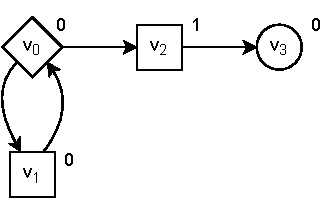
\includegraphics[scale=0.6]{Figs/inf-fixpoints-horiz.pdf}\hspace{-2ex}
\caption{A game with infinite fixpoints} \label{fig:multiple-fixpoints}
\end{wrapfigure}
\begin{example}\label{ex:several-fixpoints} Consider the (one-player) game in Fig.~\ref{fig:multiple-fixpoints}, where Player 1's vertices are drawn as boxes, Player 2's vertices are drawn as diamonds, and probabilistic vertices are depicted as circles. Note that, in that game, the greatest fixpoint is $(1,1,1,0)$.  Yet, $(0.5,0.5,1,0)$ is also a fixpoint as $\Gamma(0.5,0.5,1,0) = (0.5,0.5,1,0)$.  In fact, the Bellman operator for this game has infinite fixpoints: any $f$ of the form $(x,x,1,0)$ with $x\in[0,1]$.
\end{example}

Thus, the standard approach cannot be used here. Instead, we use the greatest fixpoint for proving determinacy, but this cannot be done directly on $\StandardBellman$.  A main difficulty is that the Knaspter-Tarski theorem does not apply for $\StandardBellman$ since $(\mathbb{R}^V, \leq)$ is not a complete lattice.  Using instead the extended reals ($(\mathbb{R} \cup \{\infty\})^V$) is not a solution, as in some cases the greatest fixpoint will assign $\infty$ to some vertices (e.g., $(\infty,\infty,0)$ would be the greatest fixpoint in the Markov chain of Fig.~\ref{fig:overflow}).
One possible approach is to approximate the greatest fixpoint from an estimated upper bound via value iteration.  Unfortunately, there may not be an order relation between $f$ and $\StandardBellman(f)$ and it may turn out that for some vertex $v$, $\StandardBellman(f)(v)>f(v)$  before converging to the fixpoint. This is shown in the next example.

\begin{wrapfigure}[7]{r}{36mm}
\vspace{-6ex}
\centering
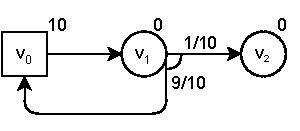
\includegraphics[scale=0.6]{Figs/overflow-horiz.pdf}\hspace{-2ex}
\caption{A game where value Iteration may go up.} \label{fig:overflow}
\end{wrapfigure}
\begin{example}\label{ex:overflow}  Consider the game depicted in Fig.~\ref{fig:overflow}.
The (unique) fixpoint in this case is $(100,90,0)$. Observe that,  we have that $\StandardBellman(120,100,0) = (110, 108, 0)$, thus the value at $v_1$ increases after one iteration. Several iterations are needed then to reach the greatest fixpoint.  Thus, in general, starting value iteration from an estimated upper bound does not guarantee  a monotone convergence to the greatest fixpoint.
\end{example}

    We overcome the aforementioned  issues by using a modified version of $\StandardBellman$. Roughly speaking, we  modify the Bellman operator in such a way that it operates over a complete lattice. 

   Notice that,  by Theorem~\ref{th:memoryless-strat-p2-bounded-expectation}, the value $\Expect{\strat{1}}{\strat{2}}_{\StochG,v}[\Rewards]$ is finite 
for every stopping game under fairness $\StochG$ and strategies $\strat{1} \in \DetMemorylessStrats{1}$, $\strat{2} \in \DetMemorylessFairStrats{2}$. 
 Furthermore, because the number of deterministic memoryless strategies is finite,  we also have that the number 
 $\max \{ \inf_{\strat{2} \in \DetMemorylessFairStrats{2}}  \sup_{\strat{1} \in \DetMemorylessStrats{1}} \Expect{\strat{1}}{\strat{2}}_{\StochG,v}[\Rewards] \mid v \in V \}$ is well defined.  
      From now on,  fix a number $\UpperBound \geq \max \{ \inf_{\strat{2} \in \DetMemorylessFairStrats{2}}  \sup_{\strat{1} \in \DetMemorylessStrats{1}} \Expect{\strat{1}}{\strat{2}}_{\StochG,v}[\Rewards] \mid v \in V \}$. We define a modified Bellman operator
$\Bellman: [0,\UpperBound]^V \rightarrow  [0,\UpperBound]^V$ as follows.
\[
    \Bellman(f)(v) =
    \begin{cases}
          \min \big( \reward(v) + \sum_{v' \in \post(v)} \delta(v,v')  f(v'),  \ \UpperBound \ \big ) & \text{ if } v \in V_\Probabilistic \setminus T  \\
          \min\big( \max\{\reward(v)  + f(v') \mid v' \in \post(v) \}, \ \UpperBound  \ \big)& \text{ if } v \in  V_1 \setminus T, \\
          \min\big( \min\{\reward(v)  + f(v') \mid v' \in \post(v) \}, \ \UpperBound \ \big) & \text{ if } v \in  V_2 \setminus T, \\
           0 & \text{ if } v \in T.
    \end{cases}
\]
%% \[
%%     \Bellman(f)(v) =
%%     \begin{cases}
%%            \reward(v) + \sum_{v' \in \post(v)} \delta(v,v')  f(v') & \text{ if } v \in V_\Probabilistic  \\
%%           \min(\mathit{opt}_{\max}(f)(v), \mathbf{U} )& \text{ if } v \in  V_1 \setminus T, \\
%%           \min( \mathit{opt}_{\min}(f)(v), \textbf{U}) & \text{ if } v \in  V_2 \setminus T, \\
%%            0 & \text{ if } v \in T.
%%     \end{cases}
%% \]
%% where:
%% $
%%     \mathit{opt}_{\oplus}(f)(v) =  \oplus \{\reward(v)  + f(v') \mid v' \in \post(v) \}
%% $
%% and $\oplus \in \{\min, \max\}$.
%\[
%\mathit{opt}_{\min}(f)(v) =  \min \{\reward(v)  + f(v') \mid v' \in \post(v) \}.
%\]
Note that $\Bellman$ is monotone, which can be proven by observing that maxima, minima and convex combinations are all monotone operators.  
Furthermore, $\Bellman$ is also Scott continuous (it preserves suprema of directed sets), this can be proven similarly as in \cite{DBLP:conf/memics/BrazdilKN12}. The following theorem 
formalizes these properties. A detailed proof can be found in the Appendix.
%\remarkPC{Podemos agregar una peque\~na discusion de por que la funci\'on tiene varios puntos fijo, quizas un ejemplo?}
\begin{theorem}\label{th:continuity} $\Bellman$ is monotone and Scott-continuous.
\end{theorem}
Note that $([0,\UpperBound]^V, \leq)$ is a complete lattice. Thus by Theorem \ref{th:continuity} and the Knaster-Tarski theorem  \cite{davey1990introduction}., the (non-empty) set of fixed points of $\Bellman$ forms a complete lattice, and the greatest fixpoint of the operator can be approximated by successive  applications of $\Bellman$ to the top element (i.e., $\UpperBound$) \cite{davey1990introduction}. In the following we denote by $\nu \Bellman$ the greatest fixed point of $\Bellman$.

%The following theorem states that game determinacy is preserved when Player 2 is restricted to play fair strategies.
The following theorem states that games restricted to fair strategies on Player~2 are determinate.
Furthermore, the value of the game is given by the greatest fixpoint of $\Bellman$.
\begin{theorem}\label{th:game-determinacy} Let $\StochG$ be a stochastic game  that is stopping under fairness. It holds that:
\[\adjustlimits
	\inf_{\strat{2} \in \FairStrats{2}} \sup_{\strat{1} \in \Strategies{1}} \Expect{\strat{1}}{\strat{2}}_{\StochG,v}[\Rewards] = \adjustlimits \sup_{\strat{1} \in \Strategies{1}}   \inf_{\strat{2} \in \FairStrats{2}}  \Expect{\strat{1}}{\strat{2}}_{\StochG,v}[\Rewards] = \nu \Bellman(v)
\]
\end{theorem}
%
\begin{proof}
  First, note that   $\inf_{\strat{2} \in \DetMemorylessFairStrats{2}}  \sup_{\strat{1} \in \DetMemorylessStrats{1}} \Expect{\strat{1}}{\strat{2}}_{\StochG,v}[\Rewards]$
  is a fixed point of $\Bellman$.  Thus we have:
   \begin{align*}	
       % \label{th:game-determinacy-eq1-l1}
        \adjustlimits \sup_{\strat{1} \in \Strategies{1}}   \inf_{\strat{2} \in \FairStrats{2}}  \Expect{\strat{1}}{\strat{2}}_{\StochG,v}[\Rewards]
        & \leq \adjustlimits \inf_{\strat{2} \in \FairStrats{2}} \sup_{\strat{1} \in \Strategies{1}} \Expect{\strat{1}}{\strat{2}}_{\StochG,v}[\Rewards] \\
      % \label{th:game-determinacy-e1-l2}
        &   \leq \adjustlimits  \inf_{\strat{2} \in \DetMemorylessFairStrats{2}}  \sup_{\strat{1} \in \DetMemorylessStrats{1}} \Expect{\strat{1}}{\strat{2}}_{\StochG,v}[\Rewards] 
         \leq   \nu \Bellman(v) 
  \end{align*} 
  %First, note that $\inf_{\strat{2} \in \FairStrats{2}} \sup_{\strat{1} \in \Strategies{1}} \Expect{\strat{1}}{\strat{2}}_{\StochG,v}[\Rewards]$ is a fixed point of $\Gamma$. 
  %Thus we have:
  %\[
  %\adjustlimits
  %\sup_{\strat{1} \in \Strategies{1}}   \inf_{\strat{2} \in \FairStrats{2}}  \Expect{\strat{1}}{\strat{2}}_{\StochG,v}[\Rewards]
  %\leq 
  %\adjustlimits \inf_{\strat{2} \in \FairStrats{2}} \sup_{\strat{1} \in \Strategies{1}} \Expect{\strat{1}}{\strat{2}}_{\StochG,v}[\Rewards]
  %\leq
  %\inf_{\strat{2} \in \DetMemorylessFairStrats{2}}  \sup_{\strat{1} \in \DetMemorylessStrats{1}} \Expect{\strat{1}}{\strat{2}}_{\StochG,v}[\Rewards]
  %\leq
  %\nu \Gamma(v)
  %\]
  for any $v$. The first inequality is a standard property of suprema and infima \cite{Kucera2011}, the second inequality holds because  
  $\DetMemorylessFairStrats{2} \subseteq \FairStrats{2}$ and standard properties of MDPs: by fixing a deterministic memoryless  
  fair strategy for Player $2$ we obtain a transient MDP, the optimal strategy for Player $1$ in this MDP is obtained via a deterministic memoryless strategy \cite{Kallenberg83}. The last inequality holds because  $\inf_{\strat{2} \in \DetMemorylessFairStrats{2}}  \sup_{\strat{1} \in \DetMemorylessStrats{1}} \Expect{\strat{1}}{\strat{2}}_{\StochG,v}[\Rewards]$ is 
  a fixpoint of $\Bellman$. 
  
  Rest to prove that $\sup_{\strat{1} \in \Strategies{1}}   \inf_{\strat{2} \in \FairStrats{2}}  \Expect{\strat{1}}{\strat{2}}_{\StochG,v}[\Rewards] \geq \nu \Bellman(v)$. Note that, if there is  $\strat{1} \in \Strategies{1}$ such that
  $\inf_{\strat{2} \in \FairStrats{2}}  \Expect{\strat{1}}{\strat{2}}_{\StochG,v}[\Rewards] \geq \nu \Bellman(v)$ the property above follows by properties of supremum. Consider the strategy $\starredstrat{1}$ defined as follows:
  $\starredstrat{1}(v) \in \argmax \{\nu \Bellman(v') + \reward(v) \mid v' \in \post(v) \}$. Note that $\starredstrat{1}$ is a memoryless and deterministic strategy. For any memoryless, deterministic and fair strategy $\strat{2} \in \DetMemorylessFairStrats{2}$ we have
  $\nu \Bellman(v) \leq \Expect{\starredstrat{1}}{\strat{2}}_{\StochG,v}[\Rewards]$ (by definition of $\Bellman$).  Thus,
  %
  $\nu \Bellman(v) \leq \inf_{\strat{2} \in \DetMemorylessFairStrats{2}} \Expect{\starredstrat{1}}{\strat{2}}_{\StochG,v}[\Rewards]$
  %
  and therefore:
  %
  $\nu \Bellman(v) \leq \sup_{\strat{1} \in \DetMemorylessStrats{1}} \inf_{\strat{2} \in \DetMemorylessFairStrats{1}} \Expect{\strat{1}}{\strat{2}}_{\StochG,v}[\Rewards]$.
  %
  Finally, by Theorem \ref{th:reduce-to-memoryless} we get:
  %
  $\nu \Bellman(v) \leq \sup_{\strat{1} \in \Strategies{1}} \inf_{\strat{2} \in \FairStrats{2}} \Expect{\strat{1}}{\strat{2}}_{\StochG,v}[\Rewards]$.
  \qed
\end{proof}
%
%\subsection{Considerations for an algorithmic solution}
\paragraph{Considerations for an algorithmic solution.}
Value iteration \cite{Bellman57} has been used to compute maximum/minimum expected accumulated reward in MDPs, e.g., in the {\Prism} model checker.  Usually, the value is computed by approximating the least fixpoint from below using the Bellman equations \cite{Bellman57}. In~\cite{DBLP:conf/cav/Baier0L0W17}, the authors propose to approach these values from both a lower and an upper bound (known as interval iteration \cite{DBLP:journals/tcs/HaddadM18}). To do so,  \cite{DBLP:conf/cav/Baier0L0W17} shows a technique for computing upper bounds for the expected total rewards for MDPs.  This approach is based on the fact that, given a stopping MDP $\StochG$, $\ExpectMDP{\strat{1}}_{\mathcal{G},v}[\Rewards] = \sum_{v' \in R(v)} \zeta_v^{\strat{1}}(v')*\reward(v')$,  where $R(v)$ denotes the set of reachable states from $v$, and $\zeta_v^{\strat{1}}(v')$ denotes the  expected number of times to visit $v'$ in the Markov chain
induced by $\strat{1}$ when starting at $v$.  \cite{DBLP:conf/cav/Baier0L0W17} describes how to compute  a value $\zeta_{v}^*(v')$, such that $\zeta_v^*(v') \geq \sup_{\strat{1} \in \Strategies{1}} \zeta_v^{\strat{1}}(v')$. Thus,  $\sum_{v' \in R(v)} \zeta_v^{*}(v')*\reward(v')$ gives an upper bound for $\sup_{\strat{1}} \ExpectMDP{\strat{1}}_{\mathcal{G},v}[\Rewards]$.  
\begin{wrapfigure}[12]{r}{0.555\textwidth}
    \vspace{-9.5ex}
    \begin{minipage}{0.55\textwidth}
      \begin{algorithm}[H]
        \caption{Algorithm for computing GFP}\label{Alg:gfp}
        \begin{algorithmic}
          \REQUIRE $\StochG$ is a stopping under fairness game\\[1ex]
          \STATE $\delta' \gets  \lambda (v,v') {.} (v \in V_1 {\cup} V_\Probabilistic) \mathop{?} \delta(v,v') : \frac{1}{|\post^{\mathcal{G}}(v)|}$\\[-1ex]
          \STATE  $\mathcal{G}' \gets (V, (V_1, \emptyset, V_2{\cup}V_\Probabilistic)), \delta')$
          \STATE $x' \gets \lambda v : \sum_{v' \in R(v)} : \zeta^*_v(v')*\reward(v')$
          \REPEAT
          \STATE $x \gets x'$
          \STATE $x' \gets \Bellman(x)$
          \UNTIL{$|| x - x' || \leq \varepsilon$}
          \RETURN $x'$
        \end{algorithmic}
      \end{algorithm}
    \end{minipage}
  \end{wrapfigure}
    Our algorithm uses these ideas to provide an upper bound for two-player games.  Roughly speaking,  the above defined functional $\Bellman$ presents a form of Bellman equations that enables a value iteration algorithm to solve these games.  We need to start with some value vector larger than such a fixpoint.  Given a stopping under fairness game,  we fix a (memoryless) fair strategy for the environment, thus obtaining an MDP.  We then use the techniques described above  to find an upper bound for this MDP, which in turn is an upper bound in the original game. The obvious fair strategy to use is the one based on the uniform distribution (as in Theorem \ref{thm:uniform-prob}).  This idea is described in Alg.~\ref{Alg:gfp}.  It is worth noting that, instead of using a unique upper bound for every vertex (as in the definition of $\Bellman$), the algorithm may use a different upper bound for each component of the value vector, this improves the number of iterations performed by the algorithm. 
We have implemented Alg.~\ref{Alg:gfp} as a prototype embedded in the {\PrismGames} toolset~\cite{DBLP:conf/cav/KwiatkowskaN0S20}, 
as described in the next section. 
%\remarkPC{Agregar un parrafo que en vez de usar $\UpperBound$, usamos un vector.}
%\remarkPRD{Por ah\'i yo dir\'ia \textbf{``We have implemented this algorithm as a prototype embedded in the {\Prism}-game toolset~\cite{DBLP:conf/cav/KwiatkowskaN0S20}.''} De cualquier manera, el paper \cite{DBLP:conf/cav/KwiatkowskaN0S20}. hay que referenciarlo }
   %    We have implemented these ideas in a prototype tool as described in the next section.


%% old text
%Value iteration \cite{Bellman57} has been used to compute maximum/minimum expected accumulated reward in MDPs, e.g. in the {\Prism} model checker.  Usually, the value is computed by approximating the least fixed point from below using the Bellman equations \cite{Bellman57}. In~\cite{DBLP:conf/cav/Baier0L0W17}, the authors propose to approach these values from both a lower and an upper bound (known as interval iteration \cite{DBLP:journals/tcs/HaddadM18}). To do so,  \cite{DBLP:conf/cav/Baier0L0W17} shows a technique for computing upper bounds for the expected total rewards for MDPs.

%The above defined functional $\Bellman$ presents a form of Bellman equations that enables a value iteration algorithm to solve our games.  As we are looking for the greatest fixed point, we need to start with some value vector larger than such a fixed point.
%
%If we take our game and fix a fair strategy for the environment, we obtain an MDP. We can then use the techniques presented in \cite{DBLP:conf/cav/Baier0L0W17} to find an upper bound in this MDP, which in turn is an upper bound in the original game. The obvious fair strategy to use is the one based on the uniform distribution (as in Theorem \ref{thm:uniform-prob}).  We have implemented these ideas in a prototype tool as described in the next section.


	
	
	

\section{Related Work} \label{sec:related_work}

Stochastic games with payoff functions have been extensively investigated in the literature. In \cite{FilarV96}, several results are presented about \emph{transient games},
a generalized version of stopping stochastic games with total reward payoff. 
In transient games, both players possess optimal (memoryless and deterministic) strategies. 
Most importantly, the games are determined and their value can be computed as the least fixed point of a set of equations. 
Most of these results are based on the fact that the $\Gamma$ functional (see Section \ref{sec:fair-strats}) for transient games has a unique fixed point.
Notice that in this paper we have dealt with games that are stopping only under fairness assumptions. Thus, the corresponding functional 
may have several fixed points. Hence, the main results presented in \cite{FilarV96} do not apply to our setting.


\cite{DBLP:journals/fmsd/ChenFKPS13} and \cite{SvorenovaKwiatkowska16} present logical frameworks for the verification and synthesis of systems.  While~\cite{DBLP:journals/fmsd/ChenFKPS13} provides a solution for a  probabilistic branching temporal logic extended with expected total, discounted, and average reward objective functions, \cite{SvorenovaKwiatkowska16} does the same in a similar extension of a probabilistic linear temporal logic. Both frameworks were implemented in the tool \Prism~\cite{DBLP:conf/cav/KwiatkowskaN0S20,DBLP:conf/cav/KwiatkowskaNP11}.  Although a vast class of properties can be expressed in these frameworks, none of them are presented under fair environments.  In fact, these works are on stochastic multiplayer games in which each player is treated equally.
%% \cite{DBLP:journals/fmsd/ChenFKPS13} and \cite{SvorenovaKwiatkowska16} present logical frameworks for the verification and synthesis of systems.  While~\cite{DBLP:journals/fmsd/ChenFKPS13} presents a framework that combines a probabilistic branching temporal logic with expected total, discounted, and average reward objective functions, \cite{SvorenovaKwiatkowska16} does the same in the context of a probabilistic linear temporal logic. Both frameworks were implemented in the tool \Prism~\cite{DBLP:conf/cav/KwiatkowskaNP11}. Although a vast class of properties can be expressed in these frameworks, none of them are presented under fair environments.  In fact, these works are on stochastic multiplayer games in which each player is treated equally.

However, of all the operators in~\cite{DBLP:journals/fmsd/ChenFKPS13,SvorenovaKwiatkowska16,DBLP:conf/cav/KwiatkowskaN0S20}, $\langle \langle p_1 \rangle \rangle \ \textsf{R}_{\text{max}{=}?}[\textsf{F}^{\infty} T]$ is the closest to our proposal and it deserves a deeper comparison.  $\langle \langle p_1 \rangle \rangle \ \textsf{R}_{\text{max}{=}?}[\textsf{F}^{\infty} T]$ returns the expected accumulated reward until reaching $T$ in which infinite plays receive an infinite value~\cite{DBLP:journals/fmsd/ChenFKPS13,DBLP:conf/cav/KwiatkowskaN0S20}.
{\Prism} approximates this value by computing a greatest fixpoint.  It uses a two-phase algorithm to do so:
\begin{enumerate}[(i)]
\item%
  it first replaces zero rewards with a small positive value and applies value iteration on this modification to get an estimated upper bound, and
\item%
  this upper bound is used to start another value iteration process aimed to compute the greatest fixpoint.
\end{enumerate}
%
\begin{wrapfigure}[10]{r}{55mm}
\vspace{-4ex}
%\fontsize{6.6}{6.6}\selectfont\ttfamily
\centering
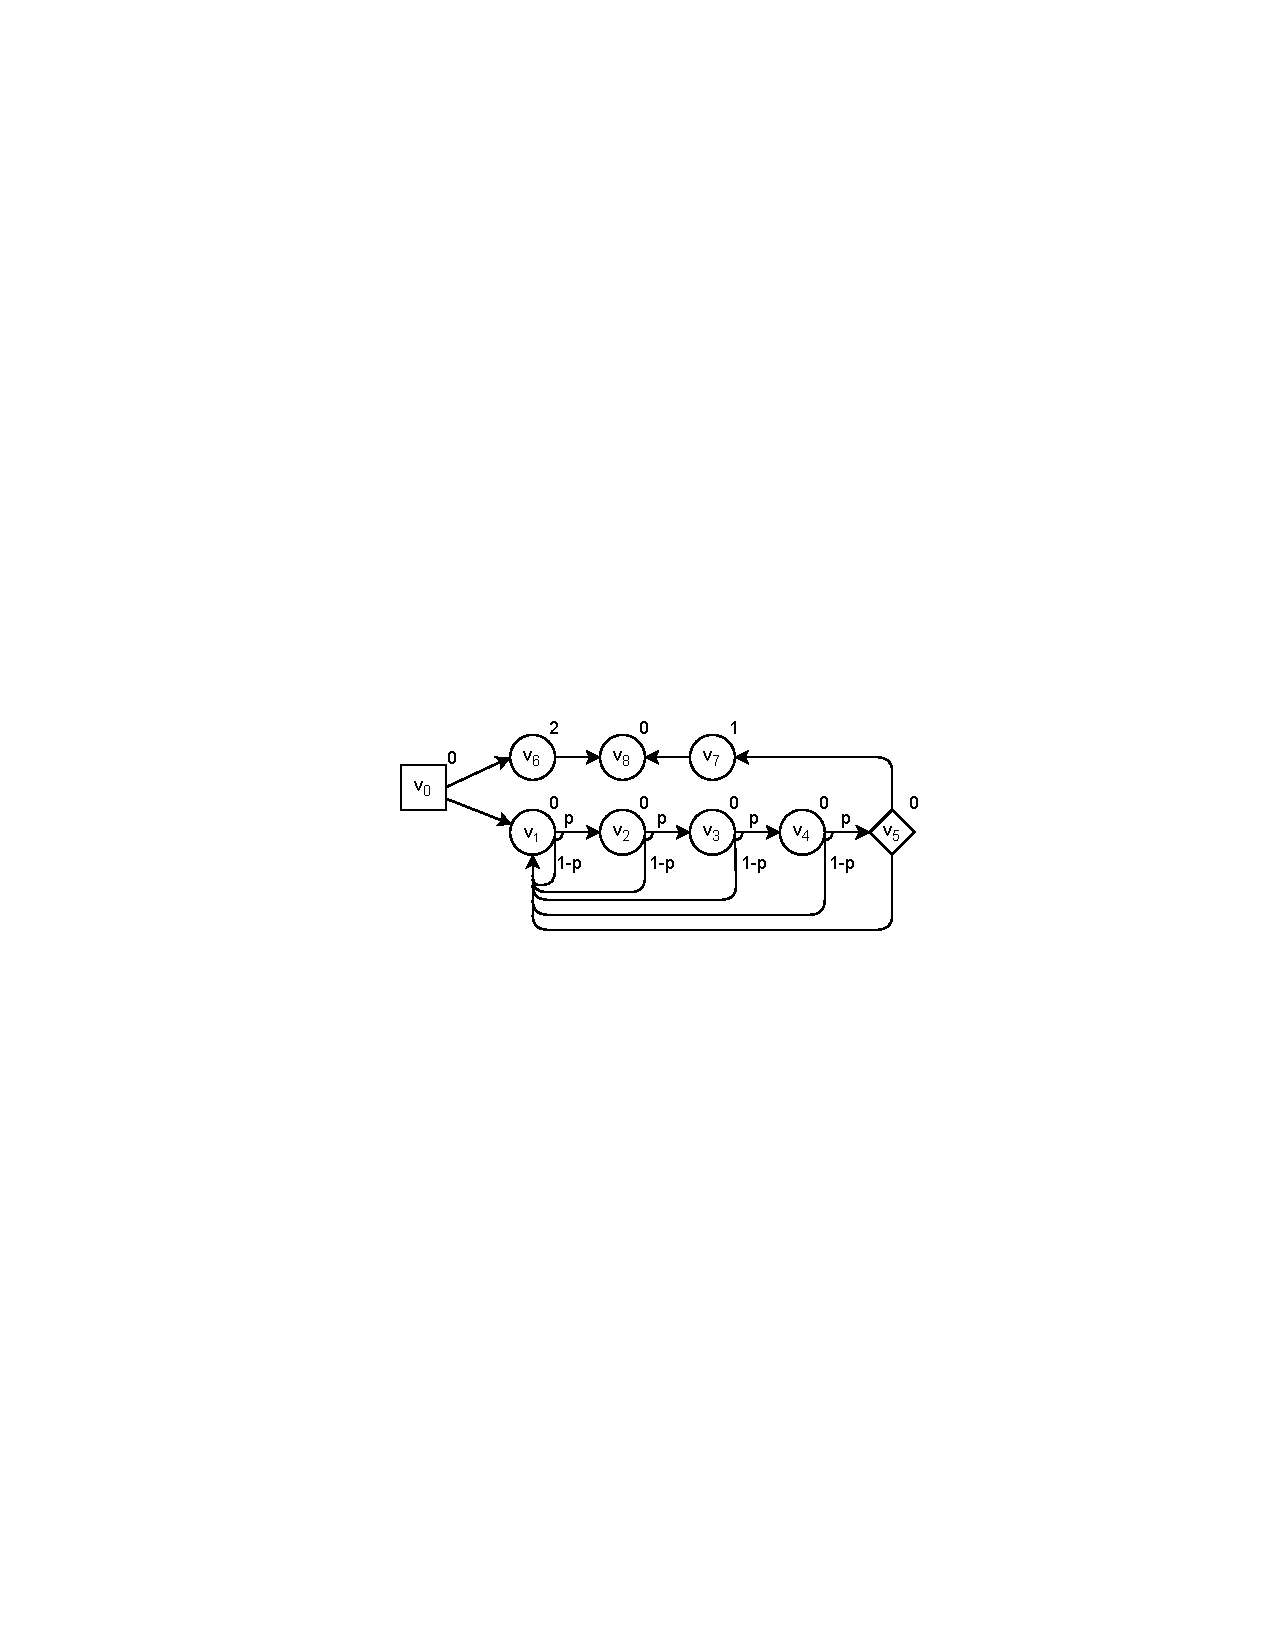
\includegraphics[scale=0.60]{Figs/prism-cex-1-horiz.pdf}%\hspace{1.5em}\mbox{}
\caption{A simple 2-player game: only probability less than 1 are shown.} \label{fig:prism-cex-1}
\end{wrapfigure}
This heuristic could return erroneous approximations of the greatest fixpoint.  We illustrate this with a simple example. Consider  the game depicted in Fig.~\ref{fig:prism-cex-1}, For any $\textsf{p}$, the value of the greatest fixpoint in vertex $v_0$ is $2$. However, by taking $\textsf{p}=0.99$ and tolerance $\epsilon=10^{-6}$, {\Prism} returns a value close to $39608$. %the value $39607.955145476146$.
This occurs because  {\Prism} changes $0$ to the value $0.02$, which results in an extremely large upper bound.
%% Furthermore, every iteration only produces a small modification in the values %which yields an erroneous final value
%% which leads to an incorrect convergence.
Obviously, it also returns an incorrect strategy for vertex $v_0$.  We have checked this example with our tool, and it returned the correct value for vertex $v_0$ in $2$ iterations, regardless of the value of $\textsf{p}$.
%
We have chosen a large value for $\textsf{p}$ to make the difference noticeable. Small values also may produce different values in, e.g., $\textsf{v}_1$ only that it could be blamed on approximation errors.
%
%% Varying the relative error does not yield a better solution. In fact, taking $\epsilon = 10^{-8}$ {\Prism} returns a value closer to $2010051$.
%% \remarkPRD{Saque lo de las iteraciones porque no creo que agregue nada}
%% %a value of $2010050.7754585734$,  and also the number of iterations needed to compute such a value is increased: {\Prism} took $69508550$ iterations and $~30$ seconds with $\epsilon=10^{-8}$.}
%% Similar examples can be built to show that the upper bound estimated by {\Prism} could return a value smaller than the greatest fixpoint, yielding an incorrect final value.
%
We have also run this operator on our case studies and observed small differences in many of them (particularly on Roborta) that get larger when the fault probabilities get larger as well.%\remarkPRD{Verificar esta \'ultima oraci\'on que la estroy poniendo por un comentario de Pablo} 



%% \paragraph{{\Prism} Operators.} {\Prism} supports 2-player stochastic games,  therein properties are specified via the logic $\text{rPATL}$.This logic provides operators for expected rewards. Most of these operators are computed via a least fixpoint; thus, they are not comparable with our approach (they return $0$ in the case of a $0$-valued cycles).
%% Interestingly,  the operator  $\langle \langle p_1 \rangle \rangle \ \textsf{R}_{\text{max}{=}?}[\textsf{F}v]$ \remarkPRD{cambi\'e esto. Antes dec\'ia $\langle \langle p_1 \rangle \rangle \text{min}{=}?\textsf{R}[\textsf{F}v]$. Fijense que cambi\'e ``min'' por ``max''} returns the expected accumulated reward in which infinite plays receive an infinite value~\cite{DBLP:journals/fmsd/ChenFKPS13,DBLP:conf/cav/KwiatkowskaN0S20}.  {\Prism} approximates this value by computing a greatest fixpoint.  It uses a two-phase algorithm to do so:
%% \begin{enumerate}[(i)]
%% \item%
%%   it first replaces $0$-rewards by a small positive value and applies value iteration on this modification to get an estimated upper bound, and
%% \item%
%%   this upper bound is used to start another value iteration process aimed to compute the greatest fixpoint.
%% \end{enumerate}
%% %
%% \begin{wrapfigure}[10]{r}{55mm}
%% \vspace{-4ex}
%% %\fontsize{6.6}{6.6}\selectfont\ttfamily
%% \centering
%% 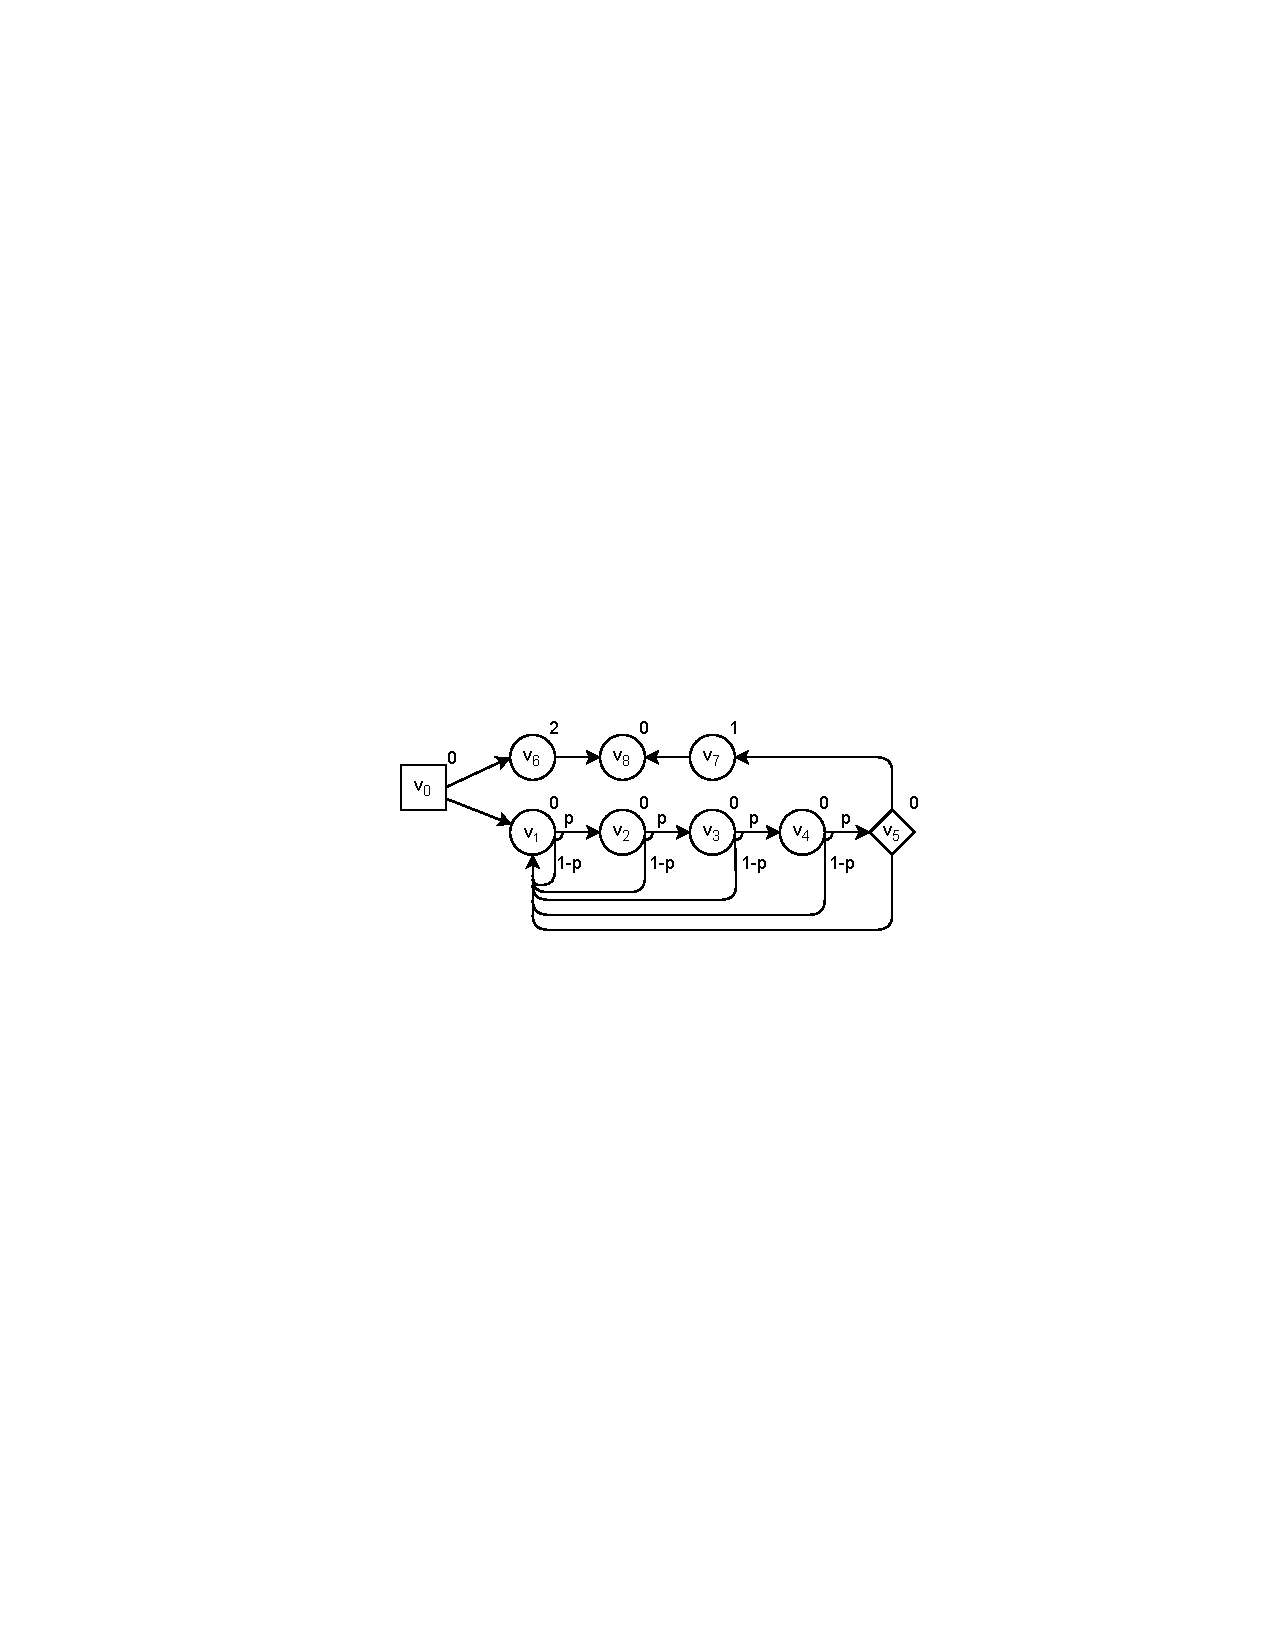
\includegraphics[scale=0.60]{Figs/prism-cex-1-horiz.pdf}%\hspace{1.5em}\mbox{}
%% \caption{A simple 2-player game: only probability less than 1 are shown.} \label{fig:prism-cex-1}
%% \end{wrapfigure}
%% This heuristic could return erroneous approximations of the greatest fixpoint.  We illustrate this with a simple example. Consider  the game depicted in Fig.~\ref{fig:prism-cex-1}, For any $T$, the value of the greatest fixpoint in vertex $v_0$ is $2$. However, by taking $T=0.99$ and tolerance $\epsilon=10^{-6}$, {\Prism} returns a value close to $39608$. %the value $39607.955145476146$.
%% This occurs because  {\Prism} changes $0$ by the value $0.02$, which results in an extremely large upper bound.  Furthermore, every iteration only produces a small modification in this value which yields an erroneous final value which leads to an incorrect convergence.   Obviously, it also returns an incorrect strategy for vertex $v_0$.  We have checked this example with our tool, and it returned the correct value for  vertex $v_0$ in $2$ iterations.
%% %
%% Varying the relative error does not yield a better solution. In fact, taking $\epsilon = 10^{-8}$ {\Prism} returns a value closer to $2010051$.
%% \remarkPRD{Saque lo de las iteraciones porque no creo que agregue nada}
%% %a value of $2010050.7754585734$,  and also the number of iterations needed to compute such a value is increased: {\Prism} took $69508550$ iterations and $~30$ seconds with $\epsilon=10^{-8}$.}
%% Similar examples can be built to show that the upper bound estimated by {\Prism} could return a value smaller than the greatest fixpoint, yielding an incorrect final value.


















	\emph{Stochastic shortest path games} \cite{PatekBertsekas99} are two-player stochastic games with (negative or positive) rewards in which the minimizer's strategies are classified into \emph{proper} and \emph{improper},
proper strategies are those ensuring termination.  As proven in \cite{PatekBertsekas99}, these games are determined, and both players posses memoryless optimal strategies.  To prove these results,  the authors assume that the expected game value for improper strategies is $\infty$, this ensures that the corresponding functional is a contraction and thus it has a unique fixpoint. In contrast, we restrict ourselves to non-negative rewards but we do not make any assumptions over unfair strategies, as mentioned above the corresponding functional for our games may have several fixpoints. Furthermore, we proved that the value of the game is given by the greatest fixpoint of $\Gamma$.  In recent years, several authors have investigated stochastic shortest path problems for MDPs (i.e,  one-player games), where the assumption over improper strategies  is relaxed (e.g., \cite{DBLP:conf/lics/Baier0DGS18}); to the best of our knowledge, these results have not be extended to two-player games.  

%% In \cite{SvorenovaKwiatkowska16}, a logical framework is presented for the verification and synthesis of systems. This framework combines probabilistic linear temporal logic with expected total, discounted, and average reward objective functions. 	The framework is implemented in the tool \Prism~\cite{DBLP:conf/cav/KwiatkowskaNP11}. Although a vast class of properties can be expressed in this framework, fairness assumptions over the environment are not dealt with in this line of research.
	
	In \cite{DBLP:conf/ifipTCS/BolligC04} the authors tackle the problem of synthesizing a controller that maximizes the probability of satisfying an {\LTL} property. Fairness strategies are used to reduce this problem to the synthesis of a  controller maximizing a {\PCTL} property over a product game. However, this article does not address expected rewards and game determinacy under fairness assumptions. 
	
	Interestingly, in \cite{DBLP:conf/fossacs/AsarinCV10} the authors consider the problem of winning a (non-stochastic) two-player games with fairness assumptions over the environment. The objective of the system is to guarantee an $\omega$-regular property. The authors show that winning in these games is equivalent to almost-sure winning in a Markov decision process. It must be noted that this work only considers non-stochastic games.  Furthermore, payoff functions are not considered therein.
%% Interestingly, in \cite{DBLP:conf/fossacs/AsarinCV10} the authors consider the problem of winning a (non-stochastic) two-player games with fairness assumptions over the environment. The objective of the system is to guarantee an $\omega$-regular property. The authors show that winning in these games is equivalent to almost-sure winning in a Markov decision process. It must be noted the aforementioned work only considers non-stochastic two-player games.  Furthermore, payoff functions are not considered therein.


        
%	The games introduced in \cite{Bacci0LM17,BacciBLMTB19,DesharnaisGJP04,DesharnaisLT11}  are based on probabilistic bisimulation, so they are symmetric. Furthermore, in \cite{DesharnaisGJP04,DesharnaisLT11} the nodes of the game graph are modeled using subsets of states of the PTSs, in our formulation
%we do not use subsets of states. The games defined in \cite{Bacci0LM17,BacciBLMTB19} use Kanterovich's and Hausdorff's liftings to deal with probabilistic distributions and non-determinism, respectively. In addition, the authors use the vertices of the transportation polytopes to model the probabilistic vertices. In contrast, we introduced a symbolic representation of games to avoid the state explosion caused by the vertices of the polytopes. Also note that the metrics introduced in \cite{Bacci0LM17,BacciBLMTB19} measure the (probabilistic) bisimulation distance between two PTSs, which for almost-sure failing systems is always $1$.
%		
%Another related framework is  defined in \cite{LanotteMT17}. Therein, the authors introduce a notion of weak simulation quasimetric tailored for reasoning about the evolution of \emph{gossip protocols}. This makes possible to compare network protocols that have similar behaviour up to a certain tolerance; being $0$ and $1$ the minimum and maximum distance, respectively.  Note that using this quasimetric to compare a network protocol with an almost-sure failing implementation will always return $1$, thus that approach cannot be used to quantify the masking fault-tolerance of almost-sure failing systems.
% 
% Finally, let us compare our approach with some metrics usual in fault-tolerance. \emph{Mean-Time To Failure} (MTTF) and \emph{Mean-Time Between Failures} (MTBF) \cite{ReliabilityBook}  capture the amount of time that a system is expected to be operative until it fails, and the expected elapsed time between failures, respectively.  These metrics are designed for hardware or electronic systems, where we have at hand estimations about the failure rate of the physical components. Our framework is designed to be used at a higher level of abstraction, where we have a model of the system to be implemented acting as a specification, and several possible implementations of it, described as probabilistic automata. This level of abstraction makes it possible to use this framework to analyze software fault-tolerance. Furthermore, note that our framework is particularly tailored to deal with masking fault-tolerance, a particular kind of fault-tolerance; in addition, our game formulation allows us to analyse systems on worst-case scenarios.

%\spnewtheorem*{proofofclaim}{Proof of claim}{\itshape}{\rmfamily}
\newenvironment{myproof}[1][]{\begingroup\renewcommand{\proofname}{\textbf{Proof #1}}\begin{proof}}{\end{proof}\endgroup}


\section{Proofs}\label{sec:appendix}


\begin{myproof}[of Lemma~\ref{lemma:memoryless-strat}]
  Fix strategies $\strat{1} \in \Strategies{1}$, $\strat{2} \in
  \FairStrats{2}$ and a vertex $v \in V$ such that
  $\Prob{\strat{1}}{\strat{2}}_{\mathcal{G}, v}(\Diamond T) < 1$.
  Note that we can define an MDP (named $\StochG^{V_1{+}V_2}$) from
  $\StochG$ by considering that $V_1$ and $V_2$ belong to the same
  player.  For this MDP consider the set $U = \{ (V',\delta')
  \mid(V',\delta') \in \EndComp(\StochG^{V_1{+}V_2}) \text{ and }
  V'\cap T = \emptyset \}$ of end components not containing terminal
  vertices.  So, we define a strategy for this player combining
  $\strat{1}$ and $\strat{2}$ (named $\strat{1}{+}\strat{2}$) as
  follows: it behaves as $\strat{1}$ in finite paths ending in a state
  of $V_1$, and behaves as $\strat{2}$ in finite paths ending in a
  state of $V_2$. Note that we have
  $\MDPProb{\strat{1}{+}\strat{2}}_{\StochG^{V_1+V_2},v}(\Diamond T) <
  1$. By the limit properties of MDPs (Theorem 10.120 \cite{BaierK08})
  we have that:
  %
  \begin{equation}\label{lemma:memoryless-strat-eq1}
    \MDPProb{\strat{1}{+}\strat{2}}_{\StochG^{V_1+V_2},v} \left(\{ \omega \in \MDPPaths{\strat{1}{+}\strat{2}}_{\StochG^{V_1+V_2},v} \mid \limit(\omega)  \in U \}\right) > 0,
  \end{equation}
  %
  where $\limit(\omega)$ denotes the end-component that is repeated
  infinitely often in $\omega$, as defined in \cite{BaierK08}.  Note
  that, the fairness of $\strat{2}$ and
  (\ref{lemma:memoryless-strat-eq1}) imply that there is a reachable
  end component $\EC{C}= (V',\delta') \in U$ such that, for all
  $v' \in V_2 \cap V'$, $\post^\delta(v') \subseteq V'$ $(\dag)$.
  %
  This
  can be proven by contradiction: if $(\dag)$ does not hold we have
  that for every end component in $U$ there must be some vertex in
  $V_2$ such that some of its successors is not in the component; but,
  since $\strat{2}$ is fair, we should have
  %
  $\MDPProb{\strat{1}{+}\strat{2}}_{\StochG^{V_1+V_2},v} \left ( \{ \omega \in \MDPPaths{\strat{1}{+}\strat{2}}_{\StochG^{V_1+V_2},v} \mid \limit(\omega) \in U \}\right) = 0$
  %
  contradicting (\ref{lemma:memoryless-strat-eq1}). Thus $(\dag)$ must hold.

  Hence, there is some finite path $\hat{\omega} = v_0 v_1 v_2 \dots v_k$
  in this MDP such that $v_i \notin T$ for every $i$, $v_k \in V'$, and
  $\MDPProb{\strat{1}{+}\strat{2}}_{\StochG^{V_1+V_2},v}(v_0\dots v_k) > 0$.

  Now, we define $\strat{1}'$ as follows:
  %
  $\strat{1}'(v') = \hat{\omega}_{i+1}$, if $i < k$ is the largest
  index such that $v' = \hat{\omega}_{i}$;
  %
  $\strat{1}'(v') = v''$ for some arbitrary $v'' \in
  V'\cap\post^\delta(v)$, if $v' \in V'$;
  %
  otherwise $\strat{1}'(v') = v''$ for some arbitrary
  $v'' \in \post^\delta(v')$.
  %
  $\strat{2}'$ is defined as the uniform strategy, that is:
  $\strat{2}'(v')(v'') = \frac{1}{\# \post^\delta(v')}$, for every $v'
  \in V_2$ and $v'' \in \post^\delta(v')$.
  
  $\strat{1}'$ is defined such that it jumps ahead on $\hat{\omega}$
  skipping all possible loops introduced by $\strat{1}$.  Let
  $\hat{\omega}{\downharpoonleft}_{\strat{1}'}$ be the finite path
  obtained by following $\hat{\omega}$ skipping all loops according
  to $\strat{1}'$.
  %
  Note that $\hat{\omega}{\downharpoonleft}_{\strat{1}'}$ is a valid
  path in $\StochG$, that it still ends in state $v_k$, and that
  $\MDPProb{\strat{1}',\strat{2}'}_{\StochG,v}({\hat{\omega}{\downharpoonleft}_{\strat{1}'}})>0$.
  Moreover, by ($\dag$) and the definition of $\strat{1}'$, we have
  that $\MDPProb{\strat{1}',\strat{2}'}_{\StochG, v_k}(\Box V') = 1$.
  Thus $\MDPProb{\strat{1}',\strat{2}'}_{\StochG, v}(\Diamond T) < 1$.
  Furthermore, note that $\strat{1}'$ is memoryless and $\strat{2}'$
  is fair.
%%   Now, we define $\strat{1}'$ as follows: $\strat{1}'(v') = \hat{\omega}_{i+1}$, if $v' = \hat{\omega}_{i}$ for some $i <k$; 
%% $\strat{1}'(v') = v''$ for some arbitrary $v'' \in \post^\delta(v')$, if $v' \neq \hat{\omega}_{i}$ for all $i \leq k$ and $v' \notin V'$; $\strat{1}'(v') = v''$ for some arbitrary $v'' \in V'\cap \post^\delta(v)$, if
%% $v' \in V'$. $\strat{2}'$ is defined as the uniform strategy, that is: $\strat{2}'(v')(v'') = \frac{1}{\# \post^\delta(v')}$, for every $v' \in V_2$ and $v'' \in \post^\delta(v')$. Note that, $\MDPProb{\strat{1}',\strat{2}'}_{\StochG,v}(v_0\dots v_k) >0$, and 
%% also (by definition of $\strat{1}'$ and ($\dag$)) we have that $\MDPProb{\strat{1}',\strat{2}'}_{\StochG, v_k}(\Box V') = 1$, thus $\MDPProb{\strat{1}',\strat{2}'}_{\StochG, v}(\Diamond T) < 1$. Furthermore, note that $\strat{1}'$ is memoryless and $\strat{2}'$ is fair.%we can define strategies
%% %$\strat{1}'$ and $\strat{2}'$ such that they collaborate to reach $\EC{C}$, and for any vertex $\hat{v} \in V_1 \cap V'$ we set 
%% %$\strat{1}'(\hat{v})=v'$ (for some $v' \in V'$); while $\strat{2}'$ behaves as $\strat{2}$ in nodes belonging to $V_2$. Note that this
%% %ensures that $\strat{2}'$ is fair and $\strat{1}'$ is memoryless. Since the probability of reaching $\EC{C}$ is positive, and no node in $T$ is reached when playing $\strat{1}'$ and $%\strat{2}'$,  we get that $\Prob{\strat{1}'}{\strat{2}'}_{\StochG, v}(\Diamond T) < 1$.
\qed
\end{myproof}


\begin{myproof}[of Theorem~\ref{thm:uniform-prob}]
``If'': Suppose that $\Prob{\strat{1}}{\uniformstrat{2}}_{\StochG,v}(\Diamond T)=1$ for every Player~1's strategy $\strat{1}$.  Moreover, 
assume, for the sake of contradiction, that
$\Prob{\strat{1}'}{\strat{2}'}_{\StochG,v}(\Diamond T) < 1$ for some  $\strat{1}'\in \Strategies{1}$ and $\strat{2}'\in \FairStrats{2}$. 
By Lemma \ref{lemma:memoryless-strat}, we can safely assume that $\strat{1}'$ is memoryless and deterministic.
Thus, by fixing $\strat{1}'$, we obtain a (finite) Markov decision process denoted $\StochG^{\strat{1}'}$.
By assumption, we have that
$\inf_{\strat{2} \in \FairStrats{2}} \MDPProb{\strat{2}}_{\StochG^{\strat{1}'},v}(\Diamond T) < 1 $. In addition, by Theorem 10.133 in \cite{BaierK08}, we have that $\inf_{ \strat{2} \in \FairStrats{2}}\MDPProb{\strat{2}}_{\StochG^{\strat{1}'},v}(\Diamond T) = 1 - \sup_{\strat{2} \in \FairStrats{2}} \MDPProb{\strat{2}}_{\StochG^{\strat{1}'},v}(\neg T \U U)$, where $T$ is the set of terminal states,  $\neg T$ is its complement, and
$U = \bigcup \{ V' \mid (V', \delta') \in \EndComp(\StochG^{\strat{1}'}) \text{ and }  T \cap V' = \emptyset\}$.
%Furthermore, in \cite{BaierK08} it is shown how we can define a fair strategy that maximizes the probabilities. 
Let $\strat{2}''$ be the fair strategy that maximizes the value of $\MDPProb{\strat{2}''}_{\StochG^{\strat{1}'},v}(\neg T \U U)$, which exists as shown in the proof of Theorem 10.133 in \cite{BaierK08}.
Then we have that $\MDPProb{\strat{2}''}_{\StochG^{\strat{1}'},v}(\neg T \U U) > 0$ and hence
there is a path $v_0 v_1 \dots v_n$ with positive probability such that $v_i \notin T$ and $v_n$ belongs to an end-component $\EC{C} = (V'', \delta'')$
such that $T \cap V'' = \emptyset$. Since $\strat{2}''$ is fair, by our definition of fair strategy, the end component $\EC{C}$ contains all the 
transitions in $\StochG^{\strat{1}'}$ when restricted  to $V''$.
% when restricted  to $\EC{C}$. 
Therefore, $\MDPProb{\uniformstrat{2}}_{\StochG^{\strat{1}'},v}(\Diamond V'') > 0$, and 
$\MDPProb{\uniformstrat{2}}_{\StochG^{\strat{1}'},v''}(\Box V'') = 1 $ 
from any state in $v'' \in V''$, which implies that $\MDPProb{\uniformstrat{2}}_{\StochG{\strat{1}'},v}(\neg T \U V'') > 0$. 
Hence, $\MDPProb{\uniformstrat{2}}_{\StochG^{\strat{1}'},v}(\Diamond T) < 1$, which contradicts our initial assumption.

\noindent ``Only If'': This part is direct since $\uniformstrat{2}$ is a fair strategy.
%Suppose that  $\Prob{\strat{1}}{\strat{2}}(\mathcal{A})=1$ for 
%every $\strat{1} \in \Strategies{1}$ and  $\strat{2} \in \FairStrats{2}$, and 
%$\Prob{\strat{1}'}{\starredstrat{2}}(\mathcal{A})<1$, for some Verifier's strategy $\strat{1}'$, that is, there is a path 
%$v_0, v_1, \dots, v_n$ in the Markov chain $\StochG^{\strat{1}', \starredstrat{2}}$ such that $v_i \notin T$ and 
%$v_n \in B$ for some BSCC $B$ satisfying $T \cap B = \emptyset$. By the definition of $\starredstrat{2}$, $B$ is also a 
%maximal end component in the MDP  $\StochG^{\strat{1}'}$. 
%Thus, we can define a fair strategy $\strat{2}'$ that takes path 
%$v_0, \dots, v_n$ in   $\StochG^{\strat{1}'}$ and afterwards behaves in a fair way in the maximal end-component $B$, since 
%$T \cap B = \emptyset$ we have $\Prob{\strat{1}'}{\strat{2}'}(\mathcal{A})<1$ which contradicts our initial assumption.
\qed
\end{myproof} 

\begin{myproof}[of Theorem~\ref{thm:stopping-algorithm}]
  (2) is an immediate consequence of (1). So, we only prove the first
  statement.

  Notice that
  $\StochG^{\uniformstrat{2}} = (V, (V_1, \emptyset, {V_2 \cup V_\Probabilistic}), \delta')$,
  where $\delta'(v,\cdot)=\delta(v,\cdot)$ if $v\in V_1\cup V_\Probabilistic$
  and $\delta'(v,\cdot)=\uniformstrat{2}(v)$ if $v\in V_2$.
  %
  On this MDP, operators $\Apre$ and $\Epre$ are defined by
  \begin{align*}
    \Epre(C) \ = \ {}&\{ v \in V \mid \delta'(v,C) > 0\} \\
    \Apre(C) \ = \ {}&\{ v \in V_2\cup V_\Probabilistic \mid \delta'(v,C) > 0\} \\
		     &\cup \ \{ v \in  V_1 \mid \forall v' \in V : \delta'(v,v') > 0 \Rightarrow v' \in C \}
  \end{align*}
  %
  It is straightforward to verify that $\EFairpre(C)=\Epre(C)$ and
  $\AFairpre(C)=\Apre(C)$ for any $C\subseteq V$.

  As a consequence of this observation and
  Theorem~\ref{thm:uniform-prob}, it suffices to check that
  $\MDPProb{\strat{1}}_{\StochG^{\uniformstrat{2}},v}(\Diamond T)=1$ for every
  strategy $\strat{1}$ iff
  $v \in V\setminus \Epre^*(V \setminus \Apre^*(T))$ $(\ddag)$.

  By Lemma~10.110~\cite{BaierK08}, $v\in V \setminus \Apre^*(T))$ iff
  $\exists \strat{1}\colon \MDPProb{\strat{1}}_{\StochG^{\uniformstrat{2}},v}(\Diamond T) = 0$.
  Therefore, $v\in V \setminus \Apre^*(T))$ iff
  $\exists \strat{1}\colon \MDPProb{\strat{1}}_{\StochG^{\uniformstrat{2}},v}(\Box \neg T) = 1$.
  Taking into account that all terminal states are absorbing, from Lemma~10.111~\cite{BaierK08}, $v\in \Epre^*(V \setminus \Apre^*(T)))$ iff
  $\exists \strat{1}\colon \MDPProb{\strat{1}}_{\StochG^{\uniformstrat{2}},v}(\Diamond T) < 1$
  from which $(\ddag)$ follows.
  \qed
\end{myproof}

%% \begin{proof}[of Theorem~\ref{thm:stopping-algorithm}]
%%   Recall the definitions of operators $\Apre$ and $\Epre$ for a given MDP $\MDP{H} = (V' , (V'_1,\emptyset, V'_\Probabilistic), \delta') $.
%% \begin{align*}
%% 	\Epre(C) \ = \ {}& \{ v \in V' \mid \delta'(v,C) > 0\} \\
%% 		      % & \cup \{ v \in  V'_1   \mid \exists v' \in V' : \delta'(v,v') * \delta(v', C) >0 \}\\
%% 	\Apre(C) \ = \ {} &\{ v \in V'_\Probabilistic  \mid \delta'(v,C) > 0\}
%% 		       \ \cup \ \{ v \in  V'_1   \mid \forall v' \in V' : \delta'(v,v') > 0 \Rightarrow v' \in C \}
%% \end{align*}
%% %
%% Furthermore, by considering that terminal vertices are absorbing, and let $T'$ be the terminal vertices of $\MDP{H}$, by Lemma 10.111 in~\cite{BaierK08}, we have that:
%% $\forall \strat{1} \in \Strategies{1}: \MDPProb{\strat{1}}_{\MDP{H},v}(\Diamond T') = 1$ iff $\inf_{\strat{1} \in \Strategies{1}} \MDPProb{\strat{1}}_{\MDP{H},v}(\Diamond T') = 1$ iff $v \in V' \setminus \Epre^*(V' \setminus \Apre^*(T'))$. 

%% %\remarkPC{add cite to Pedro's slides}\remarkPRD{Ah\'i puse la referencia apropiada}

%% Now, consider the MDP $\StochG^{\uniformstrat{2}}$, where $\uniformstrat{2}$ is the strategy defined in Theorem \ref{thm:uniform-prob}. Since $\uniformstrat{2}$ is memoryless, $\StochG^{\uniformstrat{2}}$ has the same vertices as $\StochG$ (the vertices in $V_2$ are considered as probabilistic vertices). Furthermore, note that $v \in  \AFairpre^*(C)$ (in game $\StochG$) iff
%% $v \in  \Apre^*(C)$ (in MDP $\StochG^{\uniformstrat{2}}$).
%% Then, $ v \in V\setminus \AFairpre^*(C)$ (in game $\StochG$) iff $v \in V \setminus \Apre^*(C)$ (in MDP $\StochG^{\uniformstrat{2}}$). 
%% That is, $ v \in \EFairpre^*(V \setminus \AFairpre^*(C))$ (in game $\StochG$)
%% iff $ v \in \Epre^*(V \setminus \Apre^*(C))$ (in MDP $\StochG^{\uniformstrat{2}}$), since $\Epre^*(S)$ and $\EFairpre^*(S)$ also coincide over 
%% any set of vertices. By the aforementioned property of MDPs, we have: 
%%  $\Prob{\strat{1}}{\uniformstrat{2}}_{\StochG,v}(\Diamond T) = 1$ for every $\strat{1} \in \Strategies{1}$  iff
%% $v \in \EFairpre^*(V \setminus \AFairpre^*(T))$. The  result follows by Theorem \ref{sec:fair-strats}.
%% \end{proof}

\begin{myproof}[of Theorem~\ref{th:semmimarkov2}]
  Consider the event $\Diamond^{k} v' = \{ \omega \in
  \GamePaths_\StochG \mid \omega_k = v'\}$, for $k\geq 0$. That is,
  the set of runs in which $v'$ is reached in exactly $k$ steps.
  %
  We define $\starredstrat{1}$ as follows:
  \[
  \starredstrat{1}(\hat{\omega}v')(v'') =  \Prob{\strat{1}}{\strat{2}}_{\StochG,v}(\Diamond^{k+1} v'' \mid \Diamond^k v') 
  \]
  for every $\hat{\omega}$ such that
  $\Prob{\strat{1}}{\strat{2}}_{\StochG,v}(\hat{\omega}v') > 0$ and
  $|\hat{\omega}v'| = k$.  For $\hat{\omega}$ with
  $\Prob{\strat{1}}{\strat{2}}_{\StochG,v}(\hat{\omega}v') = 0$ we
  define $\starredstrat{1}(\hat{\omega}v')$ to be any arbitrary
  distribution.
  %for $|\hat{\omega}v'| = k$.

  We prove that this strategy satisfies the conditions of the theorem.
  First, we prove that
  %
  \begin{equation}\label{equ:diamondk}
    \Prob{\strat{1}}{\strat{2}}_{\StochG,v}(\Diamond^{k} v') =
    \Prob{\starredstrat{1}}{\strat{2}}_{\StochG,v}(\Diamond^{k} v').
  \end{equation}
  %
  Notice that for $k=0$ we have that,
  \[\Prob{\strat{1}}{\strat{2}}_{\StochG,v}(\Diamond^{0} v') =
  \Prob{\strat{1}}{\strat{2}}_{\StochG,v}(v') = \Delta_v(v') =
  \Prob{\starredstrat{1}}{\strat{2}}_{\StochG,v}(v')=
  \Prob{\starredstrat{1}}{\strat{2}}_{\StochG,v}(\Diamond^{0} v').\]
  %
  For $k + 1 > 0$, we note that
  \[
  \Prob{\strat{1}}{\strat{2}}_{\StochG,v}(\Diamond^{k+1} v') = \sum_{\hat{\omega} \in V^{k+1}} \Prob{\strat{1}}{\strat{2}}_{\StochG,v}(\hat{\omega}v')  = \sum_{v'' \in \pre(v')}\sum_{\hat{\omega} \in V^k} \Prob{\strat{1}}{\strat{2}}_{\StochG,v}(\hat{\omega}v''v'),
  \] 
  and hence, for this case, it sufficies to show that, for all
  $v''\in\pre(v)$,
  %
  \[
    \sum_{\hat{\omega} \in V^k} \Prob{\strat{1}}{\strat{2}}_{\StochG,v}(\hat{\omega}v''v') = \sum_{\hat{\omega} \in V^k} \Prob{\starredstrat{1}}{\strat{2}}_{\StochG,v}(\hat{\omega}v''v').
  \]

  The proof uses induction on $k$ doing case analysis. We observe that
  the base case follows similarly to the inductive case and we
  properly point it out when it corresponds.
  %
  If $v'' \in V_2$, we proceed as follows.
  %
  \begin{align}	
    \label{th:semmimarkov2-eq1-l1}
    \sum_{\hat{\omega} \in V^k}\Prob{\strat{1}}{\strat{2}}_{\StochG,v}(\hat{\omega}v''v')
    & = \sum_{\hat{\omega} \in V^k}\Prob{\strat{1}}{\strat{2}}_{\StochG,v}(\hat{\omega}v'') \strat{2}(\hat{\omega}v'')(v')\\
    \label{th:semmimarkov2-eq1-l2}
    & = \alpha \sum_{\hat{\omega} \in V^k}\Prob{\strat{1}}{\strat{2}}_{\StochG,v}(\hat{\omega}v'') \\
    \label{th:semmimarkov2-eq1-l3}
    & = \alpha \sum_{\hat{\omega} \in V^k}\Prob{\starredstrat{1}}{\strat{2}}_{\StochG,v}(\hat{\omega}v'') \\
    \label{th:semmimarkov2-eq1-l4}
    & = \sum_{\hat{\omega} \in V^k}\Prob{\starredstrat{1}}{\strat{2}}_{\StochG,v}(\hat{\omega}v''v')
  \end{align}
  %
  (\ref{th:semmimarkov2-eq1-l1}) follows by definition.
  %
  For (\ref{th:semmimarkov2-eq1-l2}), we define $\alpha =
  \strat{2}(\hat{\omega}v'')(v')$ if $\hat{\omega}$ starts at $v$.  By
  recalling that the semi-Markov nature of $\strat{2}$ defines the
  same $\alpha$ for any $\hat{\omega}\in V^k$ starting at $v$, and that
  $\Prob{\strat{1}}{\strat{2}}_{\StochG,v}(\hat{\omega}v'') = 0$ if
  $\hat{\omega}$ does not start at $v$, $\alpha$ results to be common
  factor.
  %
  (\ref{th:semmimarkov2-eq1-l3}) follows either by induction
  hypothesis, or, in the base case, by observing that
  $\Prob{\strat{1}}{\strat{2}}_{\StochG,v}(v'') =
  \Delta_v(v'')=\Prob{\starredstrat{1}}{\strat{2}}_{\StochG,v}(v'')$.
  %
  (\ref{th:semmimarkov2-eq1-l4}) resolves just like
  (\ref{th:semmimarkov2-eq1-l2}).

  For the case in which $v'' \in V_1$, we proceed as follows.
  %
  \begin{align}	
    \sum_{\hat{\omega} \in V^k}\Prob{\strat{1}}{\strat{2}}_{\StochG,v}(\hat{\omega}v''v') \hspace{-6em} & \notag\\
    \label{th:semmimarkov2-eq2-l1}
    & = \sum_{\hat{\omega} \in V^k}\Prob{\strat{1}}{\strat{2}}_{\StochG,v}(\hat{\omega}v'') \strat{1}(\hat{\omega}v'')(v')\\
    \label{th:semmimarkov2-eq2-l2}
    & = \left( \sum_{\hat{\omega} \in V^k}\Prob{\strat{1}}{\strat{2}}_{\StochG,v}(\hat{\omega}v'') \right) \frac{\displaystyle\sum_{\hat{\omega} \in V^k}\Prob{\strat{1}}{\strat{2}}_{\StochG,v}(\hat{\omega}v'') \strat{1}(\hat{\omega}v'')(v')}{\displaystyle\sum_{\hat{\omega} \in V^k}\Prob{\strat{1}}{\strat{2}}_{\StochG,v}(\hat{\omega}v'')} \\
    \label{th:semmimarkov2-eq2-l3}
    & = \sum_{\hat{\omega} \in V^k}\Prob{\strat{1}}{\strat{2}}_{\StochG,v}(\hat{\omega}v'') \Prob{\strat{1}}{\strat{2}}_{\StochG,v}(\Diamond^{k+1} v' \mid \Diamond^k v'') \\
    \label{th:semmimarkov2-eq2-l4}
    & = \sum_{\hat{\omega} \in V^k}\Prob{\starredstrat{1}}{\strat{2}}_{\StochG,v}(\hat{\omega}v'') \starredstrat{1}(\hat{\omega}v'')(v)\\
    \label{th:semmimarkov2-eq2-l5}
    & = \sum_{\hat{\omega} \in V^k}\Prob{\starredstrat{1}}{\strat{2}}_{\StochG,v}(\hat{\omega}v''v')
  \end{align}
  %
  (\ref{th:semmimarkov2-eq2-l1}) follows by definition.
  %
  (\ref{th:semmimarkov2-eq2-l2}) is obtained by multiplying and
  dividing the term by
  $\sum_{\hat{\omega}v'' \in V^k}\Prob{\strat{1}}{\strat{2}}_{\StochG,v}(\hat{\omega}v'')$.
  %
  (\ref{th:semmimarkov2-eq2-l3}) follows from the definition of
  conditional probability by noting that
  $\Prob{\strat{1}}{\strat{2}}_{\StochG,v}({\Diamond^{k+1} v'} \cap {\Diamond^k v''}) =
  \sum_{\hat{\omega} \in V^k}\Prob{\strat{1}}{\strat{2}}_{\StochG,v}(\hat{\omega}v'') \strat{1}(\hat{\omega}v'')(v')$
  and 
  $\Prob{\strat{1}}{\strat{2}}_{\StochG,v}(\Diamond^{k} v'') =
  \sum_{\hat{\omega} \in V^k}\Prob{\strat{1}}{\strat{2}}_{\StochG,v}(\hat{\omega}v'')$.
  %
  Finally, (\ref{th:semmimarkov2-eq2-l4}) follows by the definition of
  $\starredstrat{1}$ and (\ref{th:semmimarkov2-eq2-l5}) by the
  definition of $\Prob{\starredstrat{1}}{\strat{2}}_{\StochG,v}$.

  The proof for case $v'' \in V_\Probabilistic$ follows just like for
  the case first case, with the difference that instead of considering
  $\strat{2}(\hat{\omega}v'')(v')$ we need to consider
  $\delta(v'',v')$.



  Using (\ref{equ:diamondk}), we can calculate as follows
  %
  \begin{align}
  \Expect{\strat{1}}{\strat{2}}_{\StochG,v}[\Rewards]   &  = \sum^\infty_{N=0} \sum_{\hat{\omega} \in V^{N+1}} \Prob{\strat{1}}{\strat{2}}_{\StochG,v}(\hat{\omega})\reward(\hat{\omega}_N) \label{equ:expect:semimarkov:a}\\
  & = \sum^\infty_{N=0} \sum_{v' \in V} \Prob{\strat{1}}{\strat{2}}_{\StochG,v}(\Diamond^N v')\reward(v') \label{equ:expect:semimarkov:b}\\
  & =  \sum^\infty_{N=0} \sum_{v' \in V} \Prob{\starredstrat{1}}{\strat{2}}_{\StochG,v}(\Diamond^N v')\reward(v') \label{equ:expect:semimarkov:c}\\
  &  = \Expect{\starredstrat{1}}{\strat{2}}_{\StochG,v}[\Rewards] \label{equ:expect:semimarkov:d}
  \end{align}
  %
  Equality (\ref{equ:expect:semimarkov:a}) follows from the fact that
  $\Expect{\strat{1}}{\strat{2}}_{\StochG,v}[\Rewards]= \reward(v) + \xi(v)(v') \cdot \Expect{\strat{1}}{\strat{2}}_{\StochG,v'}[\Rewards]$
  with $\xi(v)(v')=\strat{1}(v)(v')$ if $v\in V_1$,
  $\xi(v)(v')=\strat{2}(v)(v')$ if $v\in V_2$, and $\xi(v)(v')=\delta(v,v')$
  if $v\in V_\Probabilistic$.
  %
  Equality (\ref{equ:expect:semimarkov:b}) follows because
  $\Prob{\strat{1}}{\strat{2}}_{\StochG,v}(\Diamond^N v')=\sum_{\hat{\omega} \in V^{N}v'} \Prob{\strat{1}}{\strat{2}}_{\StochG,v}(\hat{\omega})$.
  %
  (\ref{equ:expect:semimarkov:c}) is the result of applying
  (\ref{equ:diamondk}).
  %
  Following the same rationale as before yields (\ref{equ:expect:semimarkov:d}).
\qed
\end{myproof}




\begin{myproof}[of Lemma~\ref{lemma:bound-prob-stationary-strats}]
  Since $\strat{1}$ and $\strat{2}$ are memoryless, we can fix these
  strategies and obtain an absorbing finite Markov chain
  $\StochG^{\strat{1},\strat{2}} = (V, (\emptyset,\emptyset, V_1 \cup V_2 \cup V_P), \delta^{\strat{1}, \strat{2}})$,
  then the result follows from basic properties of Markov chains. For
  the sake of completeness, we provide a proof.
  
  Let $|V|$ be the number of states of the MC
  $\StochG^{\strat{1},\strat{2}}$ and $T$ its set of terminal
  vertices.
  %
  Because $\Prob{\strat{1}}{\strat{2}}_{\StochG,v}(\Diamond T) = 1$
  and the MC is finite, from any vertex, we have a path of length $k$
  with $k \leq|V|$ to a terminal vertex.
  %
  Furthermore, let
  $\lambda = \min \{ \delta^{\strat{1},\strat{2}}(v,v') > 0 \mid v,v' \in V \}$,
  which is well-defined since $\StochG^{\strat{1},\strat{2}}$ has a finite
  number of states. Thus for any $N\geq 0$ we have:
  %
  \[
  \sum_{\hat{\omega} \in (V \setminus T)^{N+1}} \Prob{\strat{1}}{\strat{2}}_{\StochG,v}(\hat{\omega}) \leq (1 - \lambda^{|V|})^{\left\lfloor{\frac{N}{|V|}}\right\rfloor}
  \]
  %% \[
  %% \sum_{\hat{\omega} \in v(V \setminus T)^N} \Prob{\strat{1}}{\strat{2}}_{\StochG,v}(\hat{\omega}) < (1 - \lambda^{|V|})^N
  %% \]
  Thus, if $\lambda<1$,
  \begin{align*}
    \sum^\infty_{N=0}\sum_{\hat{\omega} \in (V \setminus T)^{N+1}} \Prob{\strat{1}}{\strat{2}}_{\StochG,v}(\hat{\omega}) & \ \leq \ \sum^{\infty}_{N=0}(1 - \lambda^{|V|})^{\left\lfloor{\frac{N}{|V|}}\right\rfloor} \\
    & \ = \ {|V|}\sum^{\infty}_{i=0}(1 - \lambda^{|V|})^i \ = \ \frac{|V|}{1 - \lambda^{|V|}}.
  \end{align*}
  If $\lambda = 1$, it is easy to check that
  $\sum^\infty_{N=0}\sum_{\hat{\omega} \in (V \setminus T)^{N+1}} \Prob{\strat{1}}{\strat{2}}_{\StochG,v}(\hat{\omega}) \leq {|V|}$.
  \qed
\end{myproof}



\begin{myproof}[of Theorem~\ref{th:games-are-bounded}]
  Rather than prooducing the appropriate reductions to apply Theorem
  4.2.12 in \cite[p.~174]{FilarV96}, we produce a direct proof based
  on the ideas of the proof of that Theorem.
  
  Fix a fair strategy $\strat{2} \in \MemorylessFairStrats{2}$ and
  consider the MDP
  $\StochG^{\strat{2}} = (V, (V_1, \emptyset, V_2 \cup V_\Probabilistic), \delta^{\strat{2}})$.
  %
  Define the following functional:
  %\remarkPRD{No deberia ser $v \in (V_2 \cup V_\Probabilistic)\setminus T$?}
  %
  \[
  \Gamma'(f)(v) =
  \begin{cases}
    1 + \sum_{v' \in \post(v)} \delta^{\strat{2}}(v,v')  f(v') & \text{ if } v \in (V_2 \cup V_\Probabilistic) \setminus T  \\
    \max \{1  + f(v') \mid v' \in \post(v) \} & \text{ if } v \in  V_1 \setminus T \\
    0 & \text{ if } v \in T.
  \end{cases}
  \]
  %
  %\textcolor{red}{It is well-known that, since $\StochG^{\strat{2}}$ is stopping, this
  %functional is a contraction mapping and then it has a unique
  %fixpoint (see, e.g., proof of Theorem 4.2.6 in \cite{FilarV96}),
  %which gives us the optimal value for Player~1 in MDP
  %$\StochG^{\strat{2}}$.  Let $\mu \Gamma'$ denote the fixpoint of $\Gamma'$.}
  
  Note that by Lemma \ref{lemma:bound-prob-stationary-strats} and Theorem 4.2.2 in \cite{FilarV96},  $\StochG^{\strat{2}}$
  is a 1-player transient game.  Thus, by Theorem 4.2.6 in \cite{FilarV96} $\Gamma'$ is a contraction mapping and has unique fixpoint (noted $\mu \Gamma' \in [0,\mathbb{R}]^V$), which in turn is the solution of the game.
  
  Since $\mu \Gamma'(v_n)$ is the optimal value for a given vertex $v_{n}$ we have that:
 % \remarkPRD{para que esto sea cierto me parece que se necesita que la primera l\'inea en la definici\'on de $\Gamma'$ sea $1+\sum_{v' \in \post(v)} \delta^{\strat{2}}(v,v')  f(v')$}
  %
  \begin{equation}\label{eq:th:games-are-bounded-eq1}
    \mu \Gamma'(v_n) \geq 1 + \sum_{v_{n+1} \in \post(v_n)} \delta^{\strat{1}^n, \strat{2}}(v_n, v_{n+1}) \mu \Gamma'(v_{n+1})
  \end{equation}
  %
  for any memoryless strategy $\strat{1}^n$ (the value obtained by the
  fixpoint is optimal among memoryless strategies, thus it cannot be
  improved by $\strat{1}^n$).
  %
  Take any sequence $\hat{\omega} = v_0 \dots v_n$ with
  $\hat{\omega}_n = v_n$ and multiply
  (\ref{eq:th:games-are-bounded-eq1}) by
  $\prod^{n-1}_{i=0} \delta^{\strat{1}^i, \strat{2}}(\hat{\omega}_i, \hat{\omega}_{i+1})$
  on both sides.  This yields
  %
  \begin{align}
    \prod^{n-1}_{i=0} \delta^{\strat{1}^i, \strat{2}}(\hat{\omega}_i, \hat{\omega}_{i+1}) \mu \Gamma'(\hat{\omega}_n)  \hspace{-6.5em}& \notag\\
    \geq \ & \prod^{n-1}_{i=0} \delta^{\strat{1}^i, \strat{2}}(\hat{\omega}_i, \hat{\omega}_{i+1}) \label{eq:th:games-are-bounded-eq2} \\
    & + \ \prod^{n-1}_{i=0} \delta^{\strat{1}^i, \strat{2}}(\hat{\omega}_i, \hat{\omega}_{i+1})\sum_{v_{n+1} \in \post(v_n)} \delta^{\strat{1}^n, \strat{2}}(v_n, v_{n+1}) \mu \Gamma'(v_{n+1}) \notag
  \end{align}
  %
  In the equation above, we assume
  $\prod^{-1}_{i=0} \delta^{\strat{1}^i, \strat{2}}(\hat{\omega}_i, \hat{\omega}_{i+1}) = 1$
  for the case in which $n=0$.
  
  Considering all sequences of length $n+1$ in $v(V \setminus T)^n$,
  from (\ref{eq:th:games-are-bounded-eq2}), and rewriting the last
  line of the inequality, we get
  %
  \begin{align}
    \sum_{\hat{\omega} \in v(V \setminus T)^n}\prod^{n-1}_{i=0} \delta^{\strat{1}^i, \strat{2}}(\hat{\omega}_i, \hat{\omega}_{i+1}) \mu \Gamma'(\hat{\omega}_n)  \hspace{-5.5em}& \notag\\
    \geq \ & \sum_{\hat{\omega} \in v(V \setminus T)^n}\prod^{n-1}_{i=0} \delta^{\strat{1}^i, \strat{2}}(\hat{\omega}_i, \hat{\omega}_{i+1}) \label{eq:th:games-are-bounded-eq3}\\
    & + \ \sum_{\hat{\omega} \in v(V \setminus T)^{n+1}}(\prod^{n}_{i=0} \delta^{\strat{1}^i, \strat{2}}(\hat{\omega}_i, \hat{\omega}_{i+1}) \mu \Gamma'(\hat{\omega}_{n+1})) \notag
  \end{align}
  %
  Summing all the possible sequences up to $N$ we obtain
  \begin{align}
    \sum^{N}_{n=0}\sum_{\hat{\omega} \in v(V \setminus T)^n}\prod^{n-1}_{i=0} \delta^{\strat{1}^i, \strat{2}}(\hat{\omega}_i, \hat{\omega}_{i+1}) \mu \Gamma'(\hat{\omega}_n)   \hspace{-6.5em}& \notag\\
    \geq \ & \sum^{N}_{n=0} \sum_{\hat{\omega} \in v(V \setminus T)^n}\prod^{n-1}_{i=0} \delta^{\strat{1}^i, \strat{2}}(\hat{\omega}_i, \hat{\omega}_{i+1}) \label{eq:th:games-are-bounded-eq4} \\
    & + \ \sum^{N}_{n=0} \sum_{\hat{\omega} \in v(V \setminus T)^{n+1}}(\prod^{n}_{i=0} \delta^{\strat{1}^i, \strat{2}}(\hat{\omega}_i, \hat{\omega}_{i+1}) \mu \Gamma'(\hat{\omega}_{n+1})) \notag
  \end{align}
  %
  (\ref{eq:th:games-are-bounded-eq4}) can be equivalently rewritten
  as
  \begin{align}
    \sum^{N}_{n=0}\sum_{\hat{\omega} \in v(V \setminus T)^n}\prod^{n-1}_{i=0} \delta^{\strat{1}^i, \strat{2}}(\hat{\omega}_i, \hat{\omega}_{i+1}) \mu \Gamma'(\hat{\omega}_n)  \hspace{-6.5em}& \notag\\
    \geq \ & \sum^{N}_{n=0} \sum_{\hat{\omega} \in v(V \setminus T)^n}\prod^{n-1}_{i=0} \delta^{\strat{1}^i, \strat{2}}(\hat{\omega}_i, \hat{\omega}_{i+1}) \label{eq:th:games-are-bounded-eq5}\\
    & + \ \sum^{N+1}_{n=1} \sum_{\hat{\omega} \in v(V \setminus T)^{n}}(\prod^{n-1}_{i=0} \delta^{\strat{1}^i, \strat{2}}(\hat{\omega}_i, \hat{\omega}_{i+1}) \mu \Gamma'(\hat{\omega}_{n})) \notag
  \end{align}
  %
  By subtracting
  $\sum^{N+1}_{n=1} \sum_{\hat{\omega} \in v(V \setminus T)^{n}}(\prod^{n-1}_{i=0} \delta^{\strat{1}^i, \strat{2}}(\hat{\omega}_i, \hat{\omega}_{i+1}) \mu \Gamma' (v_{n}))$
  from both sides of the inequality
  (\ref{eq:th:games-are-bounded-eq5}), we get
  %
  \begin{align}
    \label{eq:th:games-are-bounded-eq6}
    \mu \Gamma'(v)  - \sum_{\hat{\omega} \in v(V \setminus T)^{N+1}}\prod^{N}_{i=0} \delta^{\strat{1}^i, \strat{2}}(\hat{\omega}_i,\hat{\omega}_{i+1}) \mu \Gamma'(\hat{\omega}_{N+1})  \hspace{-6.5em}& \\
    \geq \ & \sum^{N}_{n=0} \sum_{\hat{\omega} \in v(V \setminus T)^n}\prod^{n-1}_{i=0} \delta^{\strat{1}^i, \strat{2}}(\hat{\omega}_i, \hat{\omega}_{i+1}) \notag
  \end{align}
  %
  Applying limits to both sides of the inequality
  (\ref{eq:th:games-are-bounded-eq6}) we obtain
  %
  \begin{align}
    \label{eq:th:games-are-bounded-eq7}
    \mu \Gamma(v)  - \lim_{N \to \infty} \sum_{\hat{\omega} \in v(V \setminus T)^{N+1}}\prod^{N}_{i=0} \delta^{\strat{1}^i, \strat{2}}(\hat{\omega}_i,\hat{\omega}_{i+1}) \mu \Gamma'(\hat{\omega}_{N+1})  \hspace{-8.5em}& \\
    \geq \ & \lim_{N \to \infty} \sum^{N}_{n=0} \sum_{\hat{\omega} \in v(V \setminus T)^n}\prod^{n-1}_{i=0} \delta^{\strat{1}^i, \strat{2}}(\hat{\omega}_i, \hat{\omega}_{i+1}) \notag
  \end{align}
  %
  %\remarkPRD{No entiendo como aplica el Lemma~\ref{lemma:bound-prob-stationary-strats}  aqu\'i. Me parece que $\Gamma'$ deber\'ia ser distinto para poder aplicar el lemma.}
  Now,  $\mu \Gamma'(v) \in \mathbb{R}^V$ so is
  bounded for every $v$.  In addition,
  \[
  \lim_{N \to \infty}\sum_{\hat{\omega} \in v(V \setminus T)^{N+1}}\prod^{N}_{i=0} \delta^{\strat{1}^i, \strat{2}}(\hat{\omega}_i,\hat{\omega}_{i+1}) \nu(\hat{\omega}_{N+1}) = 0,
  \]
  %
  Thus, the right term of the inequality
  (\ref{eq:th:games-are-bounded-eq7}) is a finite number.  That means
  that for every sequence of memoryless strategies
  $\strat{1}^0,\strat{1}^1, \dots$ we get
  %
  \[
  \lim_{N \to \infty} \sum^{N}_{n=0} \sum_{\hat{\omega} \in v(V \setminus T)^n}\prod^{n-1}_{i=0} \delta^{\strat{1}^i, \strat{2}}(\hat{\omega}_i, \hat{\omega}_{i+1}) < \infty,
  \]
  %
  Noting that any semi-Markov strategy $\strat{1}'$ can be seen as a
  sequence of memoryless strategies, it follows that
  \[
  \lim_{N \to \infty} \sum^{N}_{n=0} \sum_{\hat{\omega} \in v(V \setminus T)^n} \MDPProb{\strat{1}'}_{\StochG^{\strat{2}}, v}(\hat{\omega}) < \infty,
  \]
  %
  for any $\strat{1}'$ semi-Markovian.  Furthermore, since every
  strategy $\strat{1}$ has an equivalent semi-Markov strategy (see
  proof of Theorem \ref{th:semmimarkov2}), the result follows.
  %\remarkPRD{Quiz'as esta parte e la prueba del Theorem \ref{th:semmimarkov2} necesite un lema aparte(Esto es a modo de comentario, no para hacer ahora)}
% First, we describe how a  stochastic game as defined in this paper can be equivalently defined as a \emph{transient game} as defined in \cite{FilarV96}.
%A transient game consists of a finite set of states $S$, for each state $s \in S$, $A^i(s)$ is a finite set of actions for Player $i$ (for $i \in \{0,1\}$).  A probabilistic transition function noted $p(s' \mid s, a_1,a_2)$ giving the probability of reaching state $s'$ from state $s$ when actions $a_1 \in A_1$ and $a_2 \in A_2$ are selected, and a reward function $r(s,a_1,a_2) \in \mathbb{R}$ given the rewards obtained if actions $a_1$ and $a_2$ are executed from state $s$.  A strategy for Player $1$ is a 
%sequence $f_0,f_1,\dots$ of functions $f : S^* A^1 A^2 S \rightarrow  \Dist$
  \qed
\end{myproof}



\begin{myproof}[of Theorem~\ref{th:memoryless-strat-p2-bounded-expectation}]
  Take $M = \max \{r(v) \mid v \in V\}$.  This number is well defined
  since the number of vertices is finite.
  %
  The expected value of the game under strategies
  $\strat{1} \in \Strategies{1}$ and $\strat{2} \in \MemorylessFairStrats{2}$
  is given by
  %
  \begin{align}	
    \label{th:memoryless-strat-p2-bounded-expectation-eq1-l0}
    \Expect{\strat{1}}{\strat{2}}_{\StochG,v}[\Rewards]
    & = \sum^{\infty}_{N=0} \sum_{\hat{\omega} \in V^{N+1}} \Prob{\strat{1}}{\strat{2}}_{\StochG,v}(\hat{\omega})\reward(\hat{\omega}_N) \\
    \label{th:memoryless-strat-p2-bounded-expectation-eq1-l1}	
    & = \sum^{\infty}_{N=0} \ \ \sum_{\hat{\omega} \in (V^{N+1} \cap (V \setminus T)^*T)} \Prob{\strat{1}}{\strat{2}}_{\StochG,v}(\hat{\omega})  \reward(\hat{\omega}_N) \ \ + \notag\\
    &\hspace*{4em} \sum_{\hat{\omega} \in (V^{N+1} \cap (V \setminus T)^*)} \Prob{\strat{1}}{\strat{2}}_{\StochG,v}(\hat{\omega}) \reward(\hat{\omega}_N)   \\
    \label{th:memoryless-strat-p2-bounded-expectation-eq1-l2}
    & =  \sum^{\infty}_{N=0}  (\sum_{\hat{\omega} \in V^{N+1} \cap (V \setminus T)^*} \Prob{\strat{1}}{\strat{2}}_{\StochG,v}(\hat{\omega}) \reward(\hat{\omega}_N) ) \\
    \label{th:memoryless-strat-p2-bounded-expectation-eq1-l3}
    & \leq M \sum^{\infty}_{N=0}  \sum_{\hat{\omega} \in V^{N+1} \cap (V \setminus T)^*} \Prob{\strat{1}}{\strat{2}}_{\StochG,v}(\hat{\omega})  \\
    \label{th:memoryless-strat-p2-bounded-expectation-eq1-l4}
    & < \infty 
  \end{align}
  %
  (\ref{th:memoryless-strat-p2-bounded-expectation-eq1-l0}) is the
  definition of the expected value.
  %
  The fact that $V^{N+1} \cap (V \setminus T)^*T$ and
  $V^{N+1} \cap (V \setminus T)^*$ are disjoint justifies
  (\ref{th:memoryless-strat-p2-bounded-expectation-eq1-l1}).
  %
  (\ref{th:memoryless-strat-p2-bounded-expectation-eq1-l2}) follows
  from the assumption that $\reward(v) = 0$ for all $v \in T$ and
  (\ref{th:memoryless-strat-p2-bounded-expectation-eq1-l3}) from the
  definition of $M$.
  %
  Finally, (\ref{th:memoryless-strat-p2-bounded-expectation-eq1-l4})
  is a consequence of Theorem~\ref{th:games-are-bounded}.
  %\remarkPRD{Hay un problema aqui porque Theorem~\ref{th:games-are-bounded}
   %solo aplica al subconjunto de memoryless fair schedulers of Player 2}
  %
  This proves the first part of the theorem.

  
  The second part of the theorem follows by observing that for any
  memoryless fair strategy $\strat{2}' \in \MemorylessFairStrats{2}$,
  %
  \[\inf_{\strat{2} \in \FairStrats{2}} \Expect{\strat{1}}{\strat{2}}_{\StochG,v}[\Rewards]
  \leq \inf_{\strat{2} \in \MemorylessFairStrats{2}} \Expect{\strat{1}}{\strat{2}}_{\StochG,v}[\Rewards]
  \leq \Expect{\strat{1}}{\strat{2}'}_{\StochG,v}[\Rewards] < \infty,\]
  %
  where the first inequality is a consequence of 
  $\MemorylessFairStrats{2}\subseteq\FairStrats{2}$ and the last
  inequality follows from the first part of the theorem.  \qed
\end{myproof}


\begin{myproof}[of Theorem~\ref{th:infima-in-dmf}]
  By fixing strategy $\strat{1}$ on $\StochG$ we obtain the MDP
  $\StochG^{\strat{1}} = (V, (\emptyset,V_2,V_1\cup V_\Probabilistic),\delta^{\strat{1}})$
  where $\delta^{\strat{1}}(v,\cdot)=\strat{1}(v)$ if $v\in V_1$, and
  $\delta^{\strat{1}}(v,\cdot)=\delta(v,\cdot)$ if $v\in V_2\cup V_\Probabilistic$.
  %
  Notice that the set $V_1$ of Player~1 vertices in $\StochG$ became
  part of the probabilistic vertices of $\StochG^{\strat{1}}$.  Thus,
  non-deterministic choices can only be present at vertices in $V_2$.
  %
  By definition,
  $\inf_{\strat{2} \in \FairStrats{2}} \ExpectMDP{\strat{2}}_{\StochG^{\strat{1}},v}[\Rewards] =
  \inf_{\strat{2} \in \FairStrats{2}} \Expect{\strat{1}}{\strat{2}}_{\StochG,v}[\Rewards]$
  for all $v\in V$.

  Though the proof in general differs, the basic strategy is inspired
  by the proof of Lemma~10.102 in~\cite{BaierK08}: We first construct
  a reduced MDP $\StochG^{\strat{1}}_{\min}$ which preserves the
  optimizing values of $\StochG^{\strat{1}}$ at each vertex, and then
  use the structure of $\StochG^{\strat{1}}_{\min}$ to derive an
  optimal deterministic memoryless strategy.

  For all $v\in V$,
  let $x_v = \inf_{\strat{2} \in \FairStrats{2}} \Expect{\strat{1}}{\strat{2}}_{\StochG,v}[\Rewards]$
  %(by Corollary~\ref{coro:inf-for-strat2-is-bounded} this value is well-defined) and,
  (by Theorem~\ref{th:memoryless-strat-p2-bounded-expectation} this value is well-defined) and,
  for all $v\in V_2$, let
  \begin{equation}\label{th:infima-in-dmf-def-postmin}
 	\postmin(v) = \{{v'\in V} \mid {\delta^{\strat{1}}(v,v')=1} \land {x_v=\reward(v)+x_{v'}}\}.
  \end{equation}
  %
  We define the MDP
  $\StochG^{\strat{1}}_{\min} = (V, (\emptyset,V_2,V_1\cup V_\Probabilistic),\delta^{\strat{1}}_{\min})$
  where $\delta^{\strat{1}}_{\min}(v,v')=\delta^{\strat{1}}(v,v')$ if $v\in V_1\cup
  V_\Probabilistic$, or $v\in V_2$ and $v'\in\postmin(v)$. Otherwise
  $\delta^{\strat{1}}_{\min}(v,v')=0$.
  %
  Thus, $\StochG^{\strat{1}}_{\min}$ is the same as $\StochG^{\strat{1}}$ except that all
  transitions $\delta^{\strat{1}}(v,v')=1$ where $v\in V_2$ and
  $x_v < \reward(v)+x_{v'}$ have been removed.
  %
  Notice that
  $\inf_{\strat{2} \in \FairStrats{2}} \ExpectMDP{\strat{2}}_{\StochG^{\strat{1}}_{\min},v}[\Rewards] =
  \inf_{\strat{2} \in \FairStrats{2}} \ExpectMDP{\strat{2}}_{\StochG^{\strat{1}},v}[\Rewards] =
  x_v$
%  \inf_{\strat{2} \in \FairStrats{2}} \Expect{\strat{1}}{\strat{2}}_{\StochG,v}[\Rewards] =
%  x_v$
  for all $v\in V$.

  Before continuing, we prove the following claim
  %
  \begin{claim}
    $\StochG^{\strat{1}}_{\min}$ is stopping under fairness.
  \end{claim}
  %
  \begin{proofofclaim}
    We proceed by contradiction.  Suppose that there is a fair
    strategy $\strat{2}'$ such that, for some node $v \in V$ we have
    $\MDPProb{\strat{2}'}_{\StochG_{\min}^{\strat{1}},v}(\Diamond T) < 1$.
    Hence,  $\MDPProb{\strat{2}'}_{\StochG_{\min}^{\strat{1}},v}(\Box \neg T) > 0$.
    %
    This implies that there is an end component $\EC{C} = (V',
    \delta')$ in the MDP $\StochG_{\min}^{\strat{1}}$ such that
    $T \cap V' = \emptyset$ and
    $\MDPProb{\strat{2}'}_{\StochG_{\min}^{\strat{1}},v}(\Diamond V') > 0$
    (Theorem 10.133 \cite[p.~889]{BaierK08}).
    %
    Since $\StochG_{\min}^{\strat{1}}$ is a sub-MDP of
    $\StochG^{\strat{1}}$, $\EC{C}$ is also an end component of
    $\StochG^{\strat{1}}$.
%%%%%
    Also, note that $\EC{C}$ cannot be a maximal end component in
    $\StochG^{\strat{1}}$, otherwise we have found a fair strategy
    reaching a maximal end component and not reaching $T$, thus
    violating the assumption that $\StochG$ is stopping under
    fairness.
    
    Let $m = \min \{ x_{v'} \mid v' \in V' \}$ and
    $\hat{v} \in \argmin  \{ x_{v'}  \mid v' \in V' \}$.
    %
    If $\hat{v}\in V_2$, by definition of $\postmin(v)$,
    $x_{\hat{v}} = \reward(\hat{v}) + x_{v'}$, for all
    $v' \in \postmin(v)$, and hence, necesaryly $\reward(\hat{v})=0$
    and $x_{\hat{v}} = x_{v'}$ since all values are non-negative.
    %
    The same holds in case $\hat{v}$ is a probabilistic vertex,
    because $x_{\hat{v}}$ depends on the convex combination of the
    values of its successors.
    %
    Thus, inductively, $x_{\hat{v}} = x_{v'}$ and $\reward(v')=0$ for
    all $v'\in V'$.

    Now, let
    $M =  \min \{ \inf_{\strat{2} \in \FairStrats{2}}  \ExpectMDP{\strat{2}}_{\StochG^{\strat{1}},v'}[\Rewards] \mid v' \in (\post(V') \setminus V')\}$
    and 
    $F=\{v \in V \mid v \in (\post(V') \setminus V')\}$.
    %
    Note that, by definition of $\StochG_{min}^{\strat{1}}$, we have that $M > m$.
    %
    Set $\epsilon = \frac{M -m}{2}$ and consider an $\epsilon$-optimal
    strategy $\hat{\strat{2}}$ for vertex $\hat{v}$, i.e.,
    $\ExpectMDP{\hat{\strat{2}}}_{\StochG^{\strat{1}},\hat{v}}[\Rewards] \leq x_{\hat{v}} + \epsilon$.
    
    Note that, since $\StochG^{\strat{1}}$ is stopping under fairness,
    when using strategy $\hat{\strat{2}}$, any play almost surely
    leaves $\EC{C}$ (recall that $V' \cap T = \emptyset$) and hence
    $\MDPProb{\hat{\strat{2}}}_{\StochG^{\strat{1}},\hat{v}} (\Diamond F) = 1$.
    %
    Since all the rewards of the vertices in $\EC{C}$ are $0$ (as
    proven above) we can show that
    $\ExpectMDP{\hat{\strat{2}}}_{\StochG^{\strat{1}},\hat{v}}[\Rewards]
    \geq M$ as follows:
    %
    \begin{align}	
      \ExpectMDP{\hat{\strat{2}}}_{\StochG^{\strat{1}},\hat{v}}[\Rewards] \hspace{-4em} & \notag\\
      \label{th:infima-in-dmf-eq1-l1}
      &= \sum_{\hat{\omega} \in (V \setminus T)^*T} \MDPProb{\hat{\strat{2}}}_{\StochG^{\strat{1}},\hat{v}}(\hat{\omega})\ \Rewards(\hat{\omega}) \\
      \label{th:infima-in-dmf-eq1-l2}
      &=\sum_{\hat{\omega} \in \hat{v}{V'}^*F(V \setminus T)^*T} \MDPProb{\hat{\strat{2}}}_{\StochG^{\strat{1}},\hat{v}}(\hat{\omega})\ \Rewards(\hat{\omega}) \\
      \label{th:infima-in-dmf-l3}
      &= \sum_{v' \in F} \sum_{\hat{\omega} \in \hat{v}{V'}^*v'} \MDPProb{\hat{\strat{2}}}_{\StochG^{\strat{1}},\hat{v}}(\hat{\omega}) \sum_{\hat{\omega}' \in v' (V \setminus T)^*T}  \MDPProb{\hat{\strat{2}}}_{\StochG^{\strat{1}},v'}(\hat{\omega}')\ \Rewards(\hat{\omega}')\\
      \label{th:infima-in-dmf-l4}
      &\geq \sum_{v' \in F} \sum_{\hat{\omega} \in \hat{v}{V'}^*v'} \MDPProb{\hat{\strat{2}}}_{\StochG^{\strat{1}},\hat{v}}(\hat{\omega})\ x_{v'} \\
      \label{th:infima-in-dmf-l5}
      &\geq \sum_{v' \in F} \sum_{\hat{\omega} \in \hat{v}{V'}^*v'} \MDPProb{\hat{\strat{2}}}_{\StochG^{\strat{1}},\hat{v}}(\hat{\omega})\ M \\
      \label{th:infima-in-dmf-l6}
      &= M  \sum_{v' \in F} \sum_{\hat{\omega} \in \hat{v}{V'}^*v'} \MDPProb{\hat{\strat{2}}}_{\StochG^{\strat{1}},\hat{v}}(\hat{\omega}) \\
      \label{th:infima-in-dmf-l7}
      &= M
    \end{align}
    %
    (\ref{th:infima-in-dmf-eq1-l1}) is the definition of expectation.
    %
    (\ref{th:infima-in-dmf-eq1-l2}) follows by the observation that
    any path $\hat{\omega} \in (V \setminus T)^*T$ needs to start in
    $\hat{v}\in V'$ and needs to pass through the frontier $F$ to
    leave $\EC{C}$ and reach some terminal state in $T$.
    %
    (\ref{th:infima-in-dmf-l3}) is obtained by taking into account
    that $\reward(v) = 0$ for any $v \in V'$.
    %
    (\ref{th:infima-in-dmf-l4}) follows from the fact that 
    $x_{v'} \leq \sum_{\hat{\omega}' \in v' (V \setminus T)^*T}  \MDPProb{\hat{\strat{2}}}_{\StochG^{\strat{1}},v'}(\hat{\omega}')\ \Rewards(\hat{\omega}')$.
    %
    (\ref{th:infima-in-dmf-l5}) follows by the definition of $M$ and
    (\ref{th:infima-in-dmf-l6}) by factorizing $M$.
    %
    Finally, (\ref{th:infima-in-dmf-l7}) follows from the fact 
    $\sum_{v' \in F} \sum_{\hat{\omega} \in \hat{v}{V'}^*v'} \MDPProb{\hat{\strat{2}}}_{\StochG^{\strat{1}},\hat{v}}(\hat{\omega}) =
    \MDPProb{\hat{\strat{2}}}_{\StochG^{\strat{1}},\hat{v}} (\Diamond F) = 1$.
    %
    Thus we have that
    $x_{\hat{v}} + \epsilon \geq \ExpectMDP{\hat{\strat{2}}}_{\StochG^{\strat{1}},\hat{v}}[\Rewards] \geq M$.
    Since also $M >  x_{\hat{v}} + \epsilon$, we reach  a contradiction.
    Hence $\StochG^{\strat{1}}_{\min}$ must be stopping under fairness.
    \hfill\emph{(End of claim)}\qed
  \end{proofofclaim}

  %%   Let
  %%   $\val(v')= \inf_{\strat{2} \in \FairStrats{2}} \ExpectMDP{\strat{2}}_{\StochG,v'}[\Rewards]$,
  %%   for every $v' \in V$.
  %%   Due to Corollary~\ref{coro:inf-for-strat2-is-bounded} this value
  %%   is well-defined.
  %%   %
  %%   Let $m = \min \{ \mathit{val}(v') \mid v' \in V' \}$ and
  %%   $\hat{v} \in \argmin  \{ \val(v') \mid v' \in V' \}$.
  %%   Note that $\EC{C}$ cannot be a maximal end component in
  %%   $\StochG^{\strat{1}}$, otherwise we have found a fair strategy
  %%   reaching a maximal end component and not reaching $T$, thus
  %%   violating the assumption that $\StochG$ is stopping under
  %%   fairness.

  %%   If $\hat{v}\in V_2$,
  %%   $\mathit{val}(\hat{v}) \geq \reward(v) + \min \{ \val(v') \mid v' \in \postmin(\hat{v}) \}$
  %%   since any strategy starting at $\hat{v}$ cannot improve
  %%   the value obtained from the best strategy possible.
  %%   However, since $\hat{v}$ is the node with the minimum value and
  %%   the rewards are non-negative we also have
  %%   $\val(\hat{v}) \leq \reward(\hat{v}) + \val(v')$, thus 
  %%  we have  that $\val(\hat{v}) = \reward(\hat{v}) + \val(v')$ for some $v' \in \postmin(v)$, but then also $\reward(\hat{v})=0$. Furthermore, due to the definition of $\postmin$ and taking into account that $\reward(v'')$ is non-negative for all vertices $v''$,
  %%  we also have that $\val(\hat{v}) = \val(v'')$ for all $v'' \in \postmin(v)$.
  %%  If $\hat{v}$ is a probabilistic vertex, then the same is true,  because its value is a convex combination of its successors' value. Thus, applying this reasoning $| V' |$ times and taking into account that 
  %%   $\EC{C}$ is a connected component we obtain that for all the vertices $v' \in V'$: $\val(v') = \val(\hat{v})$ and  also $r(v') = 0$. Now, 
  %%   let $M =  \min \{ \inf_{\strat{2} \in \FairStrats{2}}  \ExpectMDP{\strat{2}}_{\StochG^{\strat{1}},v'}[\Rewards] \mid v' \in (\post(V') \setminus V')\}$ and 
  %%   $F=\{v \in V \mid v \in (\post(V') \setminus V')\}$.  Note that, by definition of $\StochG_{min}^{\strat{1}}$, we have that $M > m$.
  %%   %
  %%   Set
  %%   $\epsilon = \frac{M -m}{2}$ and consider an $\epsilon$-optimal strategy $\hat{\strat{2}}$ for vertex $\hat{v}$, i.e.:
  %%   $\ExpectMDP{\hat{\strat{2}}}_{\StochG^{\strat{1}},\hat{v}}[\Rewards] \leq \mathit{val}(\hat{v}) + \epsilon$.  Note that,  since $\StochG^{\strat{1}}$ is stopping under fairness,
  %%   when using strategy $\hat{\strat{2}}$ any play almost surely goes out $\EC{C}$ (recall that $V' \cap T = \emptyset$), and since all the rewards of the vertices in $\EC{C}$ 
  %%   are $0$ (as proven above) we can prove that: $\ExpectMDP{\hat{\strat{2}}}_{\StochG^{\strat{1}},\hat{v}}[\Rewards] \geq M$ as follows:
  %%   \begin{align}	
  %%       \label{th:infima-in-dmf-eq1-l1}	\ExpectMDP{\hat{\strat{2}}}_{\StochG^{\strat{1}},\hat{v}}[\Rewards] & = 
  %%       			\sum_{\hat{\omega} \in \hat{v}{C'}^*(V \setminus T)^*T} \MDPProb{\hat{\strat{2}}}_{\StochG^{\strat{1}},\hat{v}}(\hat{\omega}) \Rewards(\hat{\omega}) \\
  %%       \label{th:infima-in-dmf-eq1-l2}		&=\sum_{\hat{\omega} \in \hat{v}{V'}^*F(V \setminus T)^*T} \MDPProb{\hat{\strat{2}}}_{\StochG^{\strat{1}},\hat{v}}(\hat{\omega}) \Rewards(\hat{\omega}) \\
  %%       \label{th:infima-in-dmf-l3}		&=  \sum_{v' \in F} \sum_{\hat{\omega} \in \hat{v}{V'}^*v'} (\MDPProb{\hat{\strat{2}}}_{\StochG^{\strat{1}},\hat{v}}(\hat{\omega}) \sum_{\hat{\omega}' \in v' (V \setminus T)^*T}  \MDPProb{\hat{\strat{2}}}_{\StochG^{\strat{1}},\hat{v}}(\hat{\omega}') \Rewards(\hat{\omega}') )\\
  %%       \label{th:infima-in-dmf-l4}		&\geq   \sum_{v' \in F} \sum_{\hat{\omega} \in \hat{v}{V'}^*v'} \MDPProb{\hat{\strat{2}}}_{\StochG^{\strat{1}},\hat{v}}(\hat{\omega}) \val(v') \\
  %%       \label{th:infima-in-dmf-l5}		&\geq   \sum_{v' \in F} \sum_{\hat{\omega} \in \hat{v}{V'}^*v'} \MDPProb{\hat{\strat{2}}}_{\StochG^{\strat{1}},\hat{v}}(\hat{\omega})M \\
  %%       \label{th:infima-in-dmf-l6}		&= M   \sum_{v' \in F} \sum_{\hat{\omega} \in \hat{v}{V'}^*v'} \MDPProb{\hat{\strat{2}}}_{\StochG^{\strat{1}},\hat{v}}(\hat{\omega}) \\
  %%       \label{th:infima-in-dmf-l6}		&= M
  %%       \end{align}
  %%       Line \ref{th:infima-in-dmf-eq1-l1} follows from the definition of expectation. Line \ref{th:infima-in-dmf-eq1-l2} is due to the fact that every path leaving $\EC{C}$ must pass through $F$. 
  %%       Line \ref{th:infima-in-dmf-l3} is obtained taking into account that $\reward(v) = 0$ for any $v \in C$.  Line \ref{th:infima-in-dmf-l4} follows from the fact that 
  %%       $\val(v') \leq \sum_{\hat{\omega}' \in v' (V \setminus T)^*T}  \MDPProb{\hat{\strat{2}}}_{\StochG^{\strat{1}},\hat{v}}(\hat{\omega}') \Rewards(\hat{\omega}') )$.  Line \ref{th:infima-in-dmf-l5} 
  %%       follows form the definition of $M$,  Line \ref{th:infima-in-dmf-l6} follows by standard properties of sums, and Line \ref{th:infima-in-dmf-l6} follows from the fact 
  %%       $ \sum_{v' \in F} \sum_{\hat{\omega} \in \hat{v}{V'}^*v'} \MDPProb{\hat{\strat{2}}}_{\StochG^{\strat{1}},\hat{v}}(\hat{\omega}) =  \MDPProb{\hat{\strat{2}}}_{\StochG^{\strat{1}},\hat{v}} (\Diamond F) = 1$. Thus we have $\val(\hat{v})+ \epsilon \geq \ExpectMDP{\hat{\strat{2}}}_{\StochG^{\strat{1}},\hat{v}}[\Rewards] \geq M$
  %%    but also $M >  \val(\hat{v}) + \epsilon$,  a contradiction. Hence $\StochG^{\strat{1}}_{\min}$ must be stopping under fairness.
  %%    \hfill\emph{(End of calim)}\qed
  %% \end{proof}

  
  For every $v\in V$, let $\disttoT{v}$ be the length of the shortest
  path fragment to some terminal vertex in $T$ in the MDP
  $\StochG^{\strat{1}}_{\min}$.   In
  particular, $\disttoT{v}=0$ for all $v\in T$.  Notice that $\disttoT{v}$ is defined for all
  $v\in V$ because $\StochG^{\strat{1}}_{\min}$ inherits from $\StochG$ the
  property of being stopping under fair strategies (and hence almost
  surely reaches $T$ for any fair strategy in $\FairStrats{2}$).
  
  Now,  for every $v\in V_2$
  such that $\disttoT{v} \geq 1$, define $\starredstrat{2}(v)(v')=1$
  for some $v'$ such that $\delta^{\strat{1}}_{\min}(v,v')=1$ and
  $\disttoT{v}=\disttoT{v'}+1$; and $\starredstrat{2}(v)(v'')=0$ for $v''\neq v'$.  Notice that such $v'$ always exists,
  and that $\starredstrat{2}$ is a memoryless and deterministic
  strategy.

  $\starredstrat{2}$ induces the (finite) Markov chain
  $\StochG^{\strat{1},\starredstrat{2}} = (V, (\emptyset,\emptyset,V_1\cup V_2\cup V_\Probabilistic),\delta^{\strat{1},\starredstrat{2}})$,
  where
  \[\delta^{\strat{1},\starredstrat{2}}(v,v') =
    \begin{cases}
      \delta(v,v')     & \text{ if } v\in V_\Probabilistic \\
      \strat{1}(v)(v') & \text{ if } v\in V_1 \\
      \starredstrat{2}(v)(v') & \text{ if } v\in V_2.
    \end{cases}
  \]
  %
  Taking into account the definition of $\delta^{\strat{1},\starredstrat{2}}$,
  the expected reward values
  $\ExpectMDP{}_{\StochG^{\strat{1},\starredstrat{2}},v}[\Rewards]$ are obtained
  by the unique solution of the following linear equation system:
  %
  \begin{align*}
    y_v = {} & 0 && \text{ if } v\in T \\
    y_v = {} &\textstyle \reward(v) + \sum_{v\in V} \delta(v,v') \cdot y_{v'} && \text{ if } v\in V_\Probabilistic \setminus T\\
    y_v = {} &\textstyle \reward(v) + \sum_{v\in V} \strat{1}(v)(v') \cdot y_{v'}  && \text{ if } v\in V_1 \setminus T\\
    y_v = {} & \reward(v) +  y_{v'} && \text{ if } v\in V_2 \setminus T \text{ and } \starredstrat{2}(v)(v') = 1
  \end{align*}
  %
  To see that this equation system has a unique solution, consider its
  matrix form $y = Ay+ r$, wherein $A$ is a matrix defined by
  $A_{i,j} = \delta^{\pi_1,\pi^*_2}(v_i,v_j)$ if $v_i \notin T$ and
  $A_{i,j} = 0$ if $v_i \in T$, and $r$ is the reward vector where
  $r_i = \reward(v_i)$.
  %
  $A$ is a square substochastic matrix
  \cite{DBLP:journals/moc/Azimzadeh19} in which there is a path from
  any vertex to a terminal vertex.
  %
  Thus, by Corollary 2.6 in \cite{DBLP:journals/moc/Azimzadeh19},
  $(I-A)^{-1}$ exists and hence $(I-A)^{-1} r$ is the unique solution
  to the equation system given above.

  Since $\starredstrat{2}(v)(v') = 1$ implies that $v'\in\postmin(v)$,
  it follows that $(x_v)_{v\in V}$ also solves the equation system
  above.  By uniqueness of the solution we get
  %
  \[\Expect{\strat{1}}{\starredstrat{2}}_{\StochG,v}[\Rewards] = 
    \ExpectMDP{}_{\StochG^{\strat{1},\starredstrat{2}},v}[\Rewards] =
    y_v = x_v =
    \inf_{\strat{2} \in \FairStrats{2}} \Expect{\strat{1}}{\strat{2}}_{\StochG,v}[\Rewards].
  \]

  In the last step of the proof we show $\starredstrat{2}$ is fair.
  %
  By contradiction, suppose this is not the case.  Hence,
  $\Prob{\strat{1}}{\starredstrat{2}}_{\StochG,v}(\FP^2) < 1$ for some
  $v\in V$.  Thus, there must exist vertices $\hat{v}\in V_2$
  and $\hat{v}'\in\post(\hat{v})$ such that 
  $\Prob{\strat{1}}{\starredstrat{2}}_{\StochG,v}({\Box\Diamond\hat{v}}\land{\Diamond\Box\neg\hat{v}'})>0$,
  where
  ${\Box\Diamond\hat{v}}\land{\Diamond\Box\neg\hat{v}'} =\{ {\omega\in\GamePaths_{\StochG}} \mid {\hat{v} \in \inf(\omega)} \land {\hat{v}' \notin \inf(\omega)} \}$.

  By Theorem 10.56 in~\cite{BaierK08}, there is a BSCC
  %% \footnote{A \emph{bottom strongly connected component (BSCC)} is a
  %% strongly connected component $B\subseteq V$ that cannot reach any
  %% vertex outside $B$, that is
  %% $\delta^{\strat{1},\starredstrat{2}}(v,B)=1$ for all $v\in B$.}%
  $B$ in $\StochG^{\strat{1},\starredstrat{2}}$ satisfying $\hat{v}\in
  B$ and $\hat{v}'\notin B$, such that
  $\Prob{\strat{1}}{\starredstrat{2}}_{\StochG,v}({\Box\Diamond\hat{v}}\land{\Diamond\Box\neg\hat{v}'})
  = \Prob{\strat{1}}{\starredstrat{2}}_{\StochG,v}({\Diamond B})$.
%
  (A \emph{bottom strongly connected component (BSCC)} is a strongly
  connected component $B\subseteq V$ that cannot reach any vertex
  outside $B$, that is $\delta^{\strat{1},\starredstrat{2}}(v,B)=1$
  for all $v\in B$.)

  Take $v^*\in B$ with minimal distance in
  $\StochG^{\strat{1}}_{\min}$ to a terminal state in $T$, that is
  $\disttoT{v^*}\leq\disttoT{v}$ for all $v\in B$.  Since terminal
  vertices are absorbing, we have that $\hat{v}\notin T$, and hence
  $T\cap B=\emptyset$.  Therefore $\disttoT{v^*}>0$.
  %
  If $v^*\in V_1 \cup V_\Probabilistic$, by definition of
  $\disttoT{v^*}$, $\delta^{\strat{1}}_{\min}(v^*,v')>0$
  for some $v'$ such that $\disttoT{v'}+1=\disttoT{v^*}$. Then
  $v'\notin B$, contradicting the fact that
  $\delta^{\strat{1}}_{\min}(v^*,B)=\delta^{\strat{1},\starredstrat{2}}(v^*,B)=1$.
  Hence, $v^*\notin V_1 \cup V_\Probabilistic$ $(\dagger)$.
  %
  If $v^*\in V_2$, by definition,
  $\starredstrat{2}(v^*)(v')=1$ if and only if
  $\delta^{\strat{1}}_{\min}(v^*,v')=1$ and
  $\disttoT{v^*}=\disttoT{v'}+1$. Again $v'\notin B$, 
  which contradicts the fact that
  $\starredstrat{2}(v^*)(B)=\delta^{\strat{1},\starredstrat{2}}(v^*,B)=1$.
  Therefore $v^*\notin V_2$ $(\ddagger)$.
  
  By $(\dagger)$ and $(\ddagger)$, $v^*\notin V \supseteq B$
  contradicting our assumption that $v^*\in B$.  Therefore,
  $\starredstrat{2}$ is fair.
  %
  \qed
\end{myproof}


%New lemmas

%To prove Theorem \ref{th:semimarkov-to-memoryless},  we need the following lemma.
To prove Theorem \ref{th:semimarkov-to-detmemoryless},  we need the following lemma.



\begin{lemma}\label{lemma:sum-of-nonterminal-is-zero}
  Let $\StochG$ a stochastic game that is stopping under fairness.
  Then for any $\strat{1} \in \Strategies{1}$,
  $\strat{2} \in \FairStrats{2}$, and $v \in V$ it holds:
  \[
  \lim_{N \to \infty} \sum_{\hat{\omega} \in (V \setminus T)^N} \Prob{\strat{1}}{\strat{2}}_{\StochG,v}(\hat{\omega}) = 0
  \]
  where $T$ is the set of terminal nodes of $\StochG$.
\end{lemma}
%
\begin{proof}
  %\remarkPRD{simplifiqu\'e significativamente esta prueba. Verificar}
  First notice that the complement of $(V \setminus T)^N$ is
  $\Diamond^{\leq N} T = \cup^N_{i=0} \Diamond^i T$.
  %
  Moreover, $\Diamond^{\leq N} T \subseteq \Diamond^{\leq N+1} T$, for all $N\geq 0$,
  and $\lim_{N \to \infty} \Diamond^{\leq N} T = \Diamond T$.
  %
  Then,
  %
  \begin{align*}
    \lim_{N \to \infty} \sum_{\hat{\omega} \in (V \setminus T)^N} \Prob{\strat{1}}{\strat{2}}_{\StochG,v}(\hat{\omega}) \
    & = \lim_{N \to \infty} \Prob{\strat{1}}{\strat{2}}_{\StochG,v}((V \setminus T)^N) \\
    & = \lim_{N \to \infty} 1 - \Prob{\strat{1}}{\strat{2}}_{\StochG,v}(\Diamond^{\leq N} T ) \\
    & = 1 - \lim_{N \to \infty} \Prob{\strat{1}}{\strat{2}}_{\StochG,v}(\Diamond^{\leq N} T ) \\
    & = 1 - \Prob{\strat{1}}{\strat{2}}_{\StochG,v}(\Diamond T ) \\
    & = 0
  \end{align*}
  %
  The last equality is due to stopping under fairness, and all the
  previous ones, to standard measure theory results.
  %%
  %% 	Let $\strat{1} \in \Strategies{1}$ and $\strat{2} \in \FairStrats{2}$ arbitrary strategies.  
  %% Fix vertex $v \in V$ and consider the following event:
  %% \[
  %% 	\Diamond^{k} T =  \bigcup \{ \cylinder{\hat{\omega}} \mid \omega \in (vV^k \cap (V \setminus T)^k T)\}
  %% \]	
  %% i.e., the set of executions in which $T$ is reached in exactly $k$ steps.  Similarly we can define:
  %% \begin{equation}
  %% 	\Diamond^{\leq k} T = \cup^k_{i=0} \Diamond^k T
  %% \end{equation}
  %% Note that for any $k$ we have:
  %% \begin{equation}
  %% 	\Prob^{\strat{1},\strat{2}}_{\StochG,v}(\Diamond^{\leq k} T  \cup \Box^{\leq  k} \neg T) = 1
  %% \end{equation}
  %% where $\Box^{\leq k} \neg T$ is the complement of $\Diamond^{\leq k} T$.
  %% Since $\StochG$ is stopping under fairness we have that:
  %% \begin{equation}
  %% 	\sum^\infty_{k=0}  \Prob{\strat{1}}{\strat{2}}_{\StochG,v}( \Diamond^k T) = \Prob{\strat{1}}{\strat{2}}_{\StochG,v}(\bigcup^\infty_{k=0} \Diamond^k T) = \Prob{\strat{1}}{\strat{2}}_{\StochG,v}(\Diamond T )  = 1,
  %% \end{equation}
  %% where the first equality holds since  the events $ \Diamond^k T$, for $k \in \mathbb{N}$, are mutually disjoint events. Hence, for every
  %% $1 > \epsilon >0$ there is an $N$ such that:
  %% \begin{equation}
  %% \sum^N_{k=0}  \Prob{\strat{1}}{\strat{2}}_{\StochG,v}( \Diamond^k T)  \geq 1 - \epsilon
  %% \end{equation}
  %% Thus:
  %% \begin{equation}
  %% \sum^N_{k=0}  \Prob{\strat{1}}{\strat{2}}_{\StochG,v}( \Diamond^k T) =   \Prob{\strat{1}}{\strat{2}}_{\StochG,v}( \Diamond^{\leq N} T) \geq 1 - \epsilon
  %% \end{equation}	
  %% From it we obtain, 
  %% \begin{equation}
  %%  \Prob{\strat{1}}{\strat{2}}_{\StochG,v}( \Box^{\leq N} \neg T) < \epsilon
  %% \end{equation}	
  %% Noting that $\bigcup \{ \cylinder{\hat{\omega}} \mid \hat{\omega} \in v(V \setminus T)^N\} = \Box^{\leq N} \neg T$, and that the  events in the set $ \{ \cylinder{\hat{\omega}} \mid \hat{\omega} \in v(V \setminus T)^N\}$  are mutually disjoint, we obtain that:
  %% \[
  %% 	 \sum_{\hat{\omega} \in v(V \setminus T)^N} \Prob{\strat{1}}{\strat{2}}_{\StochG,v}(\hat{\omega}) < \epsilon
  %% \]
  %% thus:
  %% \[
  %% 	 \lim_{N \to \infty }\sum_{\hat{\omega} \in v(V \setminus T)^N} \Prob{\strat{1}}{\strat{2}}_{\StochG,v}(\hat{\omega}) = 0
  %% \]
  \qed
\end{proof}





%%%%%%%%%%%%%%%%%%%%%%%%%%%%%%%%%%%%%%%%%%%%%%%%%%%%%%%%%%%%%%%%%%%%%%%%%%%%%%
\iftrue
% Pase todo a Markov deterministic strategies.
% El caso que atraviesa primero por Markov strategies esta en el else
%%%%%%%%%%%%%%%%%%%%%%%%%%%%%%%%%%%%%%%%%%%%%%%%%%%%%%%%%%%%%%%%%%%%%%%%%%%%%%


\begin{myproof}[of Theorem \ref{th:semimarkov-to-detmemoryless}]
  Consider a stochastic game $\StochG$ that is stopping under fairness, and a vertex $v$. First, note that any semi-Markov strategy $\strat{1}$ can be thought of as a  sequence of memoryless strategies: $\strat{1}^{0},\strat{1}^{1},\strat{1}^{2}, \dots$,  defined as follows:
  %
  \begin{equation}\label{eq:def-memoryless-strat-for-semimarkov}
    \strat{1}^{n}(\hat{\omega}v)(v') = \strat{1}(v_0 \dots v_n)(v'), \text{ for any $\hat{\omega}$ and $v_0 \dots v_n$ with $v_n = v$}
  \end{equation}

  Now,  for any strategies $\strat{1} \in \SemiMarkovStrats{1}$ and $\strat{2} \in \DetMemorylessFairStrats{2}$, we have that:
  \[
  \Expect{\strat{1}}{\strat{2}}_{\StochG,v}[\Rewards] = 
  \sum^\infty_{n=0} \sum_{\hat{\omega} \in vV^n} \prod^{n-1}_{i=0} \delta^{\strat{1}^i,\strat{2}}(\hat{\omega}_i, \hat{\omega}_{i+1}) \reward(\hat{\omega}_n),
  \]
  %
  where $\delta^{\strat{1}^i,\strat{2}}$ is the probability transition function of the Markov chain $\StochG^{\strat{1}^i,\strat{2}}$.  We assume that $\prod^{-1}_{i=0} \delta^{\strat{1}^i,\strat{2}}(\hat{\omega}_i, \hat{\omega}_{i+1}) = 1$.
%
  Fix a $\strat{2} \in \DetMemorylessFairStrats{2}$, and let $\starredstrat{1} \in \MemorylessStrats{1}$ be an optimal memoryless deterministic strategy for Player 1  for strategy $\strat{2}$.

  We first prove the next claim:
  %\remarkPRD{This claim added to conclude directly on memoryles \textbf{deterministic} strategies}

  \begin{claim}
  %
  For any memoryless scheduler $\strat{1}^n$ for Player~1 and vertex $v$ 
  \begin{equation*}
    \reward(v) + \sum_{v' \in \post(v)} \delta^{\strat{1}^n,\strat{2}}(v, v') \Expect{\starredstrat{1}}{\strat{2}}_{\StochG,v'}[\Rewards] \leq \Expect{\starredstrat{1}}{\strat{2}}_{\StochG,v}[\Rewards]
  \end{equation*}
  \end{claim}
  %
  \begin{proofofclaim}
    Since $\strat{1}^n$ is memoryless, there are $k$ memoryless
    deterministic strategies
    $\strat{1}^{n,1},\ldots,\strat{1}^{n,k}\in\DetMemorylessStrats{1}$ and
    $p_1,\ldots,p_k \in(0,1]$ such that $\sum_{i=1}^kp_i =1$ and 
    %
    \begin{equation}\label{eq:def-detmemoryless-strat-for-memoryless}
      \strat{1}=\textstyle\sum_{i=1}^k p_i\cdot\strat{1}^{n,i}.
    \end{equation}
    %
    Note that, since $\starredstrat{1}$ is optimal for memoryless
    deterministic strategies, we have:
    %
    \begin{equation}\label{eq:semimarkov-to-detmemoryless:optimality}
      \reward(v) + \sum_{v' \in \post(v)} \delta^{\strat{1}^{n,i},\strat{2}}(v, v') \Expect{\starredstrat{1}}{\strat{2}}_{\StochG,v'}[\Rewards] \leq \Expect{\starredstrat{1}}{\strat{2}}_{\StochG,v}[\Rewards]
    \end{equation}
    %
    for any vertex $v$ and memoryless deterministic strategy
    $\strat{1}^i$ as defined in
    (\ref{eq:def-detmemoryless-strat-for-memoryless}), where
    $\delta^{\strat{1}^{n,i},\strat{2}}$ is the probability transition
    function of the Markov chain $\StochG^{\strat{1}^{n,i},\strat{2}}$.

    By multiplying by $p_i$ both sides of~(\ref{eq:semimarkov-to-detmemoryless:optimality}) we get
    %
    \begin{equation*}\label{eq:semimarkov-to-detmemoryless:step-i}
      p_i \reward(v) + \sum_{v' \in \post(v)} p_i \delta^{\strat{1}^{n,i},\strat{2}}(v, v') \Expect{\starredstrat{1}}{\strat{2}}_{\StochG,v'}[\Rewards] \leq p_i \Expect{\starredstrat{1}}{\strat{2}}_{\StochG,v}[\Rewards]
    \end{equation*}
    %
    and, but summing up both sides of the $k$ equations and recalling that
    $\sum_{i=1}^kp_i =1$, we obtain:
    %
    \begin{equation}\label{eq:semimarkov-to-detmemoryless:step-ii}
      \reward(v) + \sum_{v' \in \post(v)}\sum_{i=1}^k p_i \delta^{\strat{1}^{n,i},\strat{2}}(v, v') \Expect{\starredstrat{1}}{\strat{2}}_{\StochG,v'}[\Rewards] \leq \Expect{\starredstrat{1}}{\strat{2}}_{\StochG,v}[\Rewards]
    \end{equation}
    %
    Now, observe that,
    \begin{itemize}
    \item%
    if $v\in V_1$ then
    $\sum_{i=1}^k p_i \delta^{\strat{1}^{n,i},\strat{2}}(v, v') = \sum_{i=1}^k p_i \strat{1}^{n,i}(v)(v') = \strat{1}(v)(v') = \delta^{\strat{1},\strat{2}}(v, v')$,
    \item%
    if $v\in V_2$ then
    $\sum_{i=1}^k p_i \delta^{\strat{1}^{n,i},\strat{2}}(v, v') = \sum_{i=1}^k p_i \strat{2}(v)(v') = \strat{2}(v)(v') = \delta^{\strat{1},\strat{2}}(v, v')$, and 
    \item%
    if $v\in V_\Probabilistic$ then
    $\sum_{i=1}^k p_i \delta^{\strat{1}^{n,i},\strat{2}}(v, v') = \delta^{\strat{1}^{n,i},\strat{2}}(v, v') = \sum_{i=1}^k p_i \delta(v,v') = \delta^{\strat{1},\strat{2}}(v, v')$,
    \end{itemize}
    where $\delta^{\strat{1},\strat{2}}$ is the probability transition
    function of the Markov chain $\StochG^{\strat{1},\strat{2}}$.
    This yields that
    $\sum_{i=1}^k p_i \delta^{\strat{1}^{n,i},\strat{2}}(v, v') = \delta^{\strat{1},\strat{2}}(v, v')$
    and from (\ref{eq:semimarkov-to-detmemoryless:step-ii}) we conclude the claim.
    \hfill\emph{(End of claim)}\qed
  \end{proofofclaim}

  We will prove that  no semi-Markov  strategy improves the value obtained by $\starredstrat{1}$.  Let $\strat{1}$ be an arbitrary and fixed semi-Markov strategy for Player 1.  By the claim, we have:
  %
  \begin{equation}\label{eq:optimality-appendix}
    \reward(v_n) + \sum_{v_{n+1} \in \post(v_n)} \delta^{\strat{1}^n,\strat{2}}(v_n, v_{n+1}) \Expect{\starredstrat{1}}{\strat{2}}_{\StochG,v_{n+1}}[\Rewards] \leq \Expect{\starredstrat{1}}{\strat{2}}_{\StochG,v_n}[\Rewards]
  \end{equation}
  %
  for any vertex $v_n$ and memoryless strategy $\strat{1}^n$ as defined in (\ref{eq:def-memoryless-strat-for-semimarkov}).  Now, let $\hat{\omega}$ be any sequence such that
  $\hat{\omega}_n = v_n$, we multiply both sides of (\ref{eq:optimality-appendix}) by $\prod^{n-1}_{i=0} \delta^{\strat{1}^i,\strat{2}}(\hat{\omega}_i,\hat{\omega}_{i+1})$,
  and get:
  %
  \begin{align*}
    & \prod^{n-1}_{i=0}\delta^{\strat{1}^i, \strat{2}}(\hat{\omega}_i, \hat{\omega}_{i+1}) \reward(\hat{\omega}_n) \\
    & \quad + \ \prod^{n-1}_{i=0}\delta^{\strat{1}^i,\strat{2}}(\hat{\omega}_i, \hat{\omega}_{i+1}) \sum_{v_{n+1} \in \post(\hat{\omega}_n)}  \delta^{\strat{1}^n,\strat{2}}(\hat{\omega}_n, v_{n+1}) \Expect{\starredstrat{1}}{\strat{2}}_{\StochG,v_{n+1}}[\Rewards] \\
    & \hspace{18em} \leq 
    \prod^{n-1}_{i=0}\delta^{\strat{1}^i,\strat{2}}(\hat{\omega}_i,\hat{\omega}_{i+1}) \Expect{\starredstrat{1}}{\strat{2}}_{\StochG,v_n}[\Rewards]
  \end{align*}
  %
  Thus,  considering all the sequences $\hat{\omega}$ of length $n+1$ we obtain:
  %
  \begin{align*}
    & \sum_{\hat{\omega} \in vV^{n}} \prod^{n-1}_{i=0}\delta^{\strat{1}^i,\strat{2}}(\hat{\omega}_i,  \hat{\omega}_{i+1}) \reward(\hat{\omega}_n) \\
    & \quad + \ \sum_{\hat{\omega} \in vV^{n+1}} \prod^{n}_{i=0}\delta^{\strat{1}^i,\strat{2}}(\hat{\omega}_i,\hat{\omega}_{i+1})  \Expect{\starredstrat{1}}{\strat{2}}_{\StochG,\hat{\omega}_{n+1}}[\Rewards]\\
    & \hspace{13em} \leq 
	\sum_{\hat{\omega} \in vV^{n}} \prod^{n-1}_{i=0}\delta^{\strat{1}^i,\strat{2}}(\hat{\omega}_i, \hat{\omega}_{i+1}) \Expect{\starredstrat{1}}{\strat{2}}_{\StochG,\hat{\omega}_n}[\Rewards]
  \end{align*}
  %
  Summing up from $n=0$ to $N$:
  %
  \begin{align*}
    & \sum^{N}_{n=0}\sum_{\hat{\omega} \in vV^{n}} \prod^{n-1}_{i=0}\delta^{\strat{1}^i,\strat{2}}(\hat{\omega}_i,\hat{\omega}_{i+1}) \reward(\hat{\omega}_n) \\
    & \quad + \ \sum^{N}_{n=0} \sum_{\hat{\omega} \in vV^{n+1}} \prod^{n}_{i=0}\delta^{\strat{1}^i,\strat{2}}(\hat{\omega}_i,\hat{\omega}_{i+1})  \Expect{\starredstrat{1}}{\strat{2}}_{\StochG,\hat{\omega}_{n+1}}[\Rewards] \\
    & \hspace{15em} \leq 
	\sum^{N}_{n=0}
	\sum_{\hat{\omega} \in vV^{n}} \prod^{n-1}_{i=0}\delta^{\strat{1}^i,\strat{2}}(\hat{\omega}_i, \hat{\omega}_{i+1}) \Expect{\starredstrat{1}}{\strat{2}}_{\StochG,\hat{\omega}_n}[\Rewards],
  \end{align*}
  %
  %(we assume that $\prod^{-1}_{i=0} \delta^{\strat{1}^i,\strat{2}}(\hat{\omega}_i, \hat{\omega}_{i+1}) = 1$)
  This is the same as:
  %
  \begin{align*}
    & \sum^{N}_{n=0}\sum_{\hat{\omega} \in vV^{n}} \prod^{n-1}_{i=0}\delta^{\strat{1}^i,\strat{2}}(\hat{\omega}_i,\hat{\omega}_{i+1}) \reward(\hat{\omega}_n) \\
    & \quad + \
	\sum^{N+1}_{n=1} \sum_{\hat{\omega} \in vV^{n}} \prod^{n-1}_{i=0}\delta^{\strat{1}^i,\strat{2}}(\hat{\omega}_i,\hat{\omega}_{i+1})  \Expect{\starredstrat{1}}{\strat{2}}_{\StochG,\hat{\omega}_{n}}[\Rewards] \\
    & \hspace{13em} \leq 
	 \sum^{N}_{n=0}
	\sum_{\hat{\omega} \in vV^{n}} \prod^{n-1}_{i=0}\delta^{\strat{1}^i,\strat{2}}(\hat{\omega}_i, \hat{\omega}_{i+1}) \Expect{\starredstrat{1}}{\strat{2}}_{\StochG,\hat{\omega}_n}[\Rewards]
  \end{align*}
  %
  Thus, subtracting $\sum^{N+1}_{n=1} \sum_{\hat{\omega} \in vV^{n}} \prod^{n-1}_{i=0}\delta^{\strat{1}^i,\strat{2}}(\hat{\omega}_i,\hat{\omega}_{i+1})  \Expect{\starredstrat{1}}{\strat{2}}_{\StochG,\hat{\omega}_{n}}[\Rewards]$ from both sides we get:
  %
  \begin{align*}
    & \sum^{N}_{n=0}\sum_{\hat{\omega} \in vV^{n}} \prod^{n-1}_{i=0}\delta^{\strat{1}^i,\strat{2}}(\hat{\omega}_i, \hat{\omega}_{i+1}) \reward(v_n)\\
    & \hspace{7em} \leq 
      \Expect{\starredstrat{1}}{\strat{2}}_{\StochG,v}[\Rewards] \ - \sum_{\hat{\omega} \in vV^{N+1}}\prod^{N}_{n=1}\delta^{\strat{1}^n,\strat{2}}(\hat{\omega}_i,\hat{\omega}_{i+1}) \Expect{\starredstrat{1}}{\strat{2}}_{\StochG, \hat{\omega}_{N+1}}[\Rewards]
  \end{align*}
  %
  Applying limits on both sides, we obtain

  %
  \begin{align}
    & \lim_{N \rightarrow \infty} \sum^{N}_{n=0}\sum_{\hat{\omega} \in vV^{n}} \prod^{n-1}_{i=0}\delta^{\strat{1}^i,\strat{2}}(\hat{\omega}_i, \hat{\omega}_{i+1}) \reward(v_n) \label{th:semimarkov-to-memoryless-eq0}\\
    & \hspace{5em} \leq 
      \Expect{\starredstrat{1}}{\strat{2}}_{\StochG,v}[\Rewards] \ - \lim_{N \rightarrow \infty} \sum_{\hat{\omega} \in vV^{N+1}}\prod^{N}_{n=1}\delta^{\strat{1}^n,\strat{2}}(\hat{\omega}_i,\hat{\omega}_{i+1}) \Expect{\starredstrat{1}}{\strat{2}}_{\StochG, \hat{\omega}_{N+1}}[\Rewards] \notag
  \end{align}

  Observe that
  %
  \begin{align}
    \lim_{N \rightarrow \infty} \sum_{\hat{\omega} \in vV^{N+1}}\prod^{N}_{n=1}\delta^{\strat{1}^n,\strat{2}}(\hat{\omega}_i,\hat{\omega}_{i+1}) \Expect{\starredstrat{1}}{\strat{2}}_{\StochG, \hat{\omega}_{N+1}}[\Rewards] \hspace{-16em} & \notag \\
    = \ & \lim_{N \rightarrow \infty} \sum_{\hat{\omega} \in v(V\setminus T)^{N+1}}\prod^{N}_{n=1}\delta^{\strat{1}^n,\strat{2}}(\hat{\omega}_i,\hat{\omega}_{i+1}) \Expect{\starredstrat{1}}{\strat{2}}_{\StochG, \hat{\omega}_{N+1}}[\Rewards] \label{th:semimarkov-to-memoryless-lim-eq1}\\
    & \phantom{\lim_{N \rightarrow \infty}} + \
    \sum_{\hat{\omega} \in v\bigcup_{i=0}^N(V\setminus T)^iT^{N+1-i}}\prod^{N}_{n=1}\delta^{\strat{1}^n,\strat{2}}(\hat{\omega}_i,\hat{\omega}_{i+1}) \Expect{\starredstrat{1}}{\strat{2}}_{\StochG, \hat{\omega}_{N+1}}[\Rewards] \notag \\
    = \ & \lim_{N \rightarrow \infty} \sum_{\hat{\omega} \in v(V\setminus T)^{N+1}}\prod^{N}_{n=1}\delta^{\strat{1}^n,\strat{2}}(\hat{\omega}_i,\hat{\omega}_{i+1}) \Expect{\starredstrat{1}}{\strat{2}}_{\StochG, \hat{\omega}_{N+1}}[\Rewards] \label{th:semimarkov-to-memoryless-lim-eq2}\\
    \leq \ & \lim_{N \rightarrow \infty} \sum_{\hat{\omega} \in v(V\setminus T)^{N+1}}\prod^{N}_{n=1}\delta^{\strat{1}^n,\strat{2}}(\hat{\omega}_i,\hat{\omega}_{i+1}) \ M \label{th:semimarkov-to-memoryless-lim-eq3}\\
    = \ & M \ \lim_{N \rightarrow \infty} \sum_{\hat{\omega} \in v(V\setminus T)^{N+1}} \Prob{\strat{1}}{\strat{2}}_{\StochG,v}(\hat{\omega}) \label{th:semimarkov-to-memoryless-lim-eq4}\\
    = \ & 0  \label{th:semimarkov-to-memoryless-lim-eq5}
  \end{align}
  %
  (\ref{th:semimarkov-to-memoryless-lim-eq1}) folows by noticing that,
  since terminal states in set $T$ are absorving,
  $V^{N+1}=(V\setminus T)^{N+1}\cup\bigcup_{i=0}^N(V\setminus T)^iT^{N+1-i}$.
  %
  Since
  $\Expect{\starredstrat{1}}{\strat{2}}_{\StochG, \hat{\omega}_{N+1}}[\Rewards]=0$
  for all $\hat{\omega}_{N+1}\in T$, (\ref{th:semimarkov-to-memoryless-lim-eq2})
  folows.
  %
  By taking
  $M = \max_{v\in V} \Expect{\starredstrat{1}}{\strat{2}}_{\StochG, v}[\Rewards]$,
  which we know it exists because of
  Theorem~\ref{th:memoryless-strat-p2-bounded-expectation}, we can conclude
  (\ref{th:semimarkov-to-memoryless-lim-eq3}).
  %
  (\ref{th:semimarkov-to-memoryless-lim-eq4}) follows by definition of
  $\Prob{\strat{1}}{\strat{2}}_{\StochG,v}(\hat{\omega})$ and we
  conclude (\ref{th:semimarkov-to-memoryless-lim-eq5}) using
  Lemma~\ref{lemma:sum-of-nonterminal-is-zero}.
  
  %%   and taking into account that:
  %% \[ \lim_{N \rightarrow \infty}\sum_{\hat{\omega} \in vV^{N+1}}\prod^{N}_{n=1}\delta^{\strat{1}^n,\strat{2}}(\hat{\omega}_i,\hat{\omega}_{i+1}) \Expect{\starredstrat{1}}{\strat{2}}_{\StochG, \hat{\omega}_{N+1}}[\Rewards] = 0,
  %% \]
  %% which follows from Lemma \ref{lemma:sum-of-nonterminal-is-zero} and Theorem \ref{th:memoryless-strat-p2-bounded-expectation}.

  Considering this last observation, from
  (\ref{th:semimarkov-to-memoryless-eq0}), we obtain
  %
  \[
  \lim_{N \rightarrow \infty}	\sum^{N}_{n=0}\sum_{\hat{\omega} \in vV^{n}} \prod^{n-1}_{i=0}\delta^{\strat{1}^i,\strat{2}}(\hat{\omega}_i, \hat{\omega}_{i+1}) \reward(v_n) \ \leq \ \Expect{\starredstrat{1}}{\strat{2}}_{\StochG,v}[\Rewards]
  \]
  %
  which  is equivalent to:
  \[
  \Expect{\strat{1}}{\strat{2}}_{\StochG,v}[\Rewards] \leq \Expect{\starredstrat{1}}{\strat{2}}_{\StochG,v}[\Rewards].
  \]
  Hence, the arbitrary semi-Markov strategy $\strat{1}$ does not improve on $\starredstrat{1}$.
  \qed
\end{myproof}


\else


\begin{myproof}[of Theorem \ref{th:semimarkov-to-memoryless}]
  Consider a stochastic game $\StochG$ that is stopping under fairness, and a vertex $v$. First, note that any semi-Markov strategy $\strat{1}$ can be thought of as a  sequence of memoryless strategies: $\strat{1}^{0},\strat{1}^{1},\strat{1}^{2}, \dots$,  defined as follows:
  %
  \begin{equation}\label{eq:def-memoryless-strat-for-semimarkov}
    \strat{1}^{n}(\hat{\omega}v)(v') = \strat{1}(v_0 \dots v_n)(v'), \text{ for any $\hat{\omega}$ and $v_0 \dots v_n$ with $v_n = v$}
  \end{equation}

  Now,  for any strategies $\strat{1} \in \SemiMarkovStrats{1}$ and $\strat{2} \in \MemorylessFairStrats{2}$, we have that:
  \[
  \Expect{\strat{1}}{\strat{2}}_{\StochG,v}[\Rewards] = 
  \sum^\infty_{n=0} \sum_{\hat{\omega} \in vV^n} \prod^{n-1}_{i=0} \delta^{\strat{1}^i,\strat{2}}(\hat{\omega}_i, \hat{\omega}_{i+1}) \reward(\hat{\omega}_n),
  \]
  %
  where $\delta^{\strat{1}^i,\strat{2}}$ is the probability transition function of the Markov chain $\StochG^{\strat{1}^i,\strat{2}}$.  We assume that $\prod^{-1}_{i=0} \delta^{\strat{1}^i,\strat{2}}(\hat{\omega}_i, \hat{\omega}_{i+1}) = 1$.
  Fix a $\strat{2} \in \MemorylessFairStrats{2}$, and let $\starredstrat{1} \in \MemorylessStrats{1}$ be an optimal memoryless strategy for Player 1  for strategy $\strat{2}$.
  We will prove that  no semi-Markov  strategy improves the value obtained by $\starredstrat{1}$.  Let $\strat{1}$ be an arbitrary and fixed semi-Markov strategy for Player 1.  First, note that, since $\starredstrat{1}$ is optimal for memoryless strategies, we have:
  %
  \begin{equation}\label{eq:optimality-appendix}
    \reward(v_n) + \sum_{v_{n+1} \in \post(v_n)} \delta^{\strat{1}^n,\strat{2}}(v_n, v_{n+1}) \Expect{\starredstrat{1}}{\strat{2}}_{\StochG,v_{n+1}}[\Rewards] \leq \Expect{\starredstrat{1}}{\strat{2}}_{\StochG,v_n}[\Rewards]
  \end{equation}
  %
  for any vertex $v_n$ and memoryless strategy $\strat{1}^n$ as defined in (\ref{eq:def-memoryless-strat-for-semimarkov}).  Now, let $\hat{\omega}$ be any sequence such that
  $\hat{\omega}_n = v_n$, we multiply both sides of (\ref{eq:optimality-appendix}) by $\prod^{n-1}_{i=0} \delta^{\strat{1}^i,\strat{2}}(\hat{\omega}_i,\hat{\omega}_{i+1})$,
  and get:
  %
  \begin{align*}
    & \prod^{n-1}_{i=0}\delta^{\strat{1}^i, \strat{2}}(\hat{\omega}_i, \hat{\omega}_{i+1}) \reward(\hat{\omega}_n) \\
    & \quad + \ \prod^{n-1}_{i=0}\delta^{\strat{1}^i,\strat{2}}(\hat{\omega}_i, \hat{\omega}_{i+1}) \sum_{v_{n+1} \in \post(\hat{\omega}_n)}  \delta^{\strat{1}^n,\strat{2}}(\hat{\omega}_n, v_{n+1}) \Expect{\starredstrat{1}}{\strat{2}}_{\StochG,v_{n+1}}[\Rewards] \\
    & \hspace{18em} \leq 
    \prod^{n-1}_{i=0}\delta^{\strat{1}^i,\strat{2}}(\hat{\omega}_i,\hat{\omega}_{i+1}) \Expect{\starredstrat{1}}{\strat{2}}_{\StochG,v_n}[\Rewards]
  \end{align*}
  %
  Thus,  considering all the sequences $\hat{\omega}$ of length $n+1$ we obtain:
  %
  \begin{align*}
    & \sum_{\hat{\omega} \in vV^{n}} \prod^{n-1}_{i=0}\delta^{\strat{1}^i,\strat{2}}(\hat{\omega}_i,  \hat{\omega}_{i+1}) \reward(\hat{\omega}_n) \\
    & \quad + \ \sum_{\hat{\omega} \in vV^{n+1}} \prod^{n}_{i=0}\delta^{\strat{1}^i,\strat{2}}(\hat{\omega}_i,\hat{\omega}_{i+1})  \Expect{\starredstrat{1}}{\strat{2}}_{\StochG,\hat{\omega}_{n+1}}[\Rewards]\\
    & \hspace{13em} \leq 
	\sum_{\hat{\omega} \in vV^{n}} \prod^{n-1}_{i=0}\delta^{\strat{1}^i,\strat{2}}(\hat{\omega}_i, \hat{\omega}_{i+1}) \Expect{\starredstrat{1}}{\strat{2}}_{\StochG,\hat{\omega}_n}[\Rewards]
  \end{align*}
  %
  Summing up from $n=0$ to $N$:
  %
  \begin{align*}
    & \sum^{N}_{n=0}\sum_{\hat{\omega} \in vV^{n}} \prod^{n-1}_{i=0}\delta^{\strat{1}^i,\strat{2}}(\hat{\omega}_i,\hat{\omega}_{i+1}) \reward(\hat{\omega}_n) \\
    & \quad + \ \sum^{N}_{n=0} \sum_{\hat{\omega} \in vV^{n+1}} \prod^{n}_{i=0}\delta^{\strat{1}^i,\strat{2}}(\hat{\omega}_i,\hat{\omega}_{i+1})  \Expect{\starredstrat{1}}{\strat{2}}_{\StochG,\hat{\omega}_{n+1}}[\Rewards] \\
    & \hspace{15em} \leq 
	\sum^{N}_{n=0}
	\sum_{\hat{\omega} \in vV^{n}} \prod^{n-1}_{i=0}\delta^{\strat{1}^i,\strat{2}}(\hat{\omega}_i, \hat{\omega}_{i+1}) \Expect{\starredstrat{1}}{\strat{2}}_{\StochG,\hat{\omega}_n}[\Rewards],
  \end{align*}
  %
  %(we assume that $\prod^{-1}_{i=0} \delta^{\strat{1}^i,\strat{2}}(\hat{\omega}_i, \hat{\omega}_{i+1}) = 1$)
  This is the same as:
  %
  \begin{align*}
    & \sum^{N}_{n=0}\sum_{\hat{\omega} \in vV^{n}} \prod^{n-1}_{i=0}\delta^{\strat{1}^i,\strat{2}}(\hat{\omega}_i,\hat{\omega}_{i+1}) \reward(\hat{\omega}_n) \\
    & \quad + \
	\sum^{N+1}_{n=1} \sum_{\hat{\omega} \in vV^{n}} \prod^{n-1}_{i=0}\delta^{\strat{1}^i,\strat{2}}(\hat{\omega}_i,\hat{\omega}_{i+1})  \Expect{\starredstrat{1}}{\strat{2}}_{\StochG,\hat{\omega}_{n}}[\Rewards] \\
    & \hspace{13em} \leq 
	 \sum^{N}_{n=0}
	\sum_{\hat{\omega} \in vV^{n}} \prod^{n-1}_{i=0}\delta^{\strat{1}^i,\strat{2}}(\hat{\omega}_i, \hat{\omega}_{i+1}) \Expect{\starredstrat{1}}{\strat{2}}_{\StochG,\hat{\omega}_n}[\Rewards]
  \end{align*}
  %
  Thus, subtracting $\sum^{N+1}_{n=1} \sum_{\hat{\omega} \in vV^{n}} \prod^{n-1}_{i=0}\delta^{\strat{1}^i,\strat{2}}(\hat{\omega}_i,\hat{\omega}_{i+1})  \Expect{\starredstrat{1}}{\strat{2}}_{\StochG,\hat{\omega}_{n}}[\Rewards]$ from both sides we get:
  %
  \begin{align*}
    & \sum^{N}_{n=0}\sum_{\hat{\omega} \in vV^{n}} \prod^{n-1}_{i=0}\delta^{\strat{1}^i,\strat{2}}(\hat{\omega}_i, \hat{\omega}_{i+1}) \reward(v_n)\\
    & \hspace{7em} \leq 
      \Expect{\starredstrat{1}}{\strat{2}}_{\StochG,v}[\Rewards] \ - \sum_{\hat{\omega} \in vV^{N+1}}\prod^{N}_{n=1}\delta^{\strat{1}^n,\strat{2}}(\hat{\omega}_i,\hat{\omega}_{i+1}) \Expect{\starredstrat{1}}{\strat{2}}_{\StochG, \hat{\omega}_{N+1}}[\Rewards]
  \end{align*}
  %
  Applying limits on both sides, we obtain

  %
  \begin{align}
    & \lim_{N \rightarrow \infty} \sum^{N}_{n=0}\sum_{\hat{\omega} \in vV^{n}} \prod^{n-1}_{i=0}\delta^{\strat{1}^i,\strat{2}}(\hat{\omega}_i, \hat{\omega}_{i+1}) \reward(v_n) \label{th:semimarkov-to-memoryless-eq0}\\
    & \hspace{5em} \leq 
      \Expect{\starredstrat{1}}{\strat{2}}_{\StochG,v}[\Rewards] \ - \lim_{N \rightarrow \infty} \sum_{\hat{\omega} \in vV^{N+1}}\prod^{N}_{n=1}\delta^{\strat{1}^n,\strat{2}}(\hat{\omega}_i,\hat{\omega}_{i+1}) \Expect{\starredstrat{1}}{\strat{2}}_{\StochG, \hat{\omega}_{N+1}}[\Rewards] \notag
  \end{align}

  Observe that
  %
  \begin{align}
    \lim_{N \rightarrow \infty} \sum_{\hat{\omega} \in vV^{N+1}}\prod^{N}_{n=1}\delta^{\strat{1}^n,\strat{2}}(\hat{\omega}_i,\hat{\omega}_{i+1}) \Expect{\starredstrat{1}}{\strat{2}}_{\StochG, \hat{\omega}_{N+1}}[\Rewards] \hspace{-16em} & \notag \\
    = \ & \lim_{N \rightarrow \infty} \sum_{\hat{\omega} \in v(V\setminus T)^{N+1}}\prod^{N}_{n=1}\delta^{\strat{1}^n,\strat{2}}(\hat{\omega}_i,\hat{\omega}_{i+1}) \Expect{\starredstrat{1}}{\strat{2}}_{\StochG, \hat{\omega}_{N+1}}[\Rewards] \label{th:semimarkov-to-memoryless-lim-eq1}\\
    & \phantom{\lim_{N \rightarrow \infty}} + \
    \sum_{\hat{\omega} \in v\bigcup_{i=0}^N(V\setminus T)^iT^{N+1-i}}\prod^{N}_{n=1}\delta^{\strat{1}^n,\strat{2}}(\hat{\omega}_i,\hat{\omega}_{i+1}) \Expect{\starredstrat{1}}{\strat{2}}_{\StochG, \hat{\omega}_{N+1}}[\Rewards] \notag \\
    = \ & \lim_{N \rightarrow \infty} \sum_{\hat{\omega} \in v(V\setminus T)^{N+1}}\prod^{N}_{n=1}\delta^{\strat{1}^n,\strat{2}}(\hat{\omega}_i,\hat{\omega}_{i+1}) \Expect{\starredstrat{1}}{\strat{2}}_{\StochG, \hat{\omega}_{N+1}}[\Rewards] \label{th:semimarkov-to-memoryless-lim-eq2}\\
    \leq \ & \lim_{N \rightarrow \infty} \sum_{\hat{\omega} \in v(V\setminus T)^{N+1}}\prod^{N}_{n=1}\delta^{\strat{1}^n,\strat{2}}(\hat{\omega}_i,\hat{\omega}_{i+1}) \ M \label{th:semimarkov-to-memoryless-lim-eq3}\\
    = \ & M \ \lim_{N \rightarrow \infty} \sum_{\hat{\omega} \in v(V\setminus T)^{N+1}} \Prob{\strat{1}}{\strat{2}}_{\StochG,v}(\hat{\omega}) \label{th:semimarkov-to-memoryless-lim-eq4}\\
    = \ & 0  \label{th:semimarkov-to-memoryless-lim-eq5}
  \end{align}
  %
  (\ref{th:semimarkov-to-memoryless-lim-eq1}) folows by noticing that,
  since terminal states in set $T$ are absorving,
  $V^{N+1}=(V\setminus T)^{N+1}\cup\bigcup_{i=0}^N(V\setminus T)^iT^{N+1-i}$.
  %
  Since
  $\Expect{\starredstrat{1}}{\strat{2}}_{\StochG, \hat{\omega}_{N+1}}[\Rewards]=0$
  for all $\hat{\omega}_{N+1}\in T$, (\ref{th:semimarkov-to-memoryless-lim-eq2})
  folows.
  %
  By taking
  $M = \max_{v\in V} \Expect{\starredstrat{1}}{\strat{2}}_{\StochG, v}[\Rewards]$,
  which we know it exists because of
  Theorem~\ref{th:memoryless-strat-p2-bounded-expectation}, we can conclude
  (\ref{th:semimarkov-to-memoryless-lim-eq3}).
  %
  (\ref{th:semimarkov-to-memoryless-lim-eq4}) follows by definition of
  $\Prob{\strat{1}}{\strat{2}}_{\StochG,v}(\hat{\omega})$ and we
  conclude (\ref{th:semimarkov-to-memoryless-lim-eq5}) using
  Lemma~\ref{lemma:sum-of-nonterminal-is-zero}.
  
  %%   and taking into account that:
  %% \[ \lim_{N \rightarrow \infty}\sum_{\hat{\omega} \in vV^{N+1}}\prod^{N}_{n=1}\delta^{\strat{1}^n,\strat{2}}(\hat{\omega}_i,\hat{\omega}_{i+1}) \Expect{\starredstrat{1}}{\strat{2}}_{\StochG, \hat{\omega}_{N+1}}[\Rewards] = 0,
  %% \]
  %% which follows from Lemma \ref{lemma:sum-of-nonterminal-is-zero} and Theorem \ref{th:memoryless-strat-p2-bounded-expectation}.

  Considering this last observation, from
  (\ref{th:semimarkov-to-memoryless-eq0}), we obtain
  %
  \[
  \lim_{N \rightarrow \infty}	\sum^{N}_{n=0}\sum_{\hat{\omega} \in vV^{n}} \prod^{n-1}_{i=0}\delta^{\strat{1}^i,\strat{2}}(\hat{\omega}_i, \hat{\omega}_{i+1}) \reward(v_n) \ \leq \ \Expect{\starredstrat{1}}{\strat{2}}_{\StochG,v}[\Rewards]
  \]
  %
  which  is equivalent to:
  \[
  \Expect{\strat{1}}{\strat{2}}_{\StochG,v}[\Rewards] \leq \Expect{\starredstrat{1}}{\strat{2}}_{\StochG,v}[\Rewards].
  \]
  Hence, the arbitrary semi-Markov strategy $\strat{1}$ does not improve on $\starredstrat{1}$.
  \qed
\end{myproof}
\fi

% Proof of monotonicity and continuity of Bellman operator
\begin{myproof}[of Theorem \ref{th:continuity}]
    
    First, we show that $\Bellman$ is monotone. Consider $f,f' \in [0,\UpperBound]^V$  such that
$f \leq f'$ thus $f(v) \leq f'(v')$ for all $v \in V$.  The proof proceeds by cases:

    If $v \in V_\Probabilistic$ and $\reward(v) + \sum_{v' \in \post(v)} \delta(v,v')* f(v') < \UpperBound$:
\begin{align}
    \Bellman(f)(v) & = \min (\reward(v) + \sum_{v' \in \post(v)} \delta(v,v')* f(v'), \UpperBound)\label{th:continuity-eq1-l1} \\
            & \reward(v) + \sum_{v' \in \post(v)} \delta(v,v')* f(v') \label{th:continuity-eq1-l2} \\
           & \leq \min (\reward(v) + \sum_{v' \in \post(v)} \delta(v,v') * f'(v'), \UpperBound)          \label{th:continuity-eq1-l3} \\
           & = \Bellman(f')(v)  
\end{align}
    where line \ref{th:continuity-eq1-l3} follows from our assumptions.
   
    If $v \in V_\Probabilistic$ and $\reward(v) + \sum_{v' \in \post(v)} \delta(v,v')* f(v') \geq \UpperBound$, note that in this case
also $\reward(v) + \sum_{v' \in \post(v)} \delta(v,v')* f'(v') \geq \UpperBound$:
\begin{align}
    \Bellman(f)(v) & = \min(\reward(v) + \sum_{v' \in \post(v)} \delta(v,v')* f(v'), \UpperBound) \label{th:continuity-eq2-l1} \\
                            & = \UpperBound                                                                  \label{th:continuity-eq2-l2} \\
                            & = \min( \reward(v) + \sum_{v' \in \post(v)} \delta(v,v') * f'(v'), \UpperBound) \label{th:continuity-eq2-l3} \\
                            & = \Bellman(f')(v)   \label{th:continuity-eq2-l4}
\end{align}
where lines \ref{th:continuity-eq2-l2} and  \ref{th:continuity-eq2-l3} are due to the definition of $\Bellman$ and the assumption of $f \leq f'$.
    The cases $v \in V_1$ and $v \in V_2$ are similar.
    
    The proof of  Scott-continuity. is as follows. We need to prove that, for every directed set $D$, we have $\sup_{d \in D} \Bellman(d) =  \Bellman(\sup_{d \in D} d)$.
    The $\leq$ part is direct by monotonicity of $\Bellman$: $d \leq \sup_{d \in D} d$, then $\Bellman(d) \leq \Bellman( \sup_{d \in D} d)$ for every $d$,
    thus by properties of suprema: $\sup_{d \in D} \Bellman(d) \leq  \Bellman(\sup_{d \in D} d)$.
    
    We prove now the $\geq$ part.   We proceed by cases:
    
    If   $v \in V_1$,  then:
     \begin{align}
     \Bellman (\sup_{d \in D} d)(v) & = \min ( \max \{ \reward(v) + (\sup_{d \in D} d)(v') \mid v' \in \post(v)\},  \UpperBound ) \\                                                                                       
                                                     & =\min(  \sup_{d \in D} ( \max \{\reward(v) + d(v') \mid v' \in \post(v) \}, \UpperBound ) \\
                                                     & = \sup_{d \in D} (\min( \max \{ \reward(v) + d(v') \mid v' \in \post(v) \}, \UpperBound)) \\
                                                     & =  \sup_{d \in D} \Bellman(d)
    \end{align}
    
    If $v \in V_2$  and $\min \{ \reward(v) + (\sup_{d \in D} d)(v') \mid v' \in \post(v)\} > \UpperBound$. Thus, for
    every $v' \in \post(v)$ we have  $\reward(v) + (\sup_{d \in D} d)(v') > \UpperBound$, or equivalently: 
    $\sup_{d \in D} (\reward(v) + d(v')) > \UpperBound$. Hence, for every $v' \in \post(v)$ there is some $d \in D$: $(\reward(v) + d(v')) > \UpperBound$.
    Thus, because $D$ is directed we have a $d^* \in D$ such that for every $v' \in \post(v)$: $(\reward(v) + d^*(v')) > \UpperBound$, thus 
    $\sup_{d \in D} \min ( \min \{ \reward(v) + d(v') \mid v' \in \post(v)\}, \UpperBound) = \UpperBound$.
     
     If $v \in V_2$  and $\min \{ \reward(v) + (\sup_{d \in D} d)(v') \mid v' \in \post(v)\} < \UpperBound$.  We have that 
     $\Bellman((\Sup_{d \in D} d) v) = \min \{ \reward(v) + (\sup_{d \in D} d)(v') \mid v' \in \post(v)\}$.    For the sake of
     contradiction assume $\Bellman((\Sup_{d \in D} d)(v)) > \sup_{d \in D} \Bellman(d)(v)$, which implies that
    $\min \{ \reward(v) + (\sup_{d \in D} d)(v') \mid v' \in \post(v)\} > \sup_{d \in D} \Bellman(d)(v)$. This implies
    that for every $v' \in \post(v)$ there is a $d \in D$ such that  $\reward(v) + d(v')  > \sup_{d \in D} \Bellman(d)(v)$.
    since $D$ is directed it means that there is a $d^* \in D$ such that for every $v' \in \post(v)$: $\reward(v) + d^*(v')  > \sup_{d \in D} \Bellman(d)(v)$,
    thus $\min \{ \reward(v) + d^*(v') \mid v' \in \post(v)  \} > \sup_{d \in D} \Bellman(d)(v)$, or equivalently:
    $\min \{ \reward(v) + d^*(v') \mid v' \in \post(v)  \} > \sup_{d \in D} \min \{ \reward(v) + d(v') \mid v' \in \post(v)\}$ which is a contradiction
    since $d^* \in D$.
     
    For $v \in V_\Probabilistic$ the proof is similar to the case $v \in V_1$
    

\end{myproof}










%%%%%%%%%%%%%%%%%%%%%%%%%%%%%%%%%%%%%%%%%%%%%%%%%%%%%%%%%%%%%%%%%%%%%%%%%%%%%%
%%%%%%%%%%%%%%%%%%%%%%%%%%%%%%%%%%%%%%%%%%%%%%%%%%%%%%%%%%%%%%%%%%%%%%%%%%%%%%
%%%%%%%%%%%%%%%%%%%%%%%%%%%%%%%%%%%%%%%%%%%%%%%%%%%%%%%%%%%%%%%%%%%%%%%%%%%%%%


\iffalse

\section{Ideas for Negative Rewards}
	First, to guarantee that the game are bounded from below we assume the following condition:
%\begin{equation}\label{cond:bound-above}
\[
	\exists z \in \mathbb{Z} : \sup_{\strat{1} \in \Strategies{1}} \inf_{\strat{2} \in \FairStrats{2}} \Expect{\strat{1}}{\strat{2}}_{\StochG,v}[\Rewards] >z \tag{$A$} \label{condition:negatives}
\]
	The first straightforward property is that under condition \ref{condition:negatives}, stochastic games that are stopping under fairness possess a finite value.
\begin{theorem} Let $\StochG$ be a stochastic game that is stopping under fairness, if Condition \ref{condition:negatives} holds, then:
\[
	-\infty < \sup_{\strat{1} \in \Strategies{1}} \inf_{\strat{2} \in \FairStrats{2}} \Expect{\strat{1}}{\strat{2}}[\Rewards] < + \infty
\]
\end{theorem}
%\end{equation}
	In the following we will use the random variable $\Rewards^n(\omega) = \sum^{n-1}_{i=0} \omega_n$.  The following definitions and  results of \cite{DBLP:conf/lics/Baier0DGS18} will be needed. 
	Given a strongly connected MDP $\MDP{M}$, we say that a path $\omega$ is:
\begin{itemize}
	\item \emph{Pumping} if $\liminf_{n \to \infty} \Rewards^n(\omega) = +\infty$,
	\item \emph{Negatively divergent} if $\liminf_{n \to \infty} \Rewards^n(\omega) = -\infty$,
	\item \emph{Bounded from below} if $\liminf_{n \to \infty} \Rewards^n(\omega) = z$ for some $z \in \mathbb{Z}$.
\end{itemize}
	These notions can be straightforwardly extended to MDPs: a strongly connected MDP $\MDP{M}$ is said to be 
pumping if there is strategy $\strat{1}$ and vertex $v \in V$ such that $\MDPProb{\strat{1}}_{\MDP{M},v} \{ \omega \in \MDPPaths{\strat{1}}_{\MDP{M}, v} \mid \omega \text{ is pumping }\} = 1$. 
The notions of \emph{negatively divergent} and \emph{bounded from below} can be extended to MDPs in a similar way. Similar remarks hold for Markov chains. Furthermore, recall the definition of 
the \emph{Mean payoff} random variable: $\MP(\omega) = \lim_{n \to \infty} \frac{\sum^n_{i=0} \reward(\omega_i)}{n+1}$. For strongly connected Makov chain the expected value of this random variable is finite, and is the same number from any state of $\MC{C}$, from now on this value is denoted $\ExpectMC_{\MC{C}}[\MP]$ for strongly connect Markov chain $\MC{C}$.

\begin{theorem}\label{th:equiv-A-neg-component} Given a stochastic game $\StochG$ stopping under fairness, we have that Condition \ref{condition:negatives} holds iff,
there is a $\strat{1} \in \MemorylessStrats{1}$ such that every end component of $\StochG^{\strat{1}}$ is not negatively weight divergent.
\end{theorem}	
\begin{proof} 

\noindent \emph{If:} Let $\strat{1} \in \MemorylessStrats{1}$ such  that every component of $\StochG^{\strat{1}}$ is not negatively weight divergent, then by Lemma 4.1 in \cite{DBLP:conf/lics/Baier0DGS18} we have that 
\[
\inf_{\strat{2} \in \FairStrats{2}} \Expect{\strat{1}}{\strat{2}}_{\StochG,v}[\Rewards] > - \infty,
\]
thus: 
\[
\sup_{\strat{1} \in \Strategies{1}} \inf_{\strat{2} \in \FairStrats{2}} \Expect{\strat{1}}{\strat{2}}_{\StochG,v}[\Rewards] > - \infty.
\]

\noindent \emph{Only If:} Suppose that condition \ref{condition:negatives} holds, then we also have (by Theorem \ref{th:reduce-to-memoryless}):
\[
\sup_{\strat{1} \in \MemorylessStrats{1}} \inf_{\strat{2} \in \MemorylessFairStrats{2}} \Expect{\strat{1}}{\strat{2}}_{\StochG,v}[\Rewards] > - \infty, 
\]
thus, we must have a $\hatstrat{1} \in \Strategies{1}$ such that $\inf_{\strat{2} \in \FairStrats{2}} \Expect{\hatstrat{1}}{\strat{2}}_{\StochG,v}[\Rewards] > - \infty$,  then by Lemma 4.1 in \cite{DBLP:conf/lics/Baier0DGS18}  every end component of $\StochG^{\strat{1}}$ is not negatively weight divergent.
\end{proof}
	The first useful observation is the alternative proof of  Theorem \ref{th:infima-in-dmf}:\\
\noindent \textbf{Theorem \ref{th:infima-in-dmf}:} \\%
  Let $\StochG$ be a stochastic game that is stopping under fairness
  and let $\strat{1} \in \MemorylessStrats{1}$ be a memoryless
  strategy for Player~1,   such that it holds: $\inf_{\strat{2} \in \FairStrats{2} }  \Expect{\strat{1}}{\strat{2}}_{\StochG,v}[\Rewards] > -\infty$.  Then, there exists a deterministic memoryless fair
  strategy $\starredstrat{2}\in\MemorylessFairStrats{2}$ such that
  %% \[
  %%   \inf_{\strat{2} \in \FairStrats{2}} \Expect{\strat{1}}{\strat{2}}_{\StochG,v}[\Rewards]
  %%   =
  %%   \Expect{\strat{1}}{\starredstrat{2}}_{\StochG,v}[\Rewards].
  %% \]  
  $\inf_{\strat{2} \in \FairStrats{2}} \Expect{\strat{1}}{\strat{2}}_{\StochG,v}[\Rewards]
   =
   \Expect{\strat{1}}{\starredstrat{2}}_{\StochG,v}[\Rewards].$
\begin{proof} Follows from Lemmas 4.1 and 4.2 in \cite{DBLP:conf/lics/Baier0DGS18}.
\end{proof}
	We rely on the following properties of Markov chains (see for instance \cite{DBLP:conf/lics/Baier0DGS18}).
\begin{property} Let $\MC{C}$ be a a strongly connected Markov chain. 
\begin{itemize}
	\item $\MC{C}$ is pumping iff $\ExpectMC_{\MC{C}}[\MP] > 0$,
	\item If $\ExpectMC_{\MC{C}}[\MP] = 0$, then the following statements are equivalent: (i) $\MC{C}$ is negatively weight divergent, (ii) $\MC{C}$ has a negative cycle.
\end{itemize}
\end{property}	
	The following theorem of \cite{DBLP:conf/lics/Baier0DGS18} will be needed for our results.
\begin{theorem} Let $\MDP{M}$ be an MDP with a distinguished initial state $s_0$ and a terminal state,   such that all states are reachable
from $v_0$ and can reach goal. Then,  $\inf_{\strat{1} \in \Strategies{1}} \ExpectMDP{\strat{1}}_{\MDP{M},v_0}[\Rewards] > - \infty$ iff
$\MDP{M}$ has no negatively weight-divergent end component.
\end{theorem}
	 We extend the definition of end component to two player games as follows.
\begin{definition} Let $\StochG$ a stochastic game,  a pair $\MC{C} = (V_C,\delta^C)$ such that  $V_C \subset V$ is an \emph{end component} if: 
for every $v,v' \in V_C: \delta^C(v,v') = \delta(v,v')$, and for $v \in V_\Probabilistic \cap V_C : \delta(v,\cdot) \subseteq V_C$, and $\MC{C}$ is strongly connected.
\end{definition}
	When useful we identify the end component $\MC{C}$ with the corresponding game.
	Maximal end components (MECs) are defined in the usual way. It is straightforward to prove that the number of MECs is bounded below by the number of states of the game, and the 
MECs can be computed in polynomial time.
		
	A direct property is the following:
\begin{lemma}\label{lemma:end-components-player2} Let $\StochG$ be a stochastic game stopping under fairness, then for any EC $\MC{C} = (V_C,\delta^C)$, such that $V_C \cap T \neq \emptyset$,  there is a  $v \in V_C \cap V_2$ such that  $\delta(v, V \setminus V_C) > 0$.
\end{lemma}	
	
\begin{theorem}\label{th:uniform-negatively-weight} Let $\StochG$ be a stochastic game stopping under fairness,  and let $\uniformstrat{2} \in \MemorylessFairStrats{2}$ the uniform strategy. Then,
 every MEC $\MC{C}$ of $\StochG$, $\MC{C}^{\uniformstrat{2}}$ is bounded from above iff, there is a $\strat{1} \in \MemorylessStrats{1}$, such that all the end components
of $\StochG^{\strat{1}}$ are not negatively weight divergent.
\end{theorem}
\begin{proof}  \emph{Only if}.  For the sake of contradiction suppose that for all   strategies $\strat{1} \in \MemorylessStrats{1}$,  there is an  end component $\MC{C}$ of $\StochG^{\strat{1}}$ that  is  negatively weight divergent,
that is,  there is some fair $\strat{2} \in \FairStrats{2}$ such that: 
\begin{equation}\label{eq:th:uniform-negatively-weight-eq1}
\MDPProb{\strat{2}}_{\MC{C},v}(\{ \omega \in \MDPPaths{\strat{2}}_{\MC{C},v} \mid \liminf_{n \to \infty} \Rewards^n(\omega_n) = - \infty \}) = 1.
\end{equation} 
	Let $\hatstrat{1} \in \MemorylessStrats{1}$ be one arbitrary 	strategy and $\hat{\MC{C}}$ the corresponding end component satisfying the equality above.
	First, note that there exists some end component $\MC{D}$ in  $\StochG$ such that $\MC{C} \subseteq \MC{D}$.  Also note that \ref{eq:th:uniform-negatively-weight-eq1} implies
that there is some negative cycle: $\hat{\omega}' = v_0 v_1 \dots v_0$ in (the finite) MC $D^{\hatstrat{1},\uniformstrat{2}}$ of length $n$, such that $\sum^{n-1}_{i=0} \Rewards(\hat{\omega}') = \epsilon <0$.  Thus, for any $z < 0$ we have an $m$ such that the  finite path $\Rewards^m(\hat{\omega}'^m) < z$. Furthermore, the cylinder $\cylinder{\hat{\omega}'^m}$ has positive probability,  thus:
$\MDPProb{\hatstrat{1}}_{\MC{D}^{\uniformstrat{2}},v_0}(\{ \omega \in \MDPPaths{\hatstrat{1}}_{\MC{D}^{\uniformstrat{2}},v_0} \mid \liminf_{n \to \infty} \Rewards^n(\omega_n) > z \}) < 1$ for any $z$, thus we have found a maximal end component $\MC{D}$
in $\StochG$ such that $\MC{D}^{\uniformstrat{2}}$ is not bounded from above.  A contradiction. 

\emph{If.} Let $\hatstrat{1} \in \Strategies{1}$ such that every end component $\MC{C}$ of $\StochG^{\hatstrat{1}}$ is not negatively weight divergent, that is, for every 
$\strat{2} \in \Strategies{2}$ we have that:
\[
\MDPProb{\strat{2}}_{\MC{C}^{\hatstrat{1}},v}(\{ \omega \in \MDPPaths{\strat{2}}_{\MC{C}^{\hatstrat{1}},v} \mid \liminf_{n \to \infty} \Rewards^n(\omega_n) = - \infty \}) < 1,
\]
or equivalently:
\[
\MDPProb{\strat{2}}_{\MC{C}^{\hatstrat{1}},v}(\{ \omega \in \MDPPaths{\strat{2}}_{\MC{C}^{\hat{\strat{1}}},v}  \mid \liminf_{n \to \infty} \Rewards^n(\omega_n) > z \}) > 0,
\]
for some $z \in \mathbb{Z}$.  For the sake of contradiction, assume that there is some maximal end component $\MC{D}$ in $\StochG$ such that $\MC{D}^{\uniformstrat{2}}$ is not bounded from above for every $\strat{1} \in \MemorylessStrats{1}$, thus for $\hatstrat{1}$ we have: 
\begin{equation}\label{eq:th:uniform-negatively-weight-eq2}
\MDPProb{\hatstrat{1}}_{\MC{D}^{\uniformstrat{2}},v}(\{ \omega \in \MDPPaths{\strat{1}}_{\MC{D}^{\uniformstrat{2}},v} \mid \liminf_{n \to \infty} \Rewards^n(\omega_n) = -\infty \}) > 0,
\end{equation}
	Note that, by Lemma \ref{lemma:end-components-player2}, $\MC{D}^{\hatstrat{1}, \uniformstrat{2}}$	is a finite strongly connected Markov chain.  First we cannot have $\ExpectMC_{\MC{D}^{\hatstrat{1}, \uniformstrat{2}}}[\MP] > 0$, otherwise it must be a pumping component contradicting \ref{eq:th:uniform-negatively-weight-eq2}  If $\ExpectMC_{\MC{D}^{\hatstrat{1}, \uniformstrat{2}},v}[\MP]< 0$, then $\MC{D}^{\hatstrat{1}, \uniformstrat{2}}$ is negatively pumping strategy, thus we have a negatively weight divergent end component of $\StochG^{\hatstrat{1}}$ a contradiction. 
	If $\ExpectMC_{\MC{D}^{\hatstrat{1}, \uniformstrat{2}}}[\MP] =  0$, then since we have a negative cycle, then $\MC{D}^{\hatstrat{1}, \uniformstrat{2}}$ is negatively weight divergent, again a contradiction.  The result follows.
\end{proof}
	
\begin{theorem} Let $\StochG$ be a stochastic game we can check in polynomial time if 
(a)$\StochG$ is stopping under fairness and (b) Condition \ref{condition:negatives} holds .
\end{theorem}	
\begin{proof} That  (a) can be checked in polynomial time  follows from Theorem \ref{th:fair-is-poly}. 
For checking  (b), by Theorem \ref{th:uniform-negatively-weight},  we need to check that all the maximal end components of $\StochG^{\uniformstrat{2}}$
are bounded from above, the number of maximal end components is bounded by the number of states of $\StochG$ and can be computed in polynomial time \cite{BaierK08}. On the other hand, we can check whether an end component of a MDP is bounded from above (Remark 2.16 in \cite{DBLP:conf/lics/Baier0DGS18}).
\end{proof}
	


%\begin{property}\label{prop:lim-inf-exchange} For any stochastic game $\StochG$ and strategy $\strat{1} \in \Strategies{1}$ we have:
%\[
%	\lim_{n \rightarrow \infty} \inf_{\strat{2} \in \SemiMarkovFairStrats{2}} \Expect{\strat{1}}{\strat{2}}_{\StochG,v}(\Rewards^n)
%	=
%	\inf_{\strat{2} \in \SemiMarkovFairStrats{2}} \Expect{\strat{1}}{\strat{2}}_{\StochG,v}(\Rewards).
%\] 
%\end{property}
%\begin{proof} 
%Fix $\strat{1} \in \Strategies{1}$,
%	we prove that for any $\epsilon > 0$ there is a $N>0$, such that for any $n \geq N$ we have:
%\[
%	| \inf_{\strat{2} \SemiMarkovFairStrats{2}} \Expect{\strat{1}}{\strat{2}}_{\StochG,v}[\Rewards] - \inf_{\strat{2} \SemiMarkovFairStrats{2}} \Expect{\strat{1}}{\strat{2}}_{\StochG,v}[\Rewards^n]| < \epsilon.
%\]	
%	
%	First, let $\strat{2}' \in \SemiMarkovFairStrats{2}$ be a strategy such that:
%\[
%	|\inf_{\strat{2} \in \SemiMarkovFairStrats{2}} \Expect{\strat{1}}{\strat{2}}_{\StochG,v}[\Rewards] - \Expect{\strat{1}}{\strat{2}'}_{\StochG,v}[\Rewards]| < \frac{\epsilon}{4},
%\]
%	also, by Theorem \ref{th:limit-rewards-n} there is an $N$ such that for all $n \geq N$ we have:
%\[
%|\Expect{\strat{1}}{\strat{2}'}_{\StochG,v}[\Rewards] - \Expect{\strat{1}}{\strat{2}'}_{\StochG,v}[\Rewards^n]| < \frac{\epsilon}{4},
%\]
%Thus:
%\begin{align*}
%	|\inf_{\strat{2} \in \SemiMarkovFairStrats{2}} \Expect{\strat{1}}{\strat{2}}_{\StochG,v}[\Rewards^n] - \Expect{\strat{1}}{\strat{2}'}_{\StochG,v}[\Rewards^n]| & \leq |\inf_{\strat{2} \in \SemiMarkovFairStrats{2}} \Expect{\strat{1}}{\strat{2}}_{\StochG,v}[\Rewards] - \Expect{\strat{1}}{\strat{2}'}_{\StochG,v}[\Rewards^n]| \\
%		& \leq |\inf_{\strat{2} \in \SemiMarkovFairStrats{2}} \Expect{\strat{1}}{\strat{2}}_{\StochG,v}[\Rewards] - \Expect{\strat{1}}{\strat{2}'}_{\StochG,v}[\Rewards] | \\
%		& \; \; \; + | \Expect{\strat{1}}{\strat{2}'}_{\StochG,v}[\Rewards] - \Expect{\strat{1}}{\strat{2}'}_{\StochG,v}[\Rewards^n]| \\
%		& \leq \frac{\epsilon}{4} + \frac{\epsilon}{4} = \frac{\epsilon}{2}. 
%\end{align*}
%Therefore:
%\begin{align*}
%	|\inf_{\strat{2}\in \SemiMarkovFairStrats{2}} \Expect{\strat{1}}{\strat{2}}_{\StochG,v}[\Rewards] - \inf_{\strat{2} \in \SemiMarkovFairStrats{2}} \Expect{\strat{1}}{\strat{2}}_{\StochG,v}[\Rewards^n]| & \leq |\inf_{\strat{2} \in \SemiMarkovFairStrats{2}} \Expect{\strat{1}}{\strat{2}}_{\StochG,v}[\Rewards] - \Expect{\strat{1}}{\strat{2}'}_{\StochG,v}[\Rewards]| \\
%													  & \; \; \; + |\Expect{\strat{1}}{\strat{2}'}_{\StochG,v}[\Rewards] - \Expect{\strat{1}}{\strat{2}'}_{\StochG,v}[\Rewards^n] |	\\
%													  & \; \; \; + |\Expect{\strat{1}}{\strat{2}'}_{\StochG,v}[\Rewards^n] - \inf_{\strat{2} \in \SemiMarkovFairStrats{2}} \Expect{\strat{1}}{\strat{2}}_{\StochG,v}[\Rewards^n] \\
%													 & \leq \frac{\epsilon}{4} + \frac{\epsilon}{2} + \frac{\epsilon}{4} = \epsilon. 
%\end{align*}
%\end{proof}


\fi
